\documentclass[tocnosub,noragright,centerchapter,12pt,fullpage]{uiucecethesis09}


% Use draftthesis for notes and date markings on every page.  Useful when you
%   have multiple copies floating around.
% Use offcenter for the extra .5 inch on the left side. Needed with fullpage and fancy.
% Use mixcasechap for compatibility with hyperref package, which does NOT like all caps default
% Use edeposit for the adviser/committee on the title page.
% Use tocnosub to suppress subsection and lower entries in the TOC.
% PhD candidates use "proquest" for the proquest abstract.

\makeatletter

\usepackage{setspace}
%\usepackage{epsfig}  % for figures
\usepackage{graphicx}  % another package that works for figures
\usepackage{multirow}
\usepackage{placeins}
\usepackage{caption}  % allows center figures caption
\usepackage{booktabs} % nice rules (thick lines) for tables
\usepackage{array}
\newcommand{\abs}[1]{\left\lvert #1 \right\rvert}
\captionsetup{width=1.0\textwidth,font={bf,normalsize},skip=0.3cm,within=none,justification=centering}
\usepackage{rotating}
\usepackage{tabularx}
\newcolumntype{b}{>{\hsize=1.0\hsize}X}
\newcolumntype{s}{>{\hsize=.5\hsize}X}
\newcolumntype{m}{>{\hsize=.75\hsize}X}
\newcolumntype{x}{>{\hsize=.25\hsize}X}
\newcolumntype{a}{>{\hsize=.11\hsize}X}
\graphicspath{{figures/}}
%\usepackage{subfigure}  % for subfigures
\usepackage{amsmath}  % for math spacing
%\usepackage{amssymb}  % for math spacing
%\usepackage{url}  % Hyphenation of URLs.
\usepackage{lscape}  % Useful for wide tables or figures.
\usepackage[justification=raggedright]{caption}	% makes captions ragged right - thanks to Bryce Lobdell
\usepackage[acronym,toc]{glossaries}  % acronyms inclusion
\usepackage{color,soul}
\makeglossary

% Uncomment the appropriate one of the following four lines:
%\msthesis
%\phdthesis
%\otherdoctorate[abbrev]{Title of Degree}
%\othermasters[abbrev]{Title of Degree}

\title{Advanced simulation tool for liquid-fueled nuclear reactors}
\author{Andrei Rykhlevskii}
\department{Nuclear, Plasma, and Radiological Engineering}
\degreeyear{2019}

% Advisor name is required for
% - doctoral students for the ProQuest abstract
% - master's students who do not have a master's committee
%\advisor{Professor Kathryn D. Huff}

% Uncomment the \committee command for
% - all doctoral students
% - master's students who have a master's committee
\committee{Assistant Professor Kathryn Huff, Advisor\\
           Associate Professor Tomasz Kozlowski     \\
           Professor James Stubbins    \\
           Professor Luke Olson}   

\begin{document}
%\newacronym{<++>}{<++>}{<++>}
\newacronym[longplural={metric tons of heavy metal}]{MTHM}{MTHM}{metric ton of heavy metal}
\newacronym{ABM}{ABM}{agent-based modeling}
\newacronym{ACDIS}{ACDIS}{Program in Arms Control \& Domestic and International Security}
\newacronym{AHTR}{AHTR}{Advanced High Temperature Reactor}
\newacronym{ANDRA}{ANDRA}{Agence Nationale pour la gestion des D\'echets RAdioactifs, the French National Agency for Radioactive Waste Management}
\newacronym{ANL}{ANL}{Argonne National Laboratory}
\newacronym{ANS}{ANS}{American Nuclear Society}
\newacronym{AOA}{AOA}{Axial Offset Anomaly}
\newacronym{API}{API}{application programming interface}
\newacronym{ARE}{ARE}{Aircraft Reactor Experiment}
\newacronym{ARFC}{ARFC}{Advanced Reactors and Fuel Cycles}
\newacronym{ASME}{ASME}{American Society of Mechanical Engineers}
\newacronym{ATWS}{ATWS}{Anticipated Transient Without Scram}
\newacronym{BOL}{BOL}{Beginning of Life}
\newacronym{BDBE}{BDBE}{Beyond Design Basis Event}
\newacronym{BIDS}{BIDS}{Berkeley Institute for Data Science}
\newacronym{BWR}{BWR}{Boiling Water Reactor}
\newacronym{CAFCA}{CAFCA}{ Code for Advanced Fuel Cycles Assessment }
\newacronym{CDTN}{CDTN}{Centro de Desenvolvimento da Tecnologia Nuclear}
\newacronym{CFD}{CFD}{Computational Fluid Dynamics}
\newacronym{CEA}{CEA}{Commissariat \`a l'\'Energie Atomique et aux \'Energies Alternatives}
\newacronym{CI}{CI}{continuous integration}
\newacronym{CNEN}{CNEN}{Comiss\~{a}o Nacional de Energia Nuclear}
\newacronym{CNERG}{CNERG}{Computational Nuclear Engineering Research Group}
\newacronym{COSI}{COSI}{Commelini-Sicard}
\newacronym{COTS}{COTS}{commercial, off-the-shelf}
\newacronym{CSNF}{CSNF}{commercial spent nuclear fuel}
\newacronym{CTAH}{CTAHs}{Coiled Tube Air Heaters}
\newacronym{CUBIT}{CUBIT}{CUBIT Geometry and Mesh Generation Toolkit}
\newacronym{CURIE}{CURIE}{Centralized Used Fuel Resource for Information Exchange}
\newacronym{CR}{CR}{conversion ratio}
\newacronym{DAG}{DAG}{directed acyclic graph}
\newacronym{DANESS}{DANESS}{Dynamic Analysis of Nuclear Energy System Strategies}
\newacronym{DBE}{DBE}{Design Basis Event}
\newacronym{DESAE}{DESAE}{Dynamic Analysis of Nuclear Energy Systems Strategies}
\newacronym{DHS}{DHS}{Department of Homeland Security}
\newacronym{DOE}{DOE}{Department of Energy}
\newacronym{DRACS}{DRACS}{Direct Reactor Auxiliary Cooling System}
\newacronym{DRE}{DRE}{dynamic resource exchange}
\newacronym{DSNF}{DSNF}{DOE spent nuclear fuel}
\newacronym{DYMOND}{DYMOND}{Dynamic Model of Nuclear Development }
\newacronym{EBS}{EBS}{Engineered Barrier System}
\newacronym{EDF}{EDF}{Électricité de France}
\newacronym{EDZ}{EDZ}{Excavation Disturbed Zone}
\newacronym{EOL}{EOL}{End of Life}
\newacronym{EIA}{EIA}{U.S. Energy Information Administration}
\newacronym{EPA}{EPA}{Environmental Protection Agency}
\newacronym{EPR}{EPR}{European Pressurized Reactors}
\newacronym{EP}{EP}{Engineering Physics}
\newacronym{EU}{EU}{European Union}
\newacronym{FCO}{FCO}{Fuel Cycle Options}
\newacronym{FCT}{FCT}{Fuel Cycle Technology}
\newacronym{FEHM}{FEHM}{Finite Element Heat and Mass Transfer}
\newacronym{FEPs}{FEPs}{Features, Events, and Processes}
\newacronym{FHR}{FHR}{Fluoride-Salt-Cooled High-Temperature Reactor}
\newacronym{FLiBe}{FLiBe}{Fluoride-Lithium-Beryllium}
\newacronym{FP}{FP}{Fission Product}
\newacronym{GDSE}{GDSE}{Generic Disposal System Environment}
\newacronym{GDSM}{GDSM}{Generic Disposal System Model}
\newacronym{GENIUSv1}{GENIUSv1}{Global Evaluation of Nuclear Infrastructure Utilization Scenarios, Version 1}
\newacronym{GENIUSv2}{GENIUSv2}{Global Evaluation of Nuclear Infrastructure Utilization Scenarios, Version 2}
\newacronym{GENIUS}{GENIUS}{Global Evaluation of Nuclear Infrastructure Utilization Scenarios}
\newacronym{GPAM}{GPAM}{Generic Performance Assessment Model}
\newacronym{GRSAC}{GRSAC}{Graphite Reactor Severe Accident Code}
\newacronym{GUI}{GUI}{graphical user interface}
\newacronym{HFP}{HFP}{hot full power}
\newacronym{HLW}{HLW}{high level waste}
\newacronym{HPC}{HPC}{high-performance computing}
\newacronym{HTC}{HTC}{high-throughput computing}
\newacronym{HTGR}{HTGR}{High Temperature Gas-Cooled Reactor}
\newacronym{HZP}{HZP}{hot zero power}
\newacronym{IAEA}{IAEA}{International Atomic Energy Agency}
\newacronym{IEMA}{IEMA}{Illinois Emergency Mangament Agency}
\newacronym{IHLRWM}{IHLRWM}{International High Level Radioactive Waste Management}
\newacronym{INL}{INL}{Idaho National Laboratory}
\newacronym{IPRR1}{IRP-R1}{Instituto de Pesquisas Radioativas Reator 1}
\newacronym{IRP}{IRP}{Integrated Research Project}
\newacronym{ISFSI}{ISFSI}{Independent Spent Fuel Storage Installation}
\newacronym{ISRG}{ISRG}{Independent Student Research Group}
\newacronym{JFNK}{JFNK}{Jacobian-Free Newton Krylov}
\newacronym{LANL}{LANL}{Los Alamos National Laboratory}
\newacronym{LBNL}{LBNL}{Lawrence Berkeley National Laboratory}
\newacronym{LCOE}{LCOE}{levelized cost of electricity}
\newacronym{LEU}{LEU}{low-enriched uranium}
\newacronym{LDRD}{LDRD}{laboratory directed research and development}
\newacronym{LFR}{LFR}{Lead-Cooled Fast Reactor}
\newacronym{LLNL}{LLNL}{Lawrence Livermore National Laboratory}
\newacronym{LMFBR}{LMFBR}{Liquid Metal Fast Breeder Reactor}
\newacronym{LOFC}{LOFC}{Loss of Forced Cooling}
\newacronym{LOHS}{LOHS}{Loss of Heat Sink}
\newacronym{LOLA}{LOLA}{Loss of Large Area}
\newacronym{LP}{LP}{linear program}
\newacronym{LWR}{LWR}{Light Water Reactor}
\newacronym{MAGNOX}{MAGNOX}{Magnesium Alloy Graphie Moderated Gas Cooled Uranium Oxide Reactor}
\newacronym{MA}{MA}{minor actinide}
\newacronym{MCNP}{MCNP}{Monte Carlo N-Particle code}
\newacronym{MILP}{MILP}{mixed-integer linear program}
\newacronym{MIT}{MIT}{the Massachusetts Institute of Technology}
\newacronym{MOAB}{MOAB}{Mesh-Oriented datABase}
\newacronym{MOOSE}{MOOSE}{Multiphysics Object-Oriented Simulation Environment}
\newacronym{MOSART}{MOSART}{Molten Salt Actinide Recycler and Transmuter}
\newacronym{MOX}{MOX}{mixed oxide}
\newacronym{MPI}{MPI}{Message Passing Interface}
\newacronym{MSBR}{MSBR}{Molten Salt Breeder Reactor}
\newacronym{MSFR}{MSFR}{Molten Salt Fast Reactor}
\newacronym{MSRE}{MSRE}{Molten Salt Reactor Experiment}
\newacronym{MSR}{MSR}{Molten Salt Reactor}
\newacronym{NAGRA}{NAGRA}{National Cooperative for the Disposal of Radioactive Waste}
\newacronym{NEAMS}{NEAMS}{Nuclear Engineering Advanced Modeling and Simulation}
\newacronym{NEUP}{NEUP}{Nuclear Energy University Programs}
\newacronym{NFCSim}{NFCSim}{Nuclear Fuel Cycle Simulator}
\newacronym{NGNP}{NGNP}{Next Generation Nuclear Plant}
\newacronym{NMWPC}{NMWPC}{Nuclear MW Per Capita}
\newacronym{NNSA}{NNSA}{National Nuclear Security Administration}
\newacronym{NPP}{NPP}{Nuclear Power Plant}
\newacronym{NPRE}{NPRE}{Department of Nuclear, Plasma, and Radiological Engineering}
\newacronym{NQA1}{NQA-1}{Nuclear Quality Assurance - 1}
\newacronym{NRC}{NRC}{Nuclear Regulatory Commission}
\newacronym{NSF}{NSF}{National Science Foundation}
\newacronym{NSSC}{NSSC}{Nuclear Science and Security Consortium}
\newacronym{NUWASTE}{NUWASTE}{Nuclear Waste Assessment System for Technical Evaluation}
\newacronym{NWF}{NWF}{Nuclear Waste Fund}
\newacronym{NWTRB}{NWTRB}{Nuclear Waste Technical Review Board}
\newacronym{OCRWM}{OCRWM}{Office of Civilian Radioactive Waste Management}
\newacronym{OOP}{OOP}{Object-Orienting Programming}
\newacronym{ORION}{ORION}{ORION}
\newacronym{ORNL}{ORNL}{Oak Ridge National Laboratory}
\newacronym{PARCS}{PARCS}{Purdue Advanced Reactor Core Simulator}
\newacronym{PBAHTR}{PB-AHTR}{Pebble Bed Advanced High Temperature Reactor}
\newacronym{PBFHR}{PB-FHR}{Pebble-Bed Fluoride-Salt-Cooled High-Temperature Reactor}
\newacronym{PEI}{PEI}{Peak Environmental Impact}
\newacronym{PH}{PRONGHORN}{PRONGHORN}
\newacronym{PRIS}{PRIS}{Power Reactor Information System}
\newacronym{PRKE}{PRKE}{Point Reactor Kinetics Equations}
\newacronym{PSPG}{PSPG}{Pressure-Stabilizing/Petrov-Galerkin}
\newacronym{PWAR}{PWAR}{Pratt and Whitney Aircraft Reactor}
\newacronym{PWR}{PWR}{Pressurized Water Reactor}
\newacronym{PyNE}{PyNE}{Python toolkit for Nuclear Engineering}
\newacronym{PyRK}{PyRK}{Python for Reactor Kinetics}
\newacronym{QA}{QA}{quality assurance}
\newacronym{RDD}{RD\&D}{Research Development and Demonstration}
\newacronym{RD}{R\&D}{Research and Development}
\newacronym{REE}{REE}{rare earth element}
\newacronym{RELAP}{RELAP}{Reactor Excursion and Leak Analysis Program}
\newacronym{RIA}{RIA}{Reactivity Insertion Accident}
\newacronym{RIF}{RIF}{Region-Institution-Facility}
\newacronym{SFR}{SFR}{Sodium-Cooled Fast Reactor}
\newacronym{SINDAG}{SINDA{\textbackslash}G}{Systems Improved Numerical Differencing Analyzer $\backslash$ Gaski}
\newacronym{SKB}{SKB}{Svensk K\"{a}rnbr\"{a}nslehantering AB}
\newacronym{SNF}{SNF}{spent nuclear fuel}
\newacronym{SNL}{SNL}{Sandia National Laboratory}
\newacronym{STC}{STC}{specific temperature change}
\newacronym{SUPG}{SUPG}{Streamline-Upwind/Petrov-Galerkin}
\newacronym{SVF}{SVF}{salt volume fraction}
\newacronym{SWF}{SWF}{Separations and Waste Forms}
\newacronym{SWU}{SWU}{Separative Work Unit}
\newacronym{TAP}{TAP}{Transatomic Power}
\newacronym{TRIGA}{TRIGA}{Training Research Isotope General Atomic}
\newacronym{TRISO}{TRISO}{Tristructural Isotropic}
\newacronym{TSM}{TSM}{Total System Model}
\newacronym{TSPA}{TSPA}{Total System Performance Assessment for the Yucca Mountain License Application}
\newacronym{ThOX}{ThOX}{thorium oxide}
\newacronym{UFD}{UFD}{Used Fuel Disposition}
\newacronym{UML}{UML}{Unified Modeling Language}
\newacronym{UOX}{UOX}{uranium oxide}
\newacronym{UQ}{UQ}{uncertainty quantification}
\newacronym{US}{US}{United States}
\newacronym{UW}{UW}{University of Wisconsin}
\newacronym{VISION}{VISION}{the Verifiable Fuel Cycle Simulation Model}
\newacronym{VVER}{VVER}{Voda-Vodyanoi Energetichesky Reaktor (Russian Pressurized Water Reactor)}
\newacronym{VV}{V\&V}{verification and validation}
\newacronym{WIPP}{WIPP}{Waste Isolation Pilot Plant}
\newacronym{YMR}{YMR}{Yucca Mountain Repository Site}

%%%%%%%%%%%%%%%%%%%%%%%%%%%%%%%%%%%%%%%%%%%%%%%%%%%%%%%%%%%%%%%%%%%%%%%%%%%%%%%
% TITLE
%
\maketitle

%\raggedright
\parindent 1em%

\frontmatter

%%%%%%%%%%%%%%%%%%%%%%%%%%%%%%%%%%%%%%%%%%%%%%%%%%%%%%%%%%%%%%%%%%%%%%%%%%%%%%%
% ABSTRACT
%
\begin{abstract}
%Abstract will be here after whole proposal review and edits implementation.
In the search for new ways to generate carbon-free, reliable 
base-load power, interest in advanced nuclear energy technologies, 
particularly \glspl{MSR}, has resurged with multiple new companies 
pursuing \gls{MSR} commercialization. To further develop these \gls{MSR} 
concepts, researchers need simulation tools for analyzing liquid-fueled 
\gls{MSR} depletion and fuel processing. However, current nuclear reactor 
physics software is unable to perform a depletion calculations for a 
reactor systems with online separations and feeds. This work proposes to 
develop a Python package, SaltProc, which couples 
with the Monte Carlo code, SERPENT2 to realistically simulate a generic 
\gls{MSR} online reprocessing system by modeling the changing isotopic 
composition of \gls{MSR} fuel salt. The SaltProc package will enable 
the simulation of neutron poisons extraction based on physics- and 
chemistry-driven correlations rather than assuming ideal 
removal efficiency. A few perspective liquid-fueled 
\gls{MSR} concepts among various fuel cycles, number of salts
(single- and two-fluid), neutron spectra and reprocessing schemes 
will be investigated to demonstrate and validate proposed simulation 
package.
\end{abstract}

%%%%%%%%%%%%%%%%%%%%%%%%%%%%%%%%%%%%%%%%%%%%%%%%%%%%%%%%%%%%%%%%%%%%%%%%%%%%%%%
% DEDICATION
%
%\begin{dedication}
%Dedicated to the memory of my father, Igor Rykhlevskii, who always believed in my ability to %succeed in the academic arena.
%\end{dedication}

%%%%%%%%%%%%%%%%%%%%%%%%%%%%%%%%%%%%%%%%%%%%%%%%%%%%%%%%%%%%%%%%%%%%%%%%%%%%%%%
% ACKNOWLEDGMENTS
%
% Put acknowledgments in a file called "ack.tex" and it'll be inputted here.
%\begin{acknowledgments}
%\input{ack}
%\end{acknowledgments}																																				
%%%%%%%%%%%%%%%%%%%%%%%%%%%%%%%%%%%%%%%%%%%%%%%%%%%%%%%%%%%%%%%%%%%%%%%%%%%%%%%
% TABLE OF CONTENTS
%
\tableofcontents

%%%%%%%%%%%%%%%%%%%%%%%%%%%%%%%%%%%%%%%%%%%%%%%%%%%%%%%%%%%%%%%%%%%%%%%%%%%%%%%
% LIST OF TABLES
%
% The List of Tables is not strictly necessary. Omitting the List of Tables will
% simplify the thesis check and reduce the number of corrections.
%\listoftables

%%%%%%%%%%%%%%%%%%%%%%%%%%%%%%%%%%%%%%%%%%%%%%%%%%%%%%%%%%%%%%%%%%%%%%%%%%%%%%%
% LIST OF FIGURES
%
% The List of Figures is not strictly necessary. Omitting the List of Figures will
% simplify the thesis check and reduce the number of corrections.
%\listoffigures

%%%%%%%%%%%%%%%%%%%%%%%%%%%%%%%%%%%%%%%%%%%%%%%%%%%%%%%%%%%%%%%%%%%%%%%%%%%%%%%
% LIST OF ABBREVIATIONS
%
% The List of Abbreviations is not strictly necessary.
%\chapter{LIST OF ABBREVIATIONS}

%\printacronyms
%\begin{symbollist*}
%\item[MSBR] Molten Salt Breeder Reactor
%\item[MSR] Molten Salt Reactor
%\item[ORNL] Oak Ridge National Laboratory
%\end{symbollist*}


%%%%%%%%%%%%%%%%%%%%%%%%%%%%%%%%%%%%%%%%%%%%%%%%%%%%%%%%%%%%%%%%%%%%%%%%%%%%%%%
% LIST OF SYMBOLS
\chapter{LIST OF SYMBOLS}
\begin{symbollist}[0.7in]
%\item[$\nu$] Fission neutron yield
\item[$\Sigma_f$] Macroscopic fission cross section ($cm^{-1}$)
\item[$\phi$] Neutron flux ($\frac{neutron}{cm^2\times s}$)
\item[$\gamma_i$] Fission yield of $i^{th}$ nuclide
\end{symbollist}

\mainmatter

%%%%%%%%%%%%%%%%%%%%%%%%%%%%%%%%%%%%%%%%%%%%%%%%%%%%%%%%%%%%%%%%%%%%%%%%%%%%%%%
% INSERT REAL CONTENT HERE
%
\chapter[Introduction]{Introduction}
\section{Motivation}
Humankind has only a few ways to generate reliable, nonintermittent baseload 
power: fossil fuels, hydro-power, geothermal power, and nuclear energy. 
Because of increasing global climate change concerns, sources with negligible 
CO$_2$ footprints are crucial measures for global temperature control. Thus, 
from an environmental viewpoint, hydro and nuclear power are preferable ways 
to generate reliable power. Nevertheless, the potential for a hydro-power is 
strictly limited by local geographical conditions; hence, the only option left 
is nuclear power. Nuclear power plants provided 10\% of global electricity 
supply in 2018 \cite{iea_nuclear_2019}. Moreover, nuclear share in energy 
generation is projected to stay constant through 2040, while electricity 
demand will increase by 30\% \cite{noauthor_world_2017}. 

The Generation IV International Forum (GIF) chose \glspl{MSR} among the six 
advanced reactor concepts for further research and development. \glspl{MSR} 
offer significant improvements ``in the four broad areas of sustainability, 
economics, safety and reliability, and proliferation resistance and physical 
protection" \cite{doe_technology_2002}. To achieve the goals formulated by the 
GIF, \glspl{MSR} simplify the reactor core and improve inherent safety by 
using liquid coolant which is also a fuel\footnote{Herein \glspl{MSR} are 
assumed to be reactors with liquid fuel which simultaneously serves 
as coolant.}. In a thermal spectrum \gls{MSR}, liquid fuel consists 
of carrier salt (i.e. LiF, LiF-BeF$_2$ or LiF-NaF-KF) and fluorides of fissile 
and/or fertile materials (i.e. UF$_4$, PuF$_3$ and/or ThF$_4$). This fuel  
circulates in a loop-type primary circuit \cite{haubenreich_experience_1970}. 
This innovation leads to immediate advantages over traditional, 
solid-fueled, reactors. These include near-atmospheric pressure 
in the primary loop, relatively high coolant temperature, outstanding 
neutron economy, a high level of inherent safety, reduced fuel 
preprocessing, the ability to continuously remove fission products 
and add fissile and/or fertile elements without shutdown 
\cite{leblanc_molten_2010}. The possibility of continuously removing 
neutron poisons increases the potential fuel burnup and thus 
improves the resource utilization of \glspl{MSR}. Finally, the \gls{MSR} 
also could be employed for transmutation of 
spent fuel from current \glspl{LWR} \cite{fratoni_design_2004}.

Recently, interest in \glspl{MSR} has resurged, with multiple new companies 
pursuing commercialization of \gls{MSR} designs\footnote{Examples 
include liquid-fueled \gls{MSR} designs from Terrapower, Terrestrial, 
ThorCon, Flibe, Copenhagen Atomics, Elysium, etc.}. China's \gls{MSR} program 
was initiated in 2011 and promises to startup a 2MW$_{th}$ 
liquid-fueled test \gls{MSR} in 2020, a 10MW$_{th}$ 
demonstration reactor in 2025, and a gigawatt-level 
commercial reactor in 2050 \cite{zhang_review_2018}. The European 
Union funds the Safety Assessment of the Molten Salt Fast Reactor 
(SAMOFAR) project, in which several European research institutes and 
universities are developing various molten salt reactor prototypes 
such as the \gls{MSFR} \cite{fiorina_molten_2013} and the \gls{MOSART} 
\cite{ignatiev_molten_2014}. To advance these \gls{MSR} concepts, particularly 
concerning their strategies for online reprocessing and refueling, 
we need computational analysis methods capturing their unique reactor physics, 
fuel reprocessing mechanics, and chemistry. 

The main objective of the proposed work is to develop the online 
reprocessing simulation package, SaltProc, which couples with the 
continuous-energy Monte Carlo depletion calculation code, Serpent 2 
\cite{leppanen_serpent_2014}, for liquid-fueled \gls{MSR} depletion 
simulations. Most of existing \gls{MSR} depletion simulators usually assume 100\% 
efficiency of the neutron poison removal process (see Chapter 1). The ultimate 
objective of this effort is to develop a generic open-source tool capable of 
simulating a wide range of liquid-fueled systems --- including two-fluid and
multi-region designs --- and to validate it against existing modeling efforts. 
Moreover, SaltProc enables poison extraction simulation based on a 
realistic physics-based fuel processing model.

This document outlines the motivation, preliminary work, and future work 
proposed towards developing a simulation tool for analyzing fuel depletion in 
a liquid-fueled \glspl{MSR}. Chapter 1 serves as a literature review, 
providing background on fuel burnup, online fuel reprocessing approaches, 
safety parameter evolution during reactor operation, and how these 
concepts have been applied to a wide range of \glspl{MSR} in the literature. 
Chapter 2 covers modeling online reprocessing details and proposed computation 
tool architecture. Chapter 3 explains the \gls{VV} method, demonstration 
cases, and safety parameter evolution. Specifically, these demonstration and 
verification efforts will focus on the \gls{TAP} \gls{MSR} because it is well 
analyzed in the literature. Chapter 4 gives the safety parameter overview and 
outlines the plan for analyzing these parameters' evolution during \gls{TAP} 
reactor lifetime. Finally, remaining future work and expected contributions to 
the nuclear community are summarized in Chapter 5.

\section{Fuel burnup and online reprocessing}
All liquid-fueled \gls{MSR} designs involve varying levels of online fuel 
processing. Minimally, volatile gaseous fission products (e.g., Kr, Xe) 
escape from the fuel salt during routine reactor operation and must be 
captured. Additional systems might be used to enhance the removal of those 
elements. Most designs also call for the removal of rare earth metals from 
the core since these metals act as neutron poisons. Some designs suggest a 
more elaborate list of elements to process (figure~\ref{fig:periodic_tab}), 
including the temporary removal of protactinium from the salt or other 
regulation of the actinide inventory in the fuel salt 
\cite{ahmad_neutronics_2015}. Fresh fuel salt with dissolved fissile and/or 
fertile material (e.g., $^{233}$U, $^{232}$Th, \gls{LEU}, a transuranic 
vector from \gls{LWR} \gls{SNF}) make up the salt mass loss caused by poison 
removal and conserves the total mass in the primary loop.
\begin{figure}[htp!] % replace 't' with 'b' to 
  \centering
  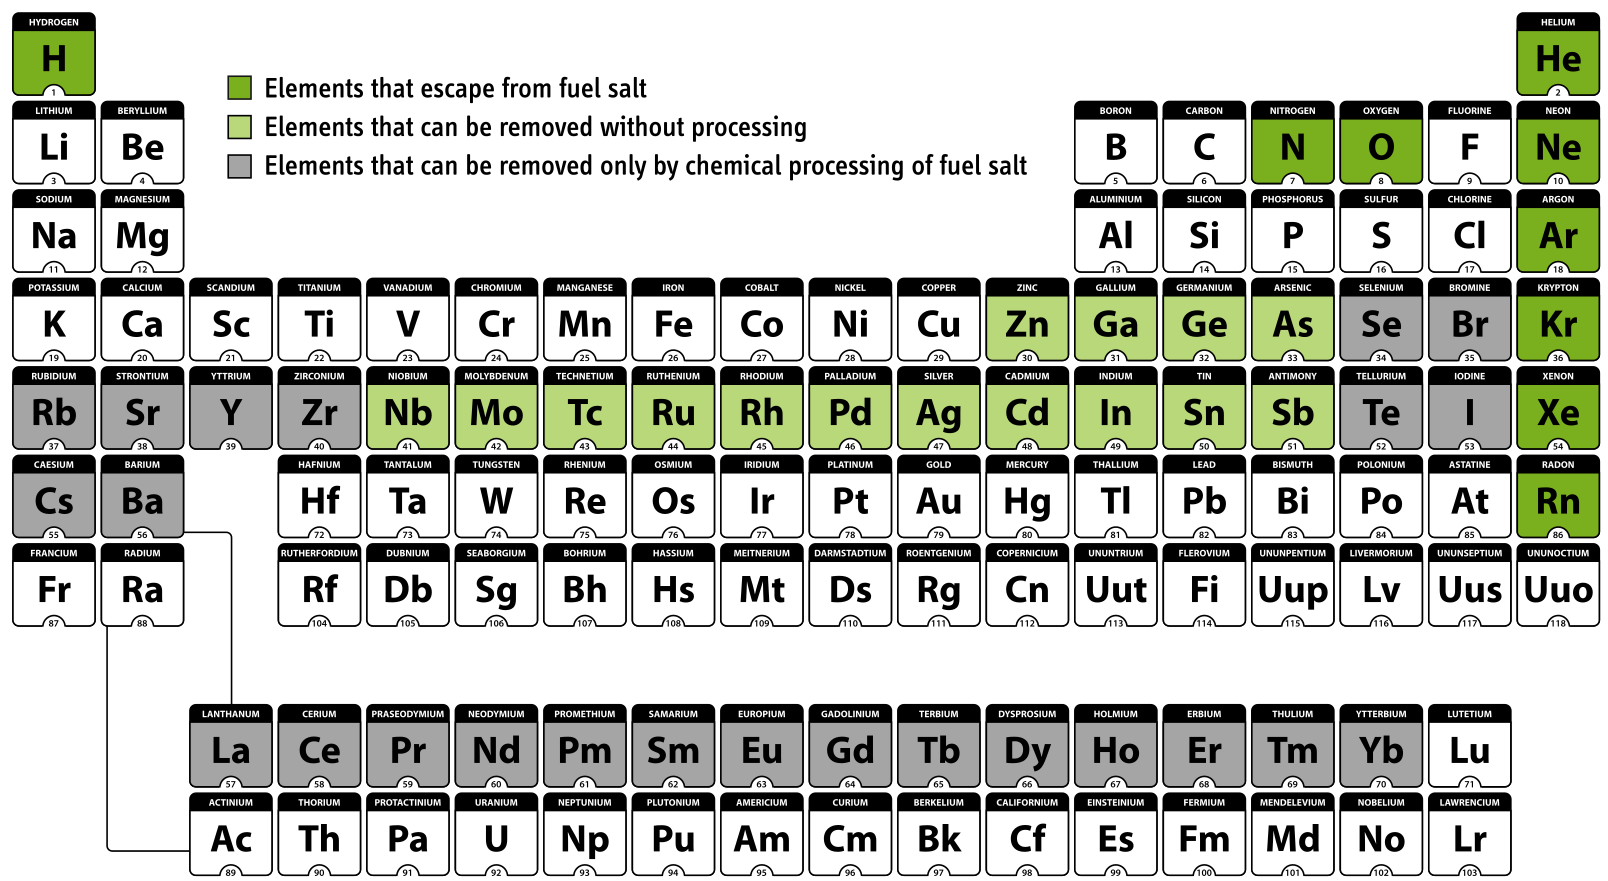
\includegraphics[width=0.9\textwidth]{periodic_map.png}
  \caption{Processing options for \gls{MSR} fuels (figure reproduced from 
  Ahmed \emph{et al.} \cite{ahmad_neutronics_2015}).}
  \label{fig:periodic_tab}
\end{figure}

Most liquid-fueled nuclear reactor concepts adopt nonintermittent separations 
and feeds: the core material is circulated to or from the core at all times 
(continuously) or specific intervals (batch-wise). In contrast, in a 
solid-fueled reactor, fission products and actinides remain within the initial 
fuel material during and after the operation until reprocessing. The ability 
to perform online fuel salt reprocessing improves the potential neutronics 
performance of liquid-fueled reactors. First, liquid-fueled reactors can 
operate with a relatively small excess reactivity because fissile material is 
continuously being added to the core. Second, continuously 
removing fission products, including strong absorbers (poisons) should 
significantly improve fuel utilization and decrease parasitic neutron 
absorption. Finally, for a breeder\footnote{\gls{CR} 
$\equiv$ fissile generated/fissile consumed: if CR $<$ 1, the reactor is a 
``converter''; CR $\equiv$ 1, an ``isobreeder''; CR $>$ 1, a 
``breeder.''} excess of fissile material might be continuously extracted  
from the core and used to start up new reactors. Nevertheless, the removal of 
each element from the liquid fuel salt presents a unique challenge in terms of 
chemical separation, storage, and disposal of the separated materials.

Continuous fuel salt reprocessing prevents the usage of most contemporary 
nuclear reactor fuel burnup software. To handle the material flows and 
potential online removal and feed of liquid-fueled systems, early \gls{MSR} 
simulation methods at \gls{ORNL}, which integrated neutronic and fuel cycle 
codes (i.e., Reactor Optimum Design (ROD) \cite{bauman_rod_1971}) into 
operational plant tools (i.e., Multiregion Processing Plant (MRPP) 
\cite{kee_mrpp_1976}) for \gls{MSR} fuel reprocessing system design. A summary 
of recent efforts is listed in table~\ref{tab:msr_codes}.
\begin{table}[t]
\fontsize{9}{11}\selectfont
\caption{Tools and methods for liquid-fueled \glspl{MSR} fuel salt depletion 
analysis.}
\begin{tabularx}{\textwidth}{X X X X X} 
\hline 
&Nuttin \emph{et al.}, 2005 \cite{nuttin_potential_2005}& Aufiero \emph{et al.}, 
2013 \cite{aufiero_extended_2013} & Betzler \emph{et al.}, 2018 
\cite{betzler_fuel_2018}&Proposed work \\ [12pt]
\hline
Neutron transport software & \gls{MCNP} & Serpent 2 & SCALE6.2 & Serpent 2 \\ 
[12pt]
Neutron transport method & \multicolumn{2}{c}{Monte Carlo continuous energy} & 
Deterministic discrete ordinates & Monte Carlo continuous energy \\ [12pt]
Burnup software & REM & Serpent 2 & ORIGEN-S & Serpent 2 \\ 
[12pt]
Geometry model & unit cell & full-core 3D & unit cell & full-core 3D\\ [12pt]
\gls{FP} removal/feed  & continuous &continuous & batch-wise & batch-wise\\ 
[12pt]
Separation efficiency &\multicolumn{3}{c}{fixed, must be defined by user 
before simulation} & variable of many parameters \\ [12pt]
Fuel reprocessing plant & \multicolumn{3}{c}{single component, ``black'' box 
model} & realistic multi-component model \\ [12pt]
Reactivity control & \multicolumn{2}{c}{continuous adjustment of fissile 
material injection} & batch injection of fissile material & periodical 
adjustment of geometry and fissile material injection\\
\hline
\end{tabularx}
  \label{tab:msr_codes}
\end{table}

Two main online reprocessing simulation approaches are commonly used in the 
literature: continuous and batch-wise. In the batch-wise approach, the burnup 
simulation stops at a given time and restarts with a new liquid fuel 
composition (after removal of discarded materials and addition of 
fissile/fertile materials). 

Accounting for continuous removal or addition of material presents a greater 
challenge since it requires adding a term to the Bateman equations. In 
SCALE/TRITON, ORIGEN \cite{gauld_isotopic_2011} solves a set of the Bateman 
equations using one-group averaged fluxes and cross sections obtained from a 
transport calculation. The Bateman equations describe the rate of change of 
each isotope, $i$, due to neutron induced reactions and decay processes
\cite{tsoulfanidis_nuclear_2013}:
\begin{align} \label{eq:bateman}
\frac{dN_i}{dt} &= \sum_{m=1}^{M}l_{im}\lambda_mN_m + 
\phi\sum_{m=1}^{M}f_{im}\sigma_mN_m - (\lambda_i + \phi\sigma_i + r_i - 
f_i)N_i + F_i\Big|{i\in [1,M]}\\
& \qquad\qquad (1) \qquad\qquad\qquad (2) \qquad\qquad(3) \quad (4)  \quad 
(5) \quad (6)
\nonumber
\intertext{where}
N_i &= \mbox{atom density of nuclide i} \nonumber \\
M &= \mbox{number of nuclides} \nonumber \\
l_{im} &= \mbox{fraction of decays of nuclide m that result in formation of 
nuclide i}\nonumber \\
\lambda_i &= \mbox{radioactive decay constant of nuclide i} \nonumber \\
\phi &= \mbox{neutron flux, averaged over position and energy} \nonumber \\
f_{im} &= \mbox{fraction of neutron absorption by nuclide m leading to the 
formation of nuclide i} \nonumber \\
\sigma_m &= \mbox{average neutron absorption cross section of nuclide m} 
\nonumber \\
r_i &= \mbox{continuous removal rate of nuclide i from the system} \nonumber \\
f_i &= \mbox{continuous feed rate of nuclide i} \nonumber \\
F_i &= \mbox{production rate of nuclide i directly from fission}\nonumber
\end{align}
The four terms on the right-hand side of the equation represent:
\begin{enumerate}[label=(\arabic*)]
	\item production of species $i$ as a result of the decay of all the 
	nuclides present;
	\item production of species $i$ as a result of neutron capture by all 
	nuclides present;
	\item loss of nuclide $i$ through its own decay;
	\item loss of nuclide $i$ as a result of neutron capture;
	\item loss of nuclide $i$ through continuous removal from the system;
	\item gain of nuclide $i$ as a result of continuous feed to the 
	system.
\end{enumerate} 

Recently, Nuttin \emph{et al.} developed in-house depletion code REM which 
directly couples with \gls{MCNP} \cite{noauthor_mcnp_2004} to simulate fuel 
salt material evolution in a simplified \gls{MSBR}-like reactor. That work 
directly integrated the Bateman differential equations using neutron flux from 
the \gls{MCNP}, tracking all the isotopes available in the data library, and 
control reactivity to maintain reactor critical \cite{nuttin_potential_2005}.

In a similar vein, Aufiero \emph{et al.} extended Serpent 2 for continuous 
reprocessing simulations by explicitly introducing ``reprocessing'' time 
constants into the system of Bateman equations and adding effective decay and 
transmutation terms for each nuclide \cite{aufiero_extended_2013}. The 
developed extension directly accounts for the effects of online fuel 
reprocessing on depletion calculations and features a reactivity control 
algorithm. The extended version of Serpent 2 was assessed against a dedicated 
version of the deterministic ERANOS-based EQL3D procedure in 
\cite{fiorina_investigation_2013} and applied to analyze the \gls{MSFR} fuel 
salt isotopic evolution.

\gls{ORNL} researchers have developed ChemTriton, a Python script for
SCALE/TRITON which uses the batch-wise approach to simulate a continuous 
reprocessing and refill for either single or multiple fluid designs. 
ChemTriton models salt treatment, separations, discharge, and refill using a 
unit-cell MSR SCALE/TRITON depletion simulation over small time steps to 
simulate continuous reprocessing and deplete the fuel salt 
\cite{powers_new_2013, betzler_fuel_2018}.

Most of the existing tools represented fuel salt reprocessing plant as an 
invariable ``black box'' model which removes target elements all at once with 
a fixed efficiency, determined by the user before starting the depletion 
simulation. Typically, such a ``black box'' model is characterized by vector of  
removing elements and their extraction efficiencies:
\begin{equation}
\begin{bmatrix}
N^{in}_{0} \\ \vdots \\ N^{in}_{e} \\ \vdots \\ N^{in}_{E} \\
\end{bmatrix} 
\times
\begin{bmatrix}
\epsilon_{0} \\ \vdots \\ \epsilon_{e} \\ \vdots \\ \epsilon_{E} \\
\end{bmatrix} =
\begin{bmatrix}
N^{out}_{0}\\ \vdots \\ N^{out}_{e} \\ \vdots \\N^{out}_{E}  \\
\end{bmatrix}
\end{equation}
where $N^{in/out}$ is the number density of atoms and $\epsilon$ is the 
extraction efficiency for all elements $e$ in $(0, E)$. The main issues 
related with static ``black box'' model assumptions in the literature include: 
\paragraph{Time-independent separation efficiency vector.} Realistically, 
	long-term reactor operation will require a time-dependent extraction 
	efficiency vector.
\paragraph{The separation efficiency is independent of the reactor operational 
	parameters.} In reality the extraction efficiency depends on temperature, 
	power level, current fuel salt isotopic composition, and material mass 
	flow rate.
\paragraph{All reprocessing plant components are treated as a single ``black 
box'' component.} However, the fuel salt in a reprocessing plant undergoes 
many separate components (e.g., helium bubbling, nickel mesh filter, etc.) 
which target specific elements. Some of these components can be connected in 
series, parallel, or series-parallel. The ``black box'' model (only single 
process) requires massive pre-simulation analytic work from the user to 
calculate lumped separation efficiency vector before a simulation is run and 
cannot be adjusted during the simulation. Additionally, treating the 
processing system as a single ``black box'' may lose dynamics. Finally, the 
waste stream from each component cannot be tracked separately, which is 
necessary for fuel reprocessing system optimization.

Some of the tools listed in table~\ref{tab:msr_codes} used major 
approximations that may lead to inaccurate fuel evolution predictions, and 
others are not available for external users. This work proposes an open-source 
simulation package, SaltProc, which expands the capability of the 
continuous-energy Monte Carlo Burnup calculation code, Serpent 2, for 
simulation liquid-fueled \gls{MSR} operation.

\subsection{Operational and safety parameters evolution} 
\label{sec:saf-par-literature}
In contrast with conventional solid-fueled reactors in which in-core fuel 
residence time is 4-5 years\footnote{For the most common 
18-month cycle, during refueling personnel removing 1/3 of the fuel 
assemblies, re-arranging other assemblies, and loading fresh fuel into the 
core. Thus, each fuel assembly is kept in the core at most $3\times 18=54$ 
months.}, the initial fuel salt batch stays in the \gls{MSR} reactor primary 
loop during the whole lifetime. Therefore, the fuel salt accumulates 
\glspl{FP} not captured by fuel reprocessing system as well as transuranic 
elements\footnote{The chemical elements with atomic numbers greater than 
uranium (92).}. Continuous fuel salt composition evolution has a 
significant influence on the neutron energy spectrum and, consequently, 
affects the reactor behavior, necessitating additional safety analysis.

Nuttin \emph{et al.} studied evolution of a key safety parameter, the 
temperature 
reactivity feedback coefficient, estimating it for the \gls{MSBR} at start-up 
and at equilibrium. The temperature coefficient of reactivity quantifies 
reactivity changes due to temperature increase in the core and was calculated 
in that 
work as:
\begin{align}\label{eq:feedback}
& \qquad\qquad\qquad \alpha = \frac{k_{1200} - k_{900}}{\delta T} 
\intertext{where}
k_{900}, k_{1200}  &= \mbox{the multiplication coefficients at 900K and 
1200K, respectively} 
\nonumber \\
\delta T &= 1200K-900K.\nonumber
\end{align}
That work showed that the \gls{FTC} at start-up and at equilibrium is $-1.5$ 
and $-1.0pcm/K$, respectively. Percent mille ($pcm$) is the unit of reactivity 
equal to $10^{-5}$ of $k_{eff}$.
Nuttin \emph{et al.} also reported a positive and time-invariant 
total temperature coefficient ($+0.8pcm/K$) \cite{nuttin_potential_2005}. 
Recently, Park and colleagues expanded that approach to a full-core 
high-fidelity \gls{MSBR} model and estimated safety parameters evolution over 
20 years of operation \cite{park_whole_2015}. These calculations showed 
relatively large negative total temperature coefficient during 20 years of the 
reactor operation; the coefficient magnitude weakens from $-3.21$ to 
$-1.41pcm/K$ at start-up and at equilibrium composition, respectively. 
Additionally, that work reported control rod worth deterioration from 
$2099pcm$ to $1970pcm$ due to neutron spectrum hardening during reactor 
operation. 

More recently, Betzler \emph{et al.} \cite{betzler_assessment_2017} reported 
key safety parameters evolution for the \gls{TAP} \gls{MSR}: the fuel 
reactivity coefficient at \gls{BOL} and 15 years from \gls{BOL} is negative 
and decreasing slowly over the reactor lifetime; the moderator reactivity 
coefficient is small and positive at \gls{BOL} and became negative after 15 
years of operation. Overall, thermal feedback seems to be stronger in the 
\gls{TAP} reactor and deteriorates insignificantly during the reactor 
operation. Notably, the authors ignored material density change with 
temperature to simplify temperature coefficients calculation; thus, only  
Doppler broadening was taken into account. Finally, the researchers reported 
the total worth of all control rods in the \gls{TAP} core at start-up only. 

The evolution of control rod worth in the \gls{TAP} has not been reported in 
the literature before. The proposed work will illuminate the evolution of majo 
safety parameters (fuel, moderator and total temperature coefficient, void 
reactivity coefficient, control rod worth) for the \gls{TAP} \gls{MSR} at 
various moments during the reactor operation. Additionally, the impact of 
neutron poison accumulation (e.g., $^{135}$Xe) in the fuel salt during 
short-term transients (i.e., load following) on safety characteristics will be 
investigated.

\section{Background Summary}
State-of-the-Art software packages for depletion analysis and evolution of 
safety parameters in liquid-fueled \gls{MSR} are reviewed in this Chapter. 
Based on this summary, I have identified a few possible directions for 
the improvement of \gls{MSR} tools:
\paragraph{Reproducibility/Availability.}
Serpent is the only contemporary nuclear 
contemporary nuclear 
reactor physics software which can perform depletion calculations with taking 
into account online fuel salt reprocessing regime. However, this built-in 
online reprocessing routine is undocumented  and the discussion forum for 
Serpent users is the only useful source of information at the moment. 
Other mentioned tools are under the closed-source license or available for 
internal users only. These issues can be a barrier to reuse of research 
software and to reproduce scientific results. Thus, a new, open-source, 
reproducible tool for fuel processing simulation would assist in the 
production of reproducible research in the area of liquid-fueled reactor 
modeling.
\paragraph{Realistic fuel reprocessing system model.} 
Major approximations in fuel reprocessing parameters deteriorate fuel salt 
composition predictions since the evolution of safety parameter accuracy is 
strongly dependent on fuel salt composition. A realistic fuel reprocessing 
system model will allow reprocessing component parameter optimization,  
increase fidelity of fuel and waste stream composition calculations, and 
advance reprocessing system design.
\paragraph{Variable extraction efficiency.} Most of the research efforts in 
the literature assumed ideal 100\% extraction efficiency of all removed 
elements, which stayed 
constant during the whole reactor lifetime. But realistically the efficiency 
is time-dependent and changes with respect to operational parameters: 
temperature, power level, salt composition, etc. Thus, the ability to set up 
dynamic separation efficiency must be added in \gls{MSR} simulation tools to 
advance depletion calculations.
\paragraph{Reactivity control.} Reconfigurable moderator configuration in the 
\gls{TAP} core presents a challenge because of the core geometry changes with 
respect to time. The reactivity control module which adjusts the core geometry 
to maintain criticality would be a great capability for simulating a new, more 
advanced \gls{MSR} concepts and short-term transients.
\paragraph{Safety characteristics evolution during reactor operation.} The 
\gls{MSR} fuel salt  accumulates \gls{FP} and transuranic elements which 
significantly shift neutron energy spectrum. Neutron energy hardening might 
worsen the core safety during operation. The impact of the fuel salt evolution 
on the \gls{MSR} safety parameters must be carefully investigated and reported.

The proposed work will hopefully overcome these issues and demonstrate the 
tool capabilities for promising \gls{TAP} \gls{MSR} concept.
	% for INTRODUCTION in "intro.tex"
\chapter[Online reprocessing modeling and safety analysis]{Online reprocessing 
modeling and safety analysis}
\section{Fuel salt reprocessing plant overview}
Removing specific chemical elements from a molten salt is a complicated 
task that requires intelligent design (e.g., chemical separations equipment 
design, fuel salt flows to equipment) and has a considerable economic cost. 
This section contains a brief overview of fuel reprocessing system of generic 
\gls{MSR}.

\subsection{Gas separation system}
Gaseous fission products (e.g. Kr, Xe) must be removed from the fuel salt 
to avoid reactor poisoning especially during startup and power maneuvering. 
This is particularly true for $^{135}$Xe, with its very large neutron capture 
cross section (2.65$\times$10$^6$ b). The $^{135}$Xe ultimate yield from 
fission is about 6.4\%, most of this is from fission-produced $^{135}$I and 
$^{135}$Te decay (table~\ref{tab:xe_gain}). Noble gas (tritium, xenon, and 
krypton) can be removed from the fuel salt as follows: (1) a bubble generator 
injects helium bubbles in the salt stream; (2) noble gas mitigate promptly 
to the helium bubbles because of their exceptional insolubility in the salt; 
(3) a gas separator removes the fission-product-rich bubbles from
the salt 
and discharged it to the off-gas system. Diagram~\ref{fig:xe_diagram} shows 
the main ways of xenon production, accumulation, and removal in the typical 
\gls{MSR}.
%%%%%%%%%%%%%%%%%%%%%%%%%%%%%%%%%%%%%%%%%%%%%%%%%%%%%%%%%%%%%
\begin{table}[ht!]
	\caption{$^{135}$Xe production sources and principal rate constants 
		involved
		(reproduced from Kedl \emph{et al.} \cite{kedl_development_1967}).}
	\centering
	\begin{tabularx}{\textwidth}{b  b}
		\hline \textbf{$^{135}$Xe gain mechanism} & \textbf{Principal rate 
			parameters involved}  	\\ \hline 
		Direct from fission & $\nu \Sigma_f \gamma_{^{135}Xe}\phi$ (for 
		$^{235}$U fission) \\ 
		yield $\gamma_{^{135}Xe}=0.003$ & \\ \hline
		$^{135}$I decay       & $\nu \Sigma_f \gamma_{^{135}I}\phi$ (for 
		$^{235}$U fission) \\
		yield $\gamma_{^{135}Xe}=0.036$, it decays to $^{135}$Xe with 
		$\tau_{1/2}=6.68$ h & 			                    \\		\hline
		$^{135}$Te decay      & 
		$\nu \Sigma_f \gamma_{^{135}Te}\phi$ (for $^{235}$U fission) \\
		yield $\gamma_{^{135}Xe}=0.025$, 
		it quickly decays to $^{135}$I with $\tau_{1/2}=19$ s 
		& 			                    \\	\hline 
	\end{tabularx}
	\label{tab:xe_gain}
\end{table}
%%%%%%%%%%%%%%%%%%%%%%%%%%%%%%%%%%%%%%%%%%%%%%%%%%%%%%%%%%%%%%%%%%%

Figure~\ref{fig:gas_removal_system} shows principal design of the \gls{MSBR} 
gas separation system. Helium bubbles of specific size are introduced in a 
salt stream via the primary pump bowl; these bubbles absorbed noble gas 
before being separated from the salt by a gas separator. The \gls{ORNL} proved 
that the \gls{MSBR} gas separation system can remove up to 99.5\% of 
$^{135}$Xe. Such a exceptional separation efficiency can be achieved by 
injecting helium bubbles of $d=0.508$ mm, and redirecting 10\% of the fuel 
salt flow from the pump discharge through a bubble separator to remove the 
xenon bubbles and then back into the pump suction. Robertson \emph{et al.} 
reported that helium bubble size was approximately 25\% of the 
throat width (blue circle on figure~\ref{fig:bubble_separator}) and was 
independent of the gas flow rate \cite{robertson_conceptual_1971}. 
Consequently, it is possible to regulate helium bubble size by changing throat 
width in the bubble generator.
\begin{figure}[htp!] % replace 't' with 'b' to 
	\centering
	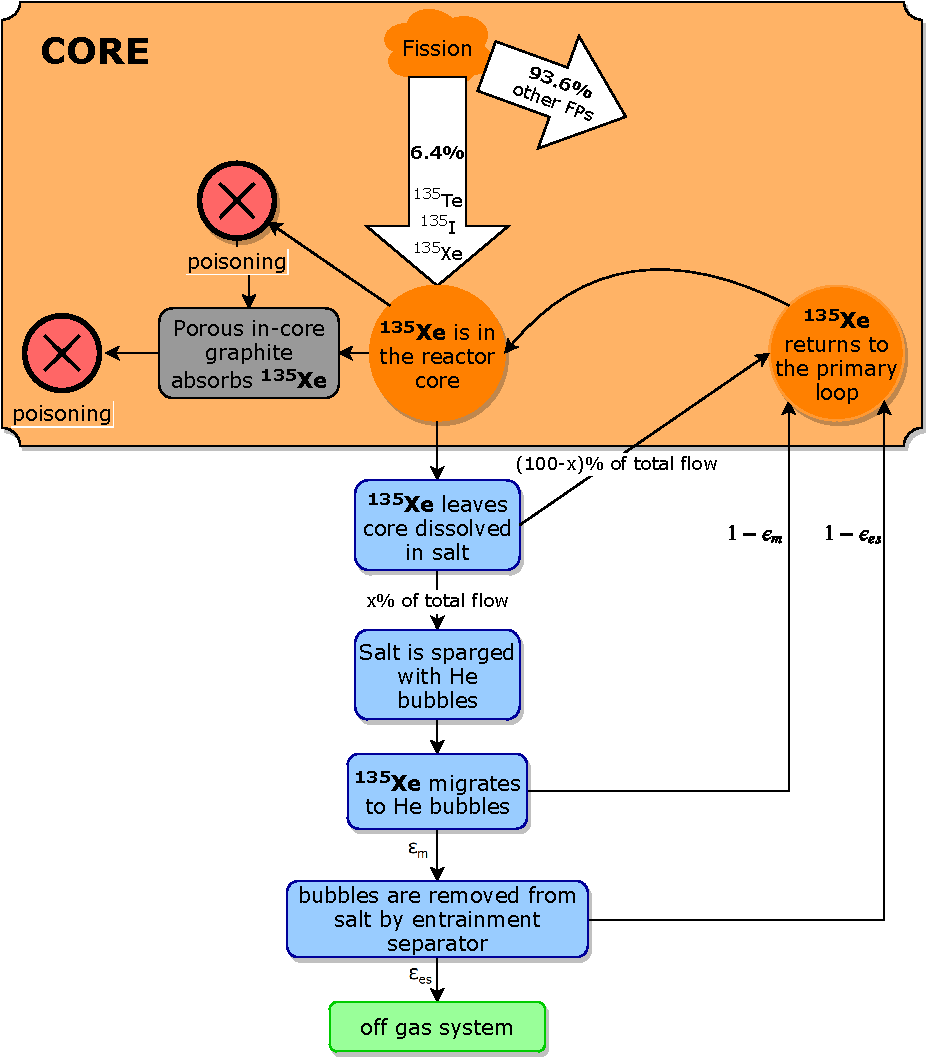
\includegraphics[width=\textwidth]{xe_diagram.pdf}
	\caption{Schematic $^{135}$Xe circulation diagram in a generic \gls{MSR}. 
	The $\epsilon_m$ is the migration efficiency of $^{135}$Xe to the helium 
	bubbles and $\epsilon_{es}$ is the gas separation efficiency in the 
	entrainment separator. The orange color represents the active core region, 
	the blue color represents the gas separation system, and the gray color is 
	moderator in the core,}
	\label{fig:xe_diagram}
\end{figure}
\begin{figure}[htp!] % replace 't' with 'b' to 
  \centering
  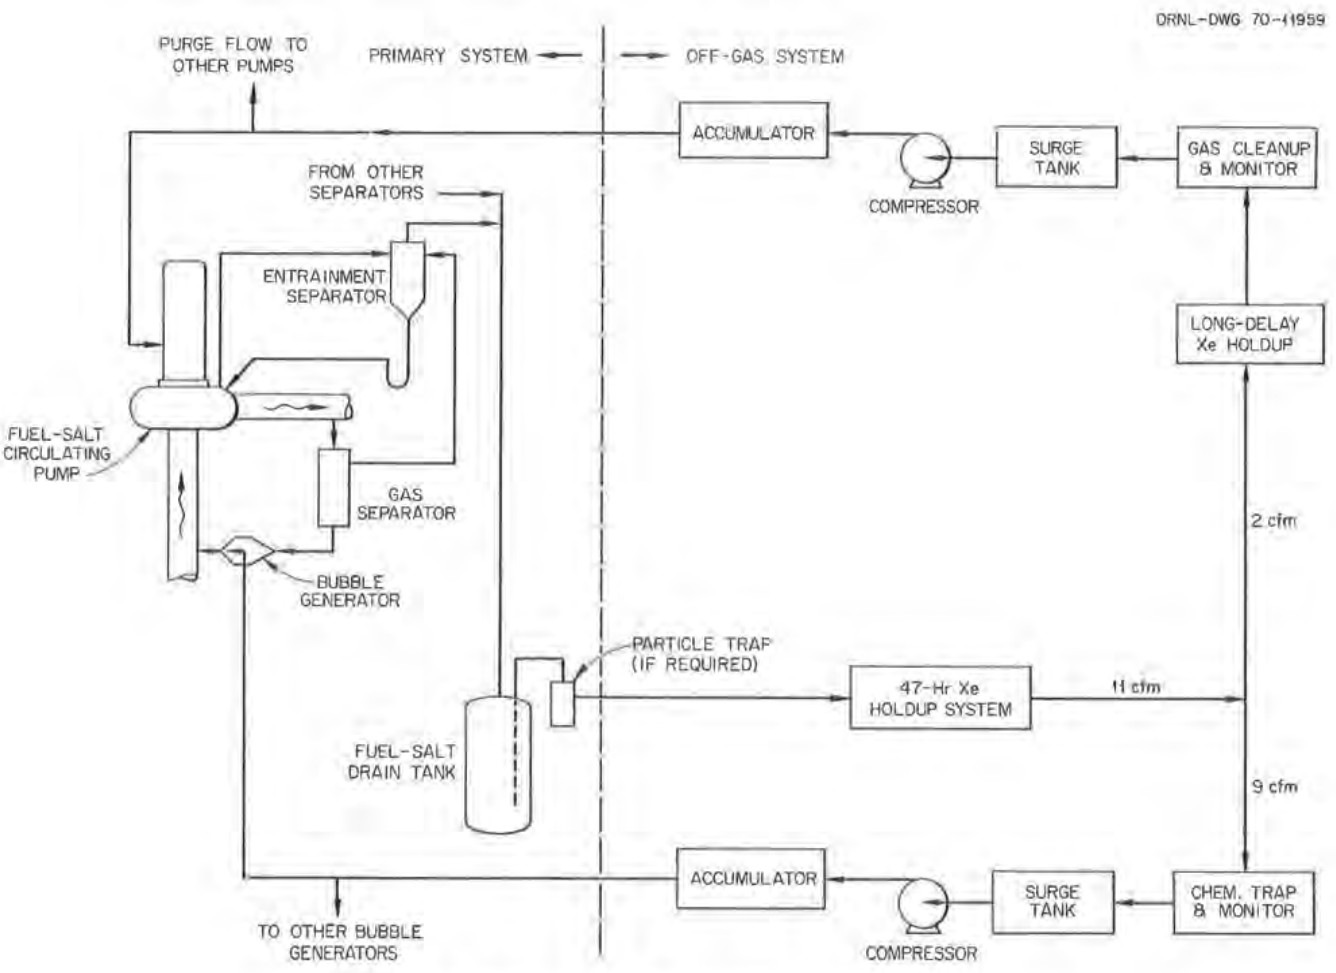
\includegraphics[width=\textwidth]{gas_separation.png}
  \caption{Schematic flow diagram of the \gls{MSBR} gas separation system 
  (figure reproduced from Robertson \emph{et al.} 
  \cite{robertson_conceptual_1971}).}
  \label{fig:gas_removal_system}
\end{figure}
\begin{figure}[t] % replace 't' with 'b' to 
  \centering
  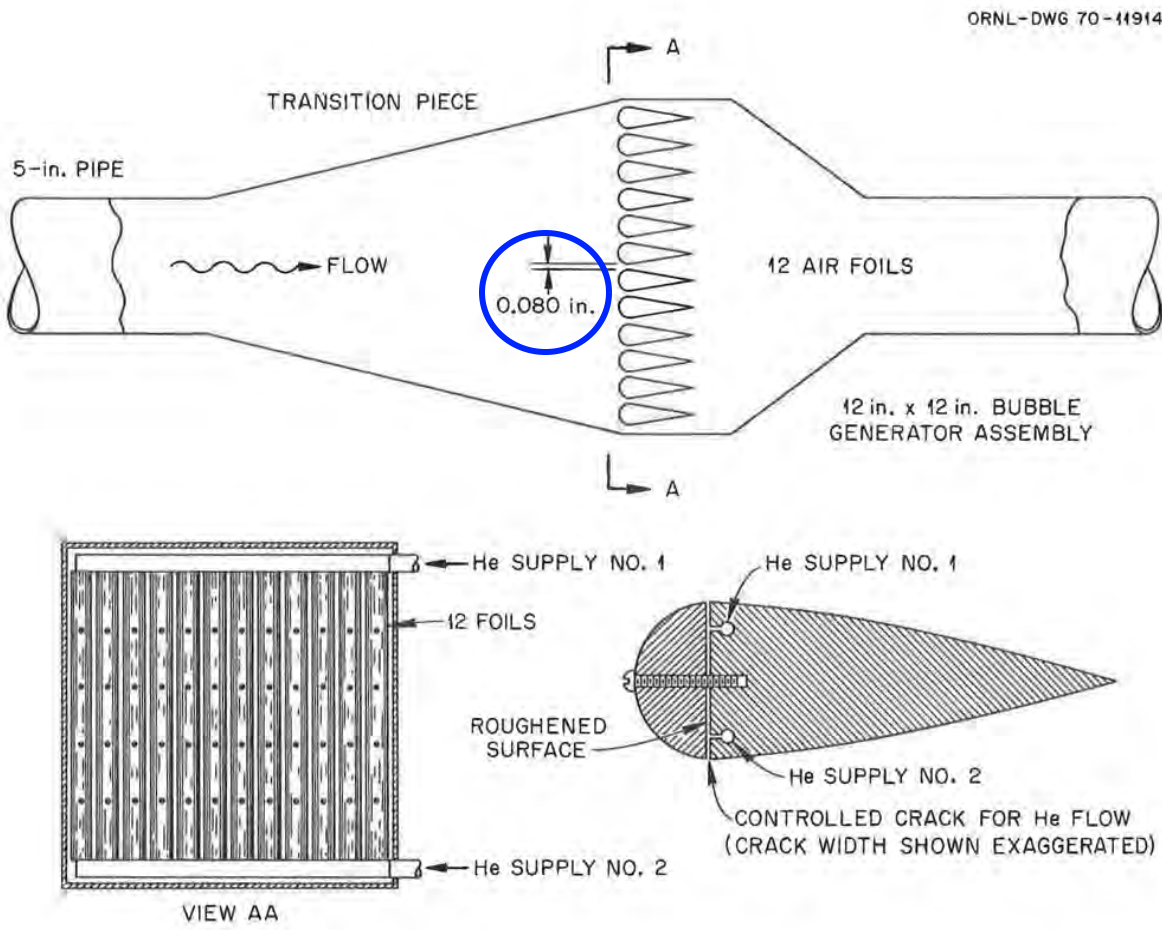
\includegraphics[width=0.8\textwidth]{msbr_bubble_generator.png}
  \caption{Preliminary concept of \gls{MSBR} bubble generator (figure 
  reproduced from Robertson \emph{et al.} \cite{robertson_conceptual_1971}). 
  The blue circle shows 
  throat width, which determines bubble size.}
  \label{fig:bubble_separator}
\end{figure}
\begin{table}[b]
	\caption{$^{135}$Xe loss terms and principal rate constants involved
		(reproduced from Kedl \emph{et al.} \cite{kedl_development_1967}).}
	\centering
	\begin{tabularx}{\textwidth}{b b}
		\hline \textbf{$^{135}$Xe loss mechanism}      & \textbf{Principal 
		rate 
			parameters involved}  	\\
		\hline Decay of dissolved $^{135}$Xe ($\tau_{1/2}=9.1$ h)  & Decay 
		constant	($\lambda$)		\\
		\hline $^{135}$Xe burnup              &  Neutron flux 
		($\Phi$)		 					\\
		dissolved xenon-135 burnup as it passes throught core  
		& 			            \\		\hline $^{135}$Xe transferred to 
		off-gas system via xenon stripper & Stripping efficiency 
		($\epsilon$)		\\
		\hline $^{135}$Xe transferred into circulating He bubbles; this xenon 
		will eventually be burnup, decay, or stripped via bubble separator & 
		Mass transfer coefficient ($h$), decay constant ($\lambda$), 
		neutron flux ($\phi$), bubble removing efficiency ($\epsilon$)		\\
		\hline 
	\end{tabularx}
	\label{tab:xe_loss}
\end{table}

To realistically model the gas separation system, a mathematical model 
describing noble gas extraction efficiency dynamics during reactor operation 
is required. Particularly, a model of xenon extraction efficiency as a 
function of a sparger design parameters is needed to accurately model 
$^{135}$Xe removal in a fuel salt depletion simulation. The gain and loss 
terms for $^{135}$Xe dissolved in the fuel salt are listed in 
Tables~\ref{tab:xe_gain} and \ref{tab:xe_loss}. The stripping efficiency for 
the xenon in the pump bowl has been measured during the \gls{MSRE} but the 
technical report ORNL-4069 by Kedl-Houtzeel only stated its range (from 50 to 
100\%) and mentioned that the results are not accurate 
\cite{kedl_development_1967}. $^{135}$Xe burnup and decay rates are well 
known. 

Previous research by \gls{ORNL} \cite{peebles_removal_1968} has reported xenon 
removal efficiency ($\epsilon_{Xe}$) in a gas separation system as a function 
of many parameters:
\begin{align}
& \qquad\qquad \epsilon_{Xe} = \frac{1-e^{-\beta}}{1+\alpha}
	\intertext{where}
 	\alpha &= \frac{RTQ_{salt}}{HQ_{He}} \\
 	\beta &= \frac{K_L a A_C L (1+\alpha)}{Q_{salt}} \\
 	R &= \mbox{universal gas constant} \nonumber \\
 	T &= \mbox{salt temperature} \nonumber \\
 	Q_{salt}&= \mbox{volumetric salt flow rate} \nonumber \\
 	Q_{He}&= \mbox{volumetric helium flow rate} \nonumber \\
 	H &= \mbox{Henry's law constant for solute gas} \nonumber \\
 	a &= \mbox{gas-liquid interfacial area} \nonumber \\
 	A_C &= \mbox{contactor cross section} \nonumber \\
 	L &= \mbox{contactor length} \nonumber \\
  	K_L &= \mbox{liquid phase mass transfer coefficient} \nonumber
\end{align}
Most of input parameters for that correlation are obvious and easy to obtain 
from the system component design. The mass transfer coefficient for 
transferring xenon into helium bubbles ($K_L$) can be estimated from 
experiment or CFD-model but published information is insufficient to inform an 
accurate mathematical model\footnote{Peebles \emph{et al.} reported the mass 
transfer coefficient for the \gls{MSBR} salt (LiF-BeF$_2$-ThF$_4$-UF$_4$) but 
at stationary flow conditions. While it is out of the scope of this work to 
accurately estimate mass transfer coefficient, this work seeks to provide tool 
which will allow user to specify any mathematical model for a separation 
efficiency.}.

This technique would be applicable to other noble gases (e.g. Kr) but the 
correlation coefficients would be different. To create a realistic 
mathematical model, an interfacial mass transfer coefficients for various 
volatile gases (particularly xenon) are needed. These coefficients can be 
obtained experimentally or using CFD simulations. Current effort at the 
University of Illinois at Urbana-Champaign namely, ``Enabling Load Following Capability in the Transatomic Power \gls{MSR}" \cite{huff_enabling_2018}, have a goal to determine the coefficients using CFD simulations and verify them in small experiments. As a result, the obtained mathematical model for a gas removal efficiency will be used to inform 
realistic physics-based fuel reprocessing model in the proposed SaltProc tool.

\subsection{Fuel salt chemical processing facility} \label{sec:chemical_processing}
Additionally to noble gas (e.g., Xe, Kr), the fuel salt reprocessing system  
must extract other \gls{FP}: noble/semi-noble metals and lanthanides. They  
generally have a relatively low capture cross section and thus absorb fewer 
neutrons than $^{135}$Xe, but their removal is crucial to guarantee normal  
operation. Some fraction of noble and semi-noble solid fission products are 
plate out onto a internal surfaces of the primary loop equipment. Lanthanides 
have relatively high solubility in the carrier salt and must be removed by 
chemical extraction. 

Protactinium presents another challenge for thorium-fueled 
\glspl{MSR}\footnote{The $^{232}$Th in the fuel salt absorbs thermal neutrons 
and produces $^{233}$Pa which then decays into the fissile $^{233}$U.} (e.g., 
\gls{MSBR}, \gls{MOSART}), since it has a large absorption
cross section in  
the thermal energy spectrum. Accordingly, $^{233}$Pa is continuously removed 
from the fuel salt into a protactinium
decay tank to allow $^{233}$Pa to decay 
to $^{233}$U without poisoning the reactor. This feature allows the 
thorium-fueled \gls{MSR} to avoid neutron losses
to protactinium, keeps 
fission products to a very low level, and increases the
efficiency of 
$^{233}$U breeding. 

Many authors reported liquid-liquid reductive extraction process as a best 
option for removing uranium and soluble fission products from 
molten fluoride salts \cite{briggs_molten-salt_1969, delpech_molten_2010, 
doligez_coupled_2014}. In that process the uranium or lanthanides can be 
selectively stripped from the salt into liquid bismuth due to different 
chemical potentials. Moreover, the \gls{MSRE} studies indicated that the 
extraction could be carried out rapidly and continuously  
\cite{whatley_engineering_1970-1}.

The principal scheme of the \gls{MSBR} reprocessing facility concept is shown 
in Figure~\ref{fig:material_flow}. The fuel salt is first temporarily stored 
for cooling and decay of the shortest lived fission products, then directed to 
the primary fluorinator. There most of the uranium is removed by fluorination 
to UF$_6$. After that, the salt is routed to an extraction column where the 
mixture containing metallic bismuth, lithium and thorium as reductants is 
contacted with the salt. The remaining uranium and protactinium are 
reductively extracted to a bismuth solution, leaving a salt that only contains 
fission products dissolved in carrier salt (base composition 
LiF-BeF$_2$-ThF$_4$). The salt then goes through a reduction column where 
UF$_6$ is reduced to UF$_4$ in the salt and preparing it for return to the 
reactor. BeF$_2$ and ThF$_4$ are also added and all residual bismuth is 
removed from the salt. After a final cleanup step and valence adjustment, the 
purified salt returns to the reactor \cite{carter_design_1972, 
sorensen_one-fluid_2006}.
\begin{figure}[htp!] % replace 't' with 'b' to 
  \centering
  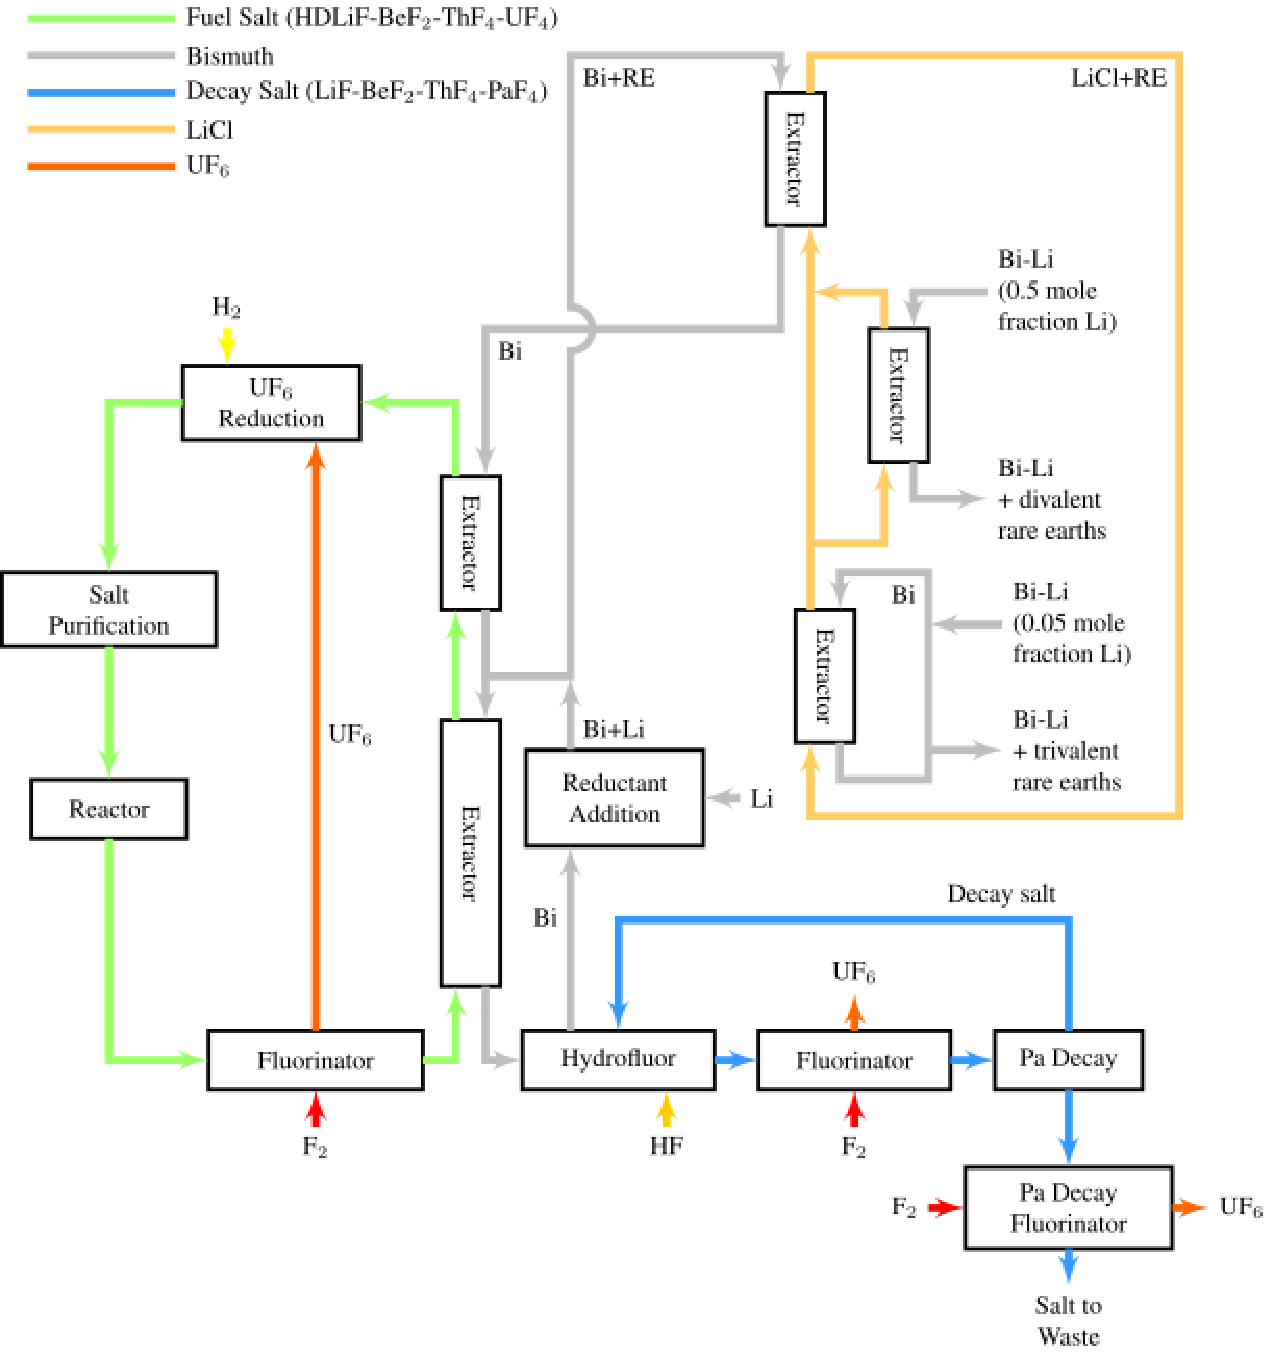
\includegraphics[width=0.9\textwidth]{flowsheet.pdf}
  \caption{Simplified block diagram of chemical processing scheme for 
  single-fluid \gls{MSBR} (reproduced from Sorensen 
  \cite{sorensen_one-fluid_2006}). \emph{RE} is a reducing agent.}
  \label{fig:material_flow}
\end{figure}

The bismuth accommodating some uranium and protactinium is routed to a 
hydrofluorination column where metallic solutes in the bismuth are 
oxidized into their fluoride forms in the presence of a decay 
salt\footnote{The decay salt contains UF$_4$, PaF$_4$, ThF$_4$ and fission 
products. Uranium produced after $^{233}$Pa decay is extracted and directed 
back into the reactor. Decay salt is the precursor for the waste salt as it 
was periodically discarded every 220 days.}. The decay salt, containing 
UF$_4$, PaF$_4$, and ThF$_4$, passed into a decay tank where $^{233}$Pa is 
decays to $^{233}$U. The uranium generated by protactinium decay is removed 
through fluorination to UF$_6$ and directed to the reduction column to refuel 
the purified fuel salt. A hydrofluorinator and a fluorinator can remove 
approximately 95\% of the uranium from the stream 
\cite{robertson_conceptual_1971}.

The fully processed salt, on its way back to the reactor, has uranium added 
from the protactinium decay tank at the rate required to maintain or adjust 
the uranium concentration in the reactor (and, consequently, control the 
reactivity). Adding fissile material is performed by sparging the salt with 
UF$_6$ and hydrogen to produce UF$_4$ in the salt and HF gas 
\cite{robertson_conceptual_1971}.

The fuel salt stream from the protactinium isolation system contains only 
traces of protactinium and uranium (because it was separated in the system) 
but contains practically all of the rare earths. A fraction of this salt 
stream is redirected to a reductive extraction process for removing rare 
earths.  The principal scheme of a rare earth removal system is shown in 
Figure~\ref{fig:rare-earth-removal}. A molten salt flow which contains 
rare-earth fluorides is fed to the center of an extraction column. The salt 
flows countercurrent to a liquid bismuth stream which contains thorium and 
lithium. In the upper part of the column, the rare earths are reduced and 
transferred to the downflowing liquid metal stream. Below the feed point, the 
rare earth concentration is increased in the salt and metal streams in order 
to produce a concentration high enough for disposal 
\cite{briggs_molten-salt_1969}.
\begin{figure}[htbp!]
	\centering
	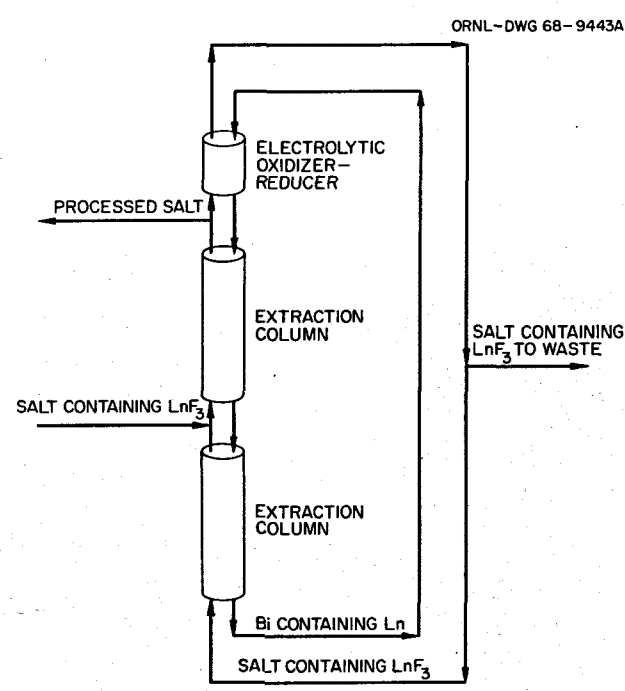
\includegraphics[width=0.45\textwidth]{rare-earths-removal-system.png}
	\caption{Rare earth removal from a fuel salt by reductive extraction 
	(figure 
		reproduced from Briggs \emph{et al.} \cite{briggs_molten-salt_1969}).}
	\label{fig:rare-earth-removal}
\end{figure}

Molten salt leaving the top of the column contains a dilute concentration of 
rare earths. A fraction of this flow is returned back to the reactor while the 
rest is sent to an electrolytic cell complex. The net effect of the complex is 
to push thorium and lithium into bismuth and to return extracted rare earths, 
entering the complex with bismuth from the bottom of the cascade, to the 
cascade as reflux, oxidizing them out of the metal and transferring them to 
the returning salt stream.

While it is out of the scope of proposed work to derive accurate 
chemistry-based mathematical formula for \glspl{FP} separation efficiency, 
this work seeks to provide a flexible tool that would be able to simulate 
chemical processes in a high-detailed level.

\section{SERPENT overview}
SERPENT is a continuous-energy Monte Carlo neutronics software capable of solving the neutron transport problem by tracking individual neutrons within the problem geometry and using stochastic method to determine chain of events for each neutron \cite{leppanen_serpent_2015}. SERPENT has been under active development at the VTT Technical Research Centre of Finland since 2004, where it was initially conceived as a tool to simplify group constant generation in a high-fidelity Monte Carlo environment. SERPENT is now widely used transport code  with a growing user base. Now SERPENT used by more than 500 registered individuals in 155 organizations located in 37 countries around the world. The burnup calculation capability in SERPENT is based on built-in calculation routines, without using any external solvers. A restart feature allows performing fuel shuffling or applying any modifications in the input by dividing the calculation into several parts, which is crucial for online reprocessing simulations.

The latest version, SERPENT 2, supports advanced geometries and has advanced burnup capabilities, including online refueling capabilities which are necessary for neutronic computations of pebble-bed reactors and liquid-fueled \glspl{MSR} \cite{aufiero_extended_2013}. Unfortunately, built-in online refueling features are still under active development and unavailable to ordinary users. Furthermore, recently multi-physics simulations using SERPENT 2 were demonstrated, including  calculations with thermal-hydraulics, \gls{CFD} and fuel performance codes \cite{leppanen_numerical_2015}. Two-way coupling to thermal-hydraulics, \gls{CFD}, and fuel performance codes operates on two levels: internal coupling to built-in solvers for fuel behavior and thermal-hydraulics and external coupling via a universal multi-physics interface. 

SERPENT 2 can be effectively run in parallel on computer clusters and multi-core workstations. Parallelization is handled by thread-based OpenMP, which enables all processsors to use shared memory space. Calculations can be divided into several nodes by distributed-memory \gls{MPI} parallelization. SERPENT 2  is an improvement upon SERPENT 1, and contains a complete redesign of memory management using hybrid OpenMP \cite{dagum_openmp_1998} + \gls{MPI} parallelization.  This hybrid parallelization is important in depletion calculations using computer clusters with multiple nodes, and allows to achieve significant speed-up in depletion calculations on computer clusters with more than 4'000 cores \cite{leppanen_serpent_2015}. 

All calculations herein were performed using SERPENT 2 version 2.1.30 on Blue Waters’ XE6 nodes. For cross section generation, the JEFF-3.1.2 nuclear data library was employed based on entirely open cross section data 
\cite{oecd/nea_data_bank_jeff-3.1.2_2014}. 

\section{Proposed simulation tool design and capabilities} \label{sec:tool_design}
The first version of the SaltProc Python tool for calculating \gls{MSR} fuel 
composition evolution taking into account an online reprocessing system 
was developed as a part of my M.Sc. thesis \cite{rykhlevskii_advanced_2018,
rykhlevskii_arfc/saltproc_2018}. The tool was designed to 
expand SERPENT 2 depletion capabilities for modeling liquid-fueled \gls{MSR} 
for online reprocessing. SaltProc uses HDF5 
\cite{the_hdf_group_hierarchical_1997} to store 
data and uses the PyNE Nuclear Engineering Toolkit \cite{scopatz_pyne_2012}
for SEPRENT output file parsing and nuclide naming. SaltProc is an 
open-source Python package that uses a batch-wise approach to simulate 
continuous feeds and removals in \glspl{MSR}. 

Capabilities of the developed tool, working with the Monte Carlo software 
SERPENT 2, were demonstrated using the full-core MSBR design for a 
simplified case with ideal removal efficiency (100\% of mass for target 
elements removed) \cite{rykhlevskii_modeling_2019}. Unfortunately, 
the code architecture and principal structure was not designed for 
flexible implementation of sophisticated online reprocessing systems 
including realistic physics/chemistry-based extraction efficiencies. 
Thus, complete refactoring of SaltProc using \gls{OOP} is needed to 
create a comprehensive generic tool to realistically model any \gls{MSR} 
reprocessing plant while taking into account variable extraction 
efficiencies, mass balance between the core and processing plant and 
reactivity control system.

\subsection{Proposed software architecture}
The SaltProc v2 Python toolkit will couple directly with SERPENT 2 input 
and output files, 
to allow the reprocessing system to couple to depletion calculation. 
Existing PyNE interfaces will be employed for SERPENT 2 output parsing as 
well as newly developed interfaces for input and output handling. 
Python 3 \gls{OOP} 
standard features will be used to create a flexible, user-friendly tool with 
great potential for further improvement and collaboration. 
Figure~\ref{fig:saltproc_class} shows the proposed SaltProc class structure 
 which includes 4 main classes:
\begin{enumerate}
	\item \textit{Depcode}. Contains attributes and methods for 
	reading the user's input file for the depletion software, initial 
	material (e.g., fuel and/or fertile salt) composition, principal 
	parameters for 
	burnup simulation (e.g., neutron population and number of cycles for Monte 
	Carlo), running the depletion code. The proposed work will only 
	support SERPENT 2 Monte Carlo (only 
	one instance of \textit{Depcode} will be instantiated) but in principle the 
	toolkit can support any depletion code (i.e. OpenMC 
	\cite{romano_openmc_2015}).
\begin{figure}[ht!] % replace 't' with 'b' to \centering
  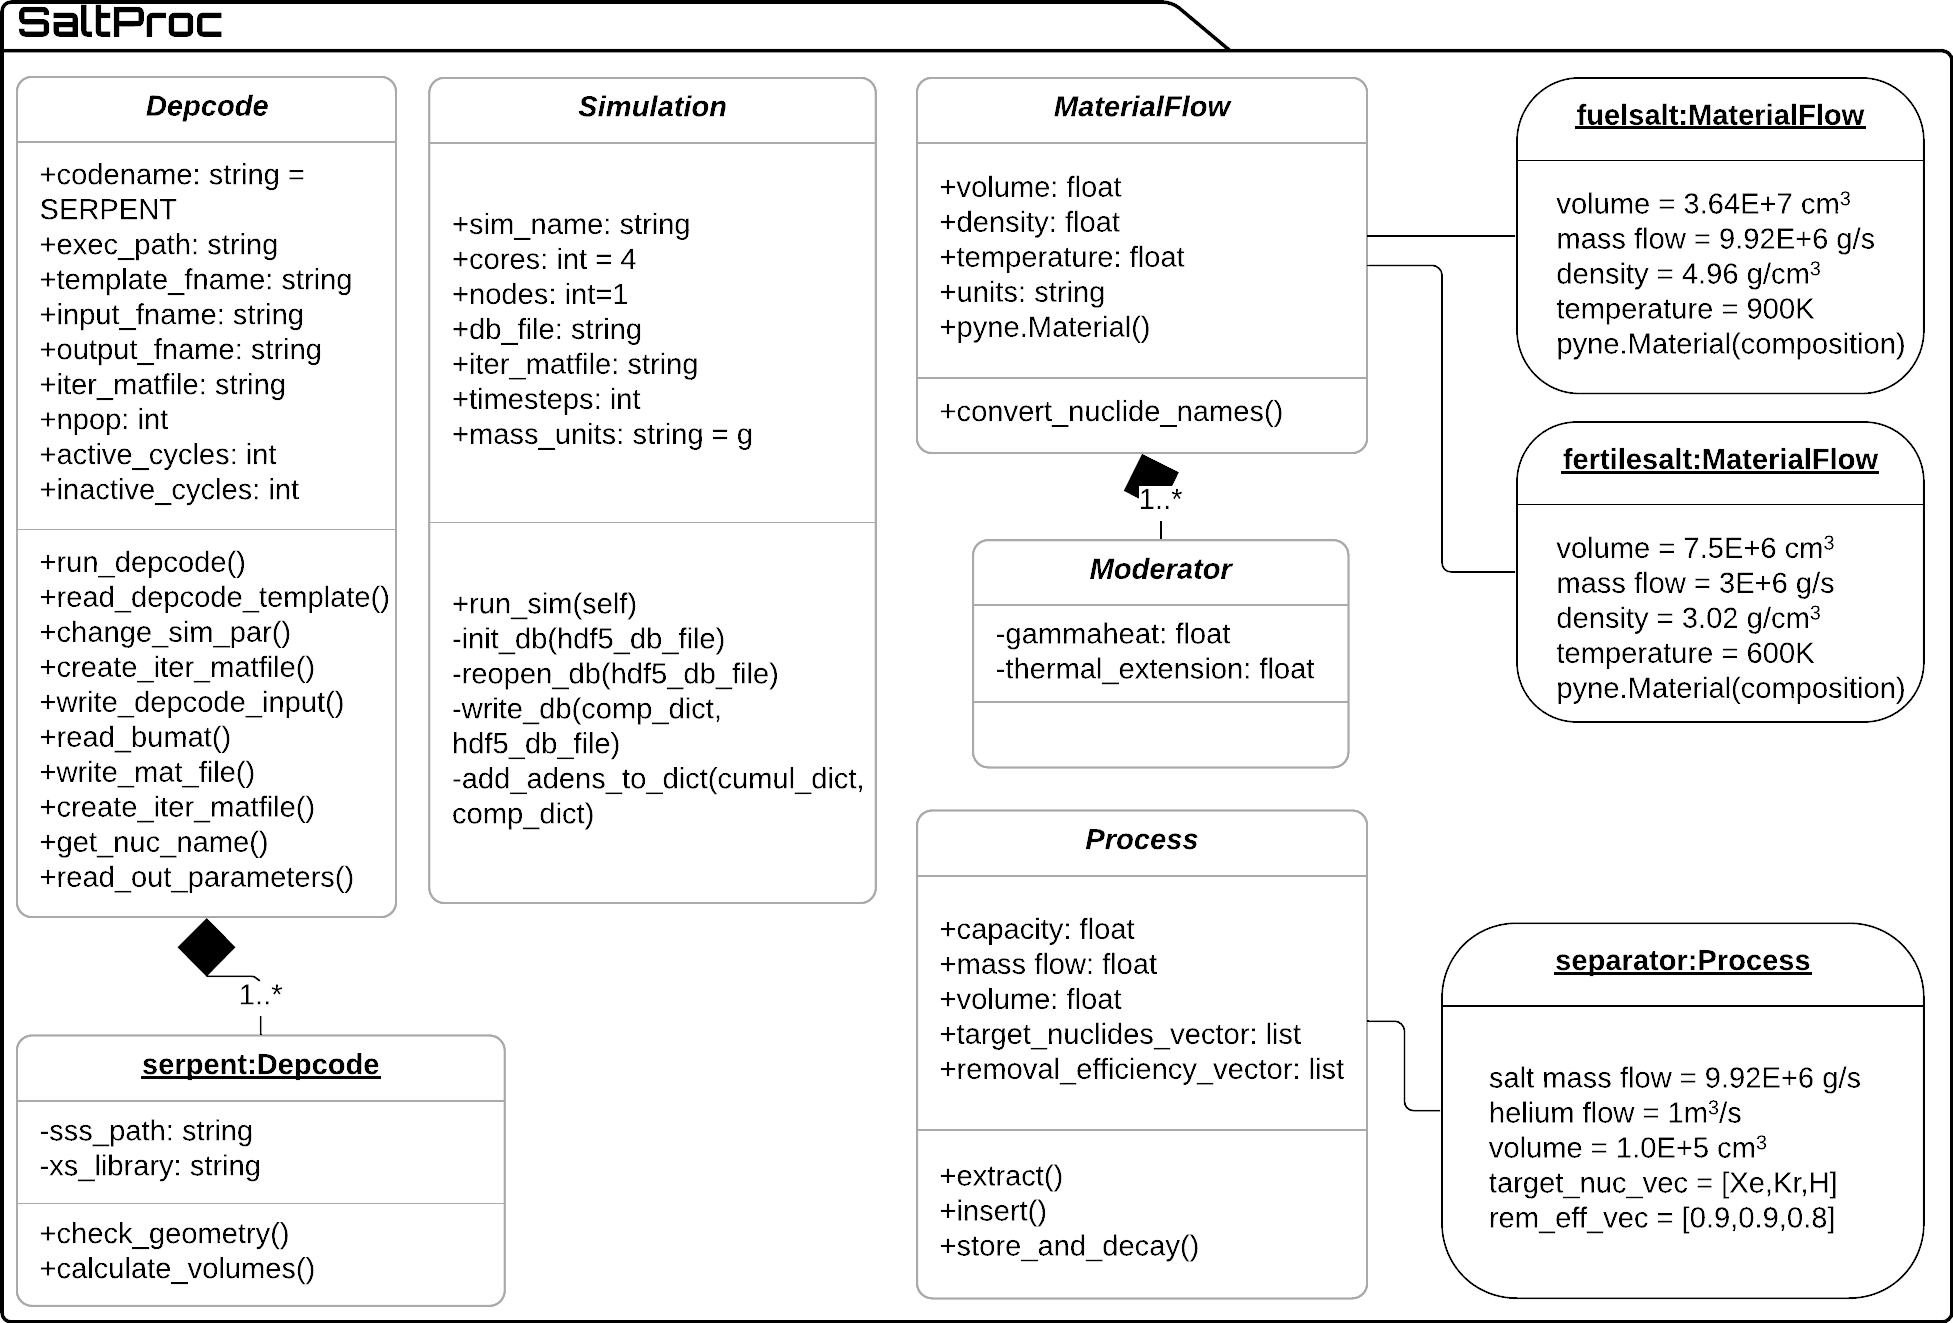
\includegraphics[width=\textwidth]{saltproc_class_diagram.png}
  \caption{Saltproc python package tentative class diagram with UML notation 
  and examples of object instances.}
  \label{fig:saltproc_class}
\end{figure}
	\item \textit{Simulation}. Runs SaltProc simulation step, 
	create, write HDF5 database, track time and convert 
	isotopic composition vector nuclide names from SERPENT to human 
	readable format. Also this class will allow simulation restart after 
	failure by restoring data from the HDF5 database and continue simulation 
	for additional depletion time.
	
	\item \textit{MaterialFlow}. Each \textit{MaterialFlow} object 
	will represent the material flowing between \textit{Process} objects. 
	The object of this class will contain an isotopic composition vector 
	(PyNE Material object 
	initialized	from SERPENT output file \textbf{dep.m}), mass flow rate, 
	temperature, density, volume, and void fraction. Existing PyNE Material 
	capabilities allows on to easily convert the units of isotopic 
	composition vector (e.g., from atomic density provided by SERPENT to 
	mass fraction or absolute mass in desired units), decay material 
	(i.e. model the \gls{MSBR} protactinium decay tank), calculate 
	decay heat, activity and dose. The main idea of the \textit{MaterialFlow} 
	object is to pass detailed information about the salt starting at the 
	\gls{MSR} vessel outlet throughout reprocessing facilities 
	(\textit{Processes}), which are modifying the \textit{MaterialFlow} 
	object before depleting the material in the next SERPENT burnup step.
		
	\item \textit{Process}. Each \textit{Process} object will represent a 
	realistic fuel processing step characterized by its throughput rate, 
	volumetric capacity, extraction efficiency for each target element (can be 
	function of many parameters), waste streams, and other parameters specific to 		the particular process. Refueling 
	\textit{Process} injects feed \textit{MaterialFlow} usually directly 
	into the reactor core (e.g., adding fissile material with specific mass flow 		rate to \textit{MaterialFlow} after performing all removals).
\end{enumerate}

The proposed class structure will provide outstanding flexibility in simulating 
various \gls{MSR} designs. A library of various \textit{MaterialFlow} (e.g., 
fuel salt flow, fertile salt flow, refueling salt flow) and \textit{Process} 
(e.g., helium sparging facility, gas separator, lanthanide removal component) 
objects will be created in this work to allow a user to quickly create a model 
of a desired reprocessing scheme. At runtime, the user will connect 
\textit{Process} objects in series or parallel with \textit{Flow} objects to 
form a comprehensive reprocessing system. The user will also be able to create 
a custom object with desired attributes and methods, and contribute back 
to the code package using Github (https://github.com/arfc/saltproc).	

\subsection{Tentative flowchart}
Figure~\ref{fig:saltproc_flow} illustrates the online reprocessing simulation 
algorithm coupling SaltProc and SERPENT 2. To perform a depletion step, 
SaltProc reads a user-defined SERPENT 2 template file. This file contains input 
 parameters such as geometry, material, isotopic composition, neutron 
population, criticality cycles, total heating power, and boundary conditions.  
After the depletion calculation, SaltProc reads the depleted fuel composition 
file and stores the depleted composition isotopic vector in an HDF5 database 
and \textit{MaterialFlow} object (\textit{CoreOut} in 
figure~\ref{fig:saltproc_flow}). This object contains an isotopic composition 
vector, total volume of material, mass flow rate, density and any other 
parameters specified by user. For the simplest reprocessing case, when all 
facilities are located in-line (100\% of total material flow goes through 
chain of separation components), the \textit{CoreOut} object is flowing 
sequentially between \textit{Processes} and each \textit{Process} is 
removing mass fraction of target elements with specified extraction 
efficiency. Afterward, the removed material mass will be compensated by 
fresh fuel salt to maintain the salt inventory in a primary loop. 
Finally, resulting isotopic composition from the \textit{ReprocOut} object will 
be stored in HDF5 database and dumped in a new composition file for the next 
SERPENT depletion run. 
\begin{figure}[ht!] % replace 't' with 'b' to \centering
  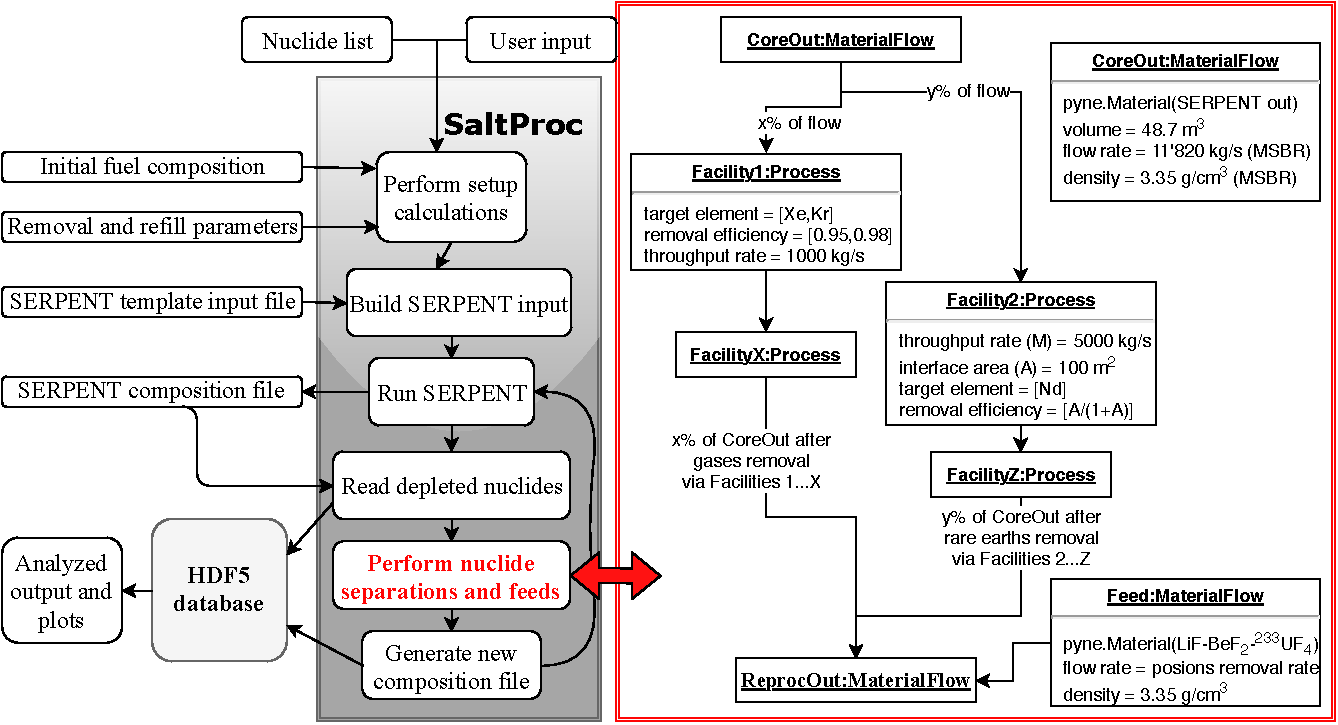
\includegraphics[width=1.05\textwidth]{saltproc_flowchart.pdf}
  \caption{Tentative generic flow chart for new Saltproc python package.}
  \label{fig:saltproc_flow}
\end{figure}

For a more general case with multiple concurrent extraction processes a separate 
\textit{MaterialFlow} object will be created for each branch with a user-defined 
mass flow rate (e.g. 90\% of total mass flow rate flows via left branch and 
10\% through right branch). Total volume and isotopic composition vector 
for each \textit{MaterialFlow} object will be calculated as a fraction of incoming 
\textit{CoreOut} flow. Then each \textit{MaterialFlow} object will be passed via 
a cascade of \textit{Processes} to separate selected chemical elements with 
specific efficiency. Finally, the left-hand-side branch \textit{MaterialFlow} object 
will be merged with the right-hand-side and similarly to previous case, fresh 
fuel salt feed will compensate the loss of mass in separation facilities and keep 
fuel salt mass in a primary loop constant.

The class diagram (Figure~\ref{fig:saltproc_class}) will allow simulating 
the operation of a complex, multi-zone, 
multi-fluid \gls{MSR} and is sufficiently general to represent myriad reactor 
systems. The refactored version of SaltProc will only store and edit the 
isotopic composition of the fuel stream, which makes it a flexible tool to 
model any geometry: an infinite medium, a unit cell, a multi-zone simplified 
assembly, or a full core. This flexibiliity allows the user to perform 
simulations of varying fidelity and computational intensity. SaltProc is an 
open-source tool (but a user needs SERPENT2 installed to use SaltProc), 
available on Github. It will leverage unit tests and continuous integration 
crucial for sustainable development. It will also have documentation
generated through Sphinx, a documentation generator, for ease of use. In summary, the 
development approach of SaltProc is focused on producing a generic, flexible and 
expandable tool to give the SERPENT 2 Monte Carlo code the ability to conduct 
advanced in-reactor fuel cycle analysis as well as simulate many 
online refueling and fuel reprocessing systems.

%\subsection{Reactivity control module}
%In addition, SaltProc will be able to define time-dependent material feed and 
%removal rates to investigate their impacts. These rates need not be 
%constant in SaltProc. They can be defined as piecewise functions or set to 
%respond to conditions in the core. For instance, SaltProc might increase the 
%fissile material feeding rate if the effective multiplication factor, 
%$k_{eff}$, falls below a specific limit (e.g., 1.002).
%These capabilities allow SaltProc to analyze fuel cycle of a generic 
%liquid-fueled \gls{MSR}.


\chapter[Code demonstration and validation]{Code demonstration and validation}

After refactoring, redesign, and implementation of the new capabilities 
mentioned in Chapter 3, SaltProc v2.0+ will be tested for the \gls{TAP} 
\gls{MSR}. I selected the \gls{TAP} concept because it is well analyzed in the 
literature; thus, cross-code verification with ChemTRITON/SCALE is possible 
\cite{betzler_assessment_2017}. The demonstration will be performed for two 
timescales:
\paragraph{Long-term.} The reactor lifetime-long (e.g., 40 years) depletion 
simulation will be performed with moderate time resolution (e.g., 30-day 
depletion step). The results obtained with SaltProc v2.0+ will be compared 
with recent efforts discussed in Chapter 2, more specifically with Betzler 
\emph{et al.}  \cite{betzler_assessment_2017}. That validation effort will 
help to ensure that SaltProc v2.0+ solution is correct for the case with ideal 
extraction efficiency.
\paragraph{Short-term (transient).} The 7-day-long depletion simulation with 
changing, load following core power will be performed with the fine time 
resolution (e.g., 5-min depletion step). The depletion calculation for the 
\gls{TAP} in load following regime would capture the effects of xenon 
poisoning and evaluate the benefit of using an online gas removal system.

Additionally, a compatible \textit{.json} database with input examples of 
various fuel reprocessing system configurations for use with SaltProc v2.0+ 
will be released to encourage research efforts in online reprocessing 
simulations for various \gls{MSR} designs.

\section{TRANSATOMIC POWER Molten Salt Reactor concept}
The \gls{TAP} concept is a 1250 MW$_{th}$ \gls{MSR} with a LiF-based uranium 
fuel salt \cite{transatomic_power_corporation_technical_2016}. This concept 
uses configurable zirconium hydride rods as the moderator while most \gls{MSR} 
designs are usually proposed high-density reactor graphite. Zirconium hydride 
offers a much higher neutron moderating density than graphite; much less 
zirconium hydride volume is needed to achieve a thermal energy spectrum 
similar to one obtained with graphite moderator. Moreover, zirconium hydride 
has a much longer lifespan in extreme operational conditions (high 
temperature, large neutron flux, chemically aggressive salt) than reactor 
graphite. Finally, zirconium hydride is nonporous material and hold up much 
fewer neutron poisons (e.g., xenon, krypton) comparing with high-density 
reactor graphite.

In this section, the design characteristics and reprocessing plant design are 
based on
information presented in the TAP white papers  
\cite{transatomic_power_corporation_technical_2016, 
transatomic_power_corporation_neutronics_2016} and \gls{ORNL} technical 
reports \cite{betzler_two-dimensional_2017, betzler_assessment_2017}.

\subsection{TAP design description}
\begin{figure}[h] % replace 't' with 'b' to 
	  		\hspace{+2.2in}
	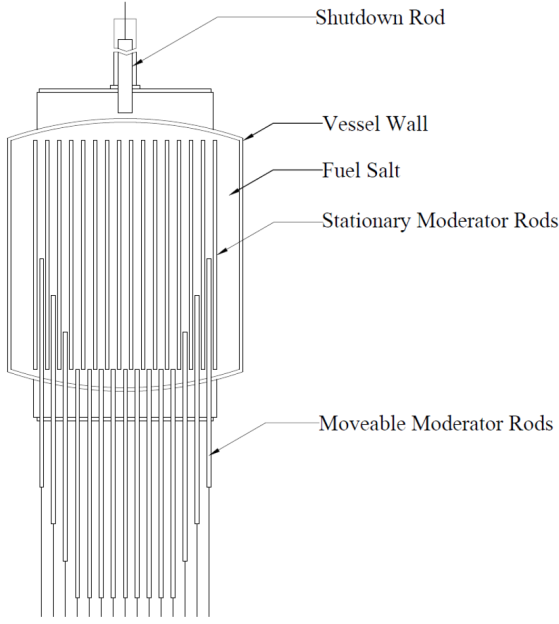
\includegraphics[width=0.65\textwidth]{tap_front_view.png}
	\caption{The \gls{TAP} \gls{MSR} schematic view showing movable moderator 
		rod 
		bundles and shutdown rod (figure reproduced from Transatomic Power 
		White Paper 
		\cite{transatomic_power_corporation_technical_2016}).}
	\label{fig:tap-main-view}
\end{figure}
The \gls{TAP} design (figure~\ref{fig:tap-main-view}) is very similar to 
original \gls{MSRE} design developed by \gls{ORNL} 
\cite{haubenreich_experience_1970} but has two major innovations: 
the fuel salt composition and the moderator. The \gls{MSRE}'s 
LiF-BeF$_2$-ZrF$_4$-UF$_4$ salt has been substituted with LiF-UF$_4$ salt 
which allows for an increase in the uranium concentration within the fuel salt 
from 0.9 to 27.5\% while maintaining a relatively low melting point 
(490$^{\circ}$C compared with 434$^{\circ}$C for the original \gls{MSRE}'s 
salt) \cite{betzler_two-dimensional_2017}. The graphite has a very high 
thermal scattering cross section which makes it a perfect moderator but has 
a few major drawbacks: 
(1) the low lethargy gain per collision requires a large volume of moderator 
to be present to reach criticality, which leads to a larger core and obstructs 
the core power density; (2) even special 
reactor-grade graphite has relatively high porosity, consequently, it holds
gaseous \glspl{FP} 
(e.g., tritium, xenon) in pores; (3) the reactor graphite lifespan in a 
commercial 
reactor is about 10 years \cite{robertson_conceptual_1971}. To resolve these 
issues, the \gls{TAP} concept uses another 
moderator, namely, zirconium hydride, allowing for a more compact core and a 
significant increase in power density. These two innovative design choices,  
together with a configurable moderator 
(the moderator-to-fuel ratio can be changed during regular maintenance 
shutdown), 
facilitate the commercial deployment of this conceptual design in the current 
commercially available 5\% \gls{LEU} fuel cycle. 

The \gls{TAP} \gls{MSR} primary loop contains the reactor core volume 
(including the zirconium hydride moderator rods with silicon carbide 
cladding), pumps, and primary heat exchanger. Pumps circulate the 
LiF-(Act)F$_4$ fuel salt through the primary loop. The pumps, vessels, tanks, 
and piping are made of a nickel-based alloy (similar to Hastelloy-N\footnote{ 
Hastelloy-N is very common in reactors now but have been studied and 
developed at \gls{ORNL} in a program that started in the 1950s.}), which is 
highly resistant to corrosion in various molten salt environments. Inside the 
reactor vessel, near the zirconium hydride moderator 
rods, the fuel salt is in a critical configuration and generates heat. 
Table~\ref{tab:tap_tab} contains details of the \gls{TAP} system 
design which are taken from technical white paper 
\cite{transatomic_power_corporation_technical_2016} 
and a neutronics overview
\cite{transatomic_power_corporation_neutronics_2016} as well as \gls{ORNL} 
analysis of the \gls{TAP} 
design \cite{betzler_two-dimensional_2017, betzler_assessment_2017}. 
%%%%%%%%%%%%%%%%%%%%%%%%%%%%%%%%%%%%%%%%
\begin{table}[h!]
	\caption{Summary of principal data for the \gls{TAP} \gls{MSR} 
		(reproduced from \cite{transatomic_power_corporation_technical_2016, 
		betzler_assessment_2017}). }
	\begin{tabularx}{\textwidth}{ s  s}
		\hline
		Thermal power				           		& 1250 MW$_{th}  $       
		\\ 
		Electric power		                		& 520 MW$_e  $ 			 
		\\ 
		Gross thermal efficiency        			& 44\%     				 
		\\  
		Outlet temperature							& 620$^{\circ}$C         
		\\ 
		Fuel salt components                   & LiF-UF$_4$				 \\  
		Fuel salt composition                  & 72.5-27.5 mole\%			 
		\\  
		Uranium enrichment                     & 5\% $^{235}$U          	 \\
		Moderator                              & Zirconium Hydride 
		(ZrH$_{1.66}$) rods (with silicon carbide cladding) \\
		Neutron spectrum						& 
		thermal/epithermal                 \\
		\hline
	\end{tabularx}
	\label{tab:tap_tab}
\end{table}
%%%%%%%%%%%%%%%%%%%%%%%%%%%%%%%%%%%%%%%%%%%%%%%%
\subsection{TAP core design}
In the \gls{TAP} core (figure~\ref{fig:tap-core-view}), fuel salt flows around 
moderator assemblies consisting of lattices of zirconium hydride rods clad in 
a corrosion-resistant silicone carbide (figure~\ref{fig:tap-main-view}). The 
\gls{TAP} reactor pressure vessel is a cylinder with an inner radius 150 cm, 
height 350 cm, and wall thickness 5 cm made of a nickel-based alloy. 
\begin{figure}[t] % replace 't' with 'b' to 
	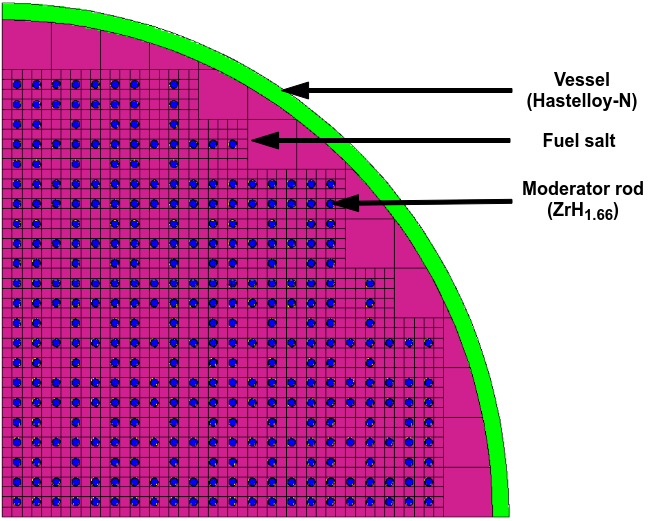
\includegraphics[width=\textwidth]{tap_core_ornl.png}
	\vspace{-0.35in}
	\caption{The \gls{TAP} \gls{MSR} schematic core view showing moderator 
		rods 
		(figure reproduced from ORNL/TM-2017/475  
		\cite{betzler_assessment_2017}).}
	\label{fig:tap-core-view}
\end{figure}

The \gls{SVF} in the core is parameter similar to wide-used moderator-to-fuel 
ratio and can be defined as:
\begin{align}
SVF &= \frac{V_F}{V_F+V_M} = \frac{1}{1+V_M/V_F}
\intertext{where}
V_F &= \mbox{the fuel volume} \nonumber \\
V_M &= \mbox{the moderator volume} \nonumber \\
V_M/V_F &= \mbox{the moderator-to-fuel salt ratio} \nonumber
\end{align}

The \gls{SVF} in the core can be varied during operation to shift the 
spectrum from intermediate to thermal energies (from \gls{BOL} to \gls{EOL}, 
respectively) to maximize fuel burnup. In practice, \gls{SVF} can be varied by 
inserting fixed-sized moderator rods via the bottom of the reactor vessel (for 
safety considerations), similarly to moving the control rods in a \gls{BWR}, 
as shown in Figure~\ref{fig:tap-main-view}. For the \gls{TAP} reactor, 
\gls{EOL} occurs when the maximum number of moderator rods are inserted into 
the core, and a further injection of fresh fuel salt does not change a 
criticality. Unmoderated salt is flowing in the annulus between the core, and 
the vessel wall provides for a potential reduction in fast neutron flux at the 
vessel structural material  
\cite{transatomic_power_corporation_neutronics_2016}.

\subsection{Serpent 2 full-core model} \label{sec:tap_model}
Advanced geometry surfaces and transformation capabilities of Serpent 
\cite{leppanen_serpent_2013} are employed to represent \gls{TAP} core. 
Figure~\ref{fig:tap-serpent-plan} shows the $XY$ section of whole-core
configuration at the expected reactor operational level when all
control rods are fully withdrawn. Figures~\ref{fig:tap-serpent-elev} and 
~\ref{fig:tap-serpent-elev-zoom} show a longitudinal section of the reactor. 
This model contains the moderator rods with silicon carbide cladding, pressure 
vessel, and inlet and outlet plena (Table~\ref{tab:tap_model_param}). Fuel 
salt flows around rectangular moderator assemblies consisting of lattices of 
small-diameter zirconium hydride rods in a corrosion-resistant material. The 
\gls{SVF} for model herein is 0.907268, which means the modeled core is 
under-moderated and has intermediate spectrum.
\begin{figure}[htp!] % replace 't' with 'b' to 
	\centering
	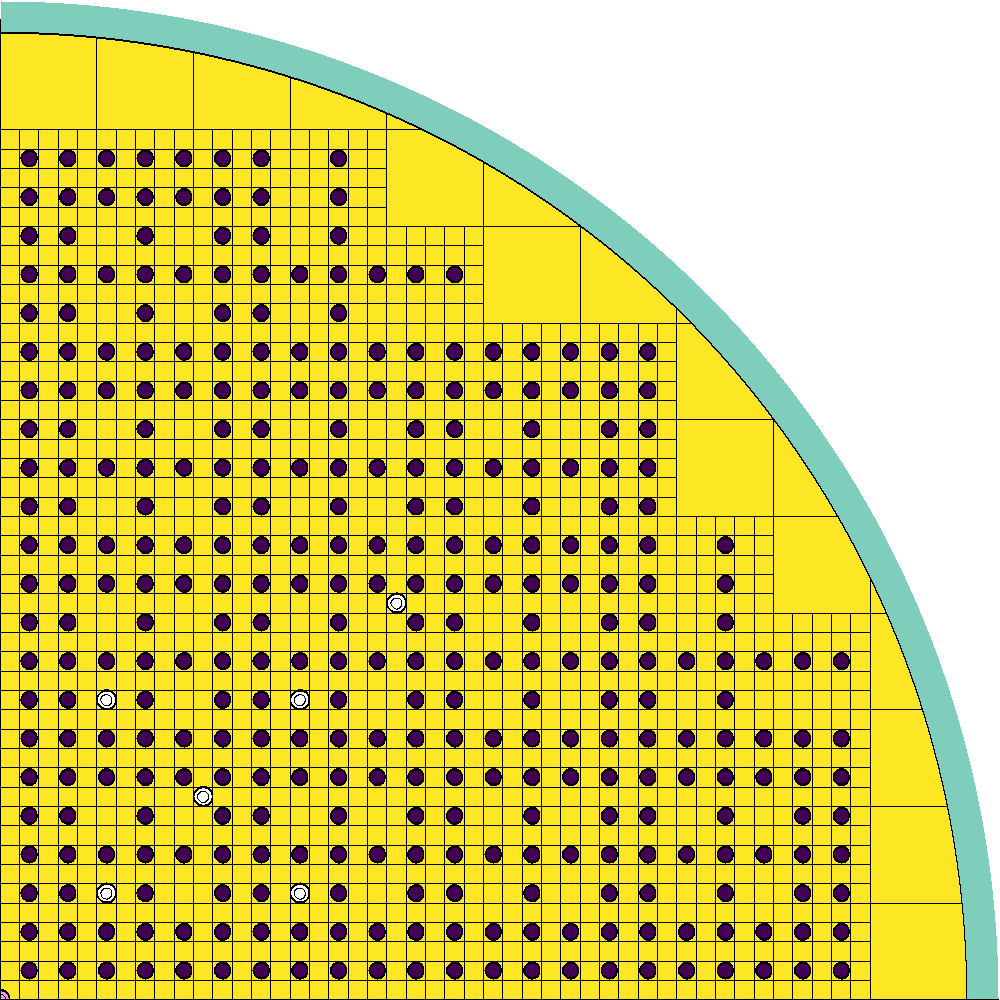
\includegraphics[width=\textwidth]{tap_plan_view.png}
	\caption{An $XY$ section of the \gls{TAP} model at horizontal midplane 
		with fully withdrawn control rods at \gls{BOL} (\gls{SVF}$=0.907268$). 
		The violet color represents zirconium 
		hydride, and the yellow represents fuel salt. The blue color shows 
		Hastelloy-N, a material used for the vessel wall, and the white color 
		is the air.}
	\label{fig:tap-serpent-plan}
\end{figure}
\begin{figure}[htp!] % replace 't' with 'b' to 
	\centering
	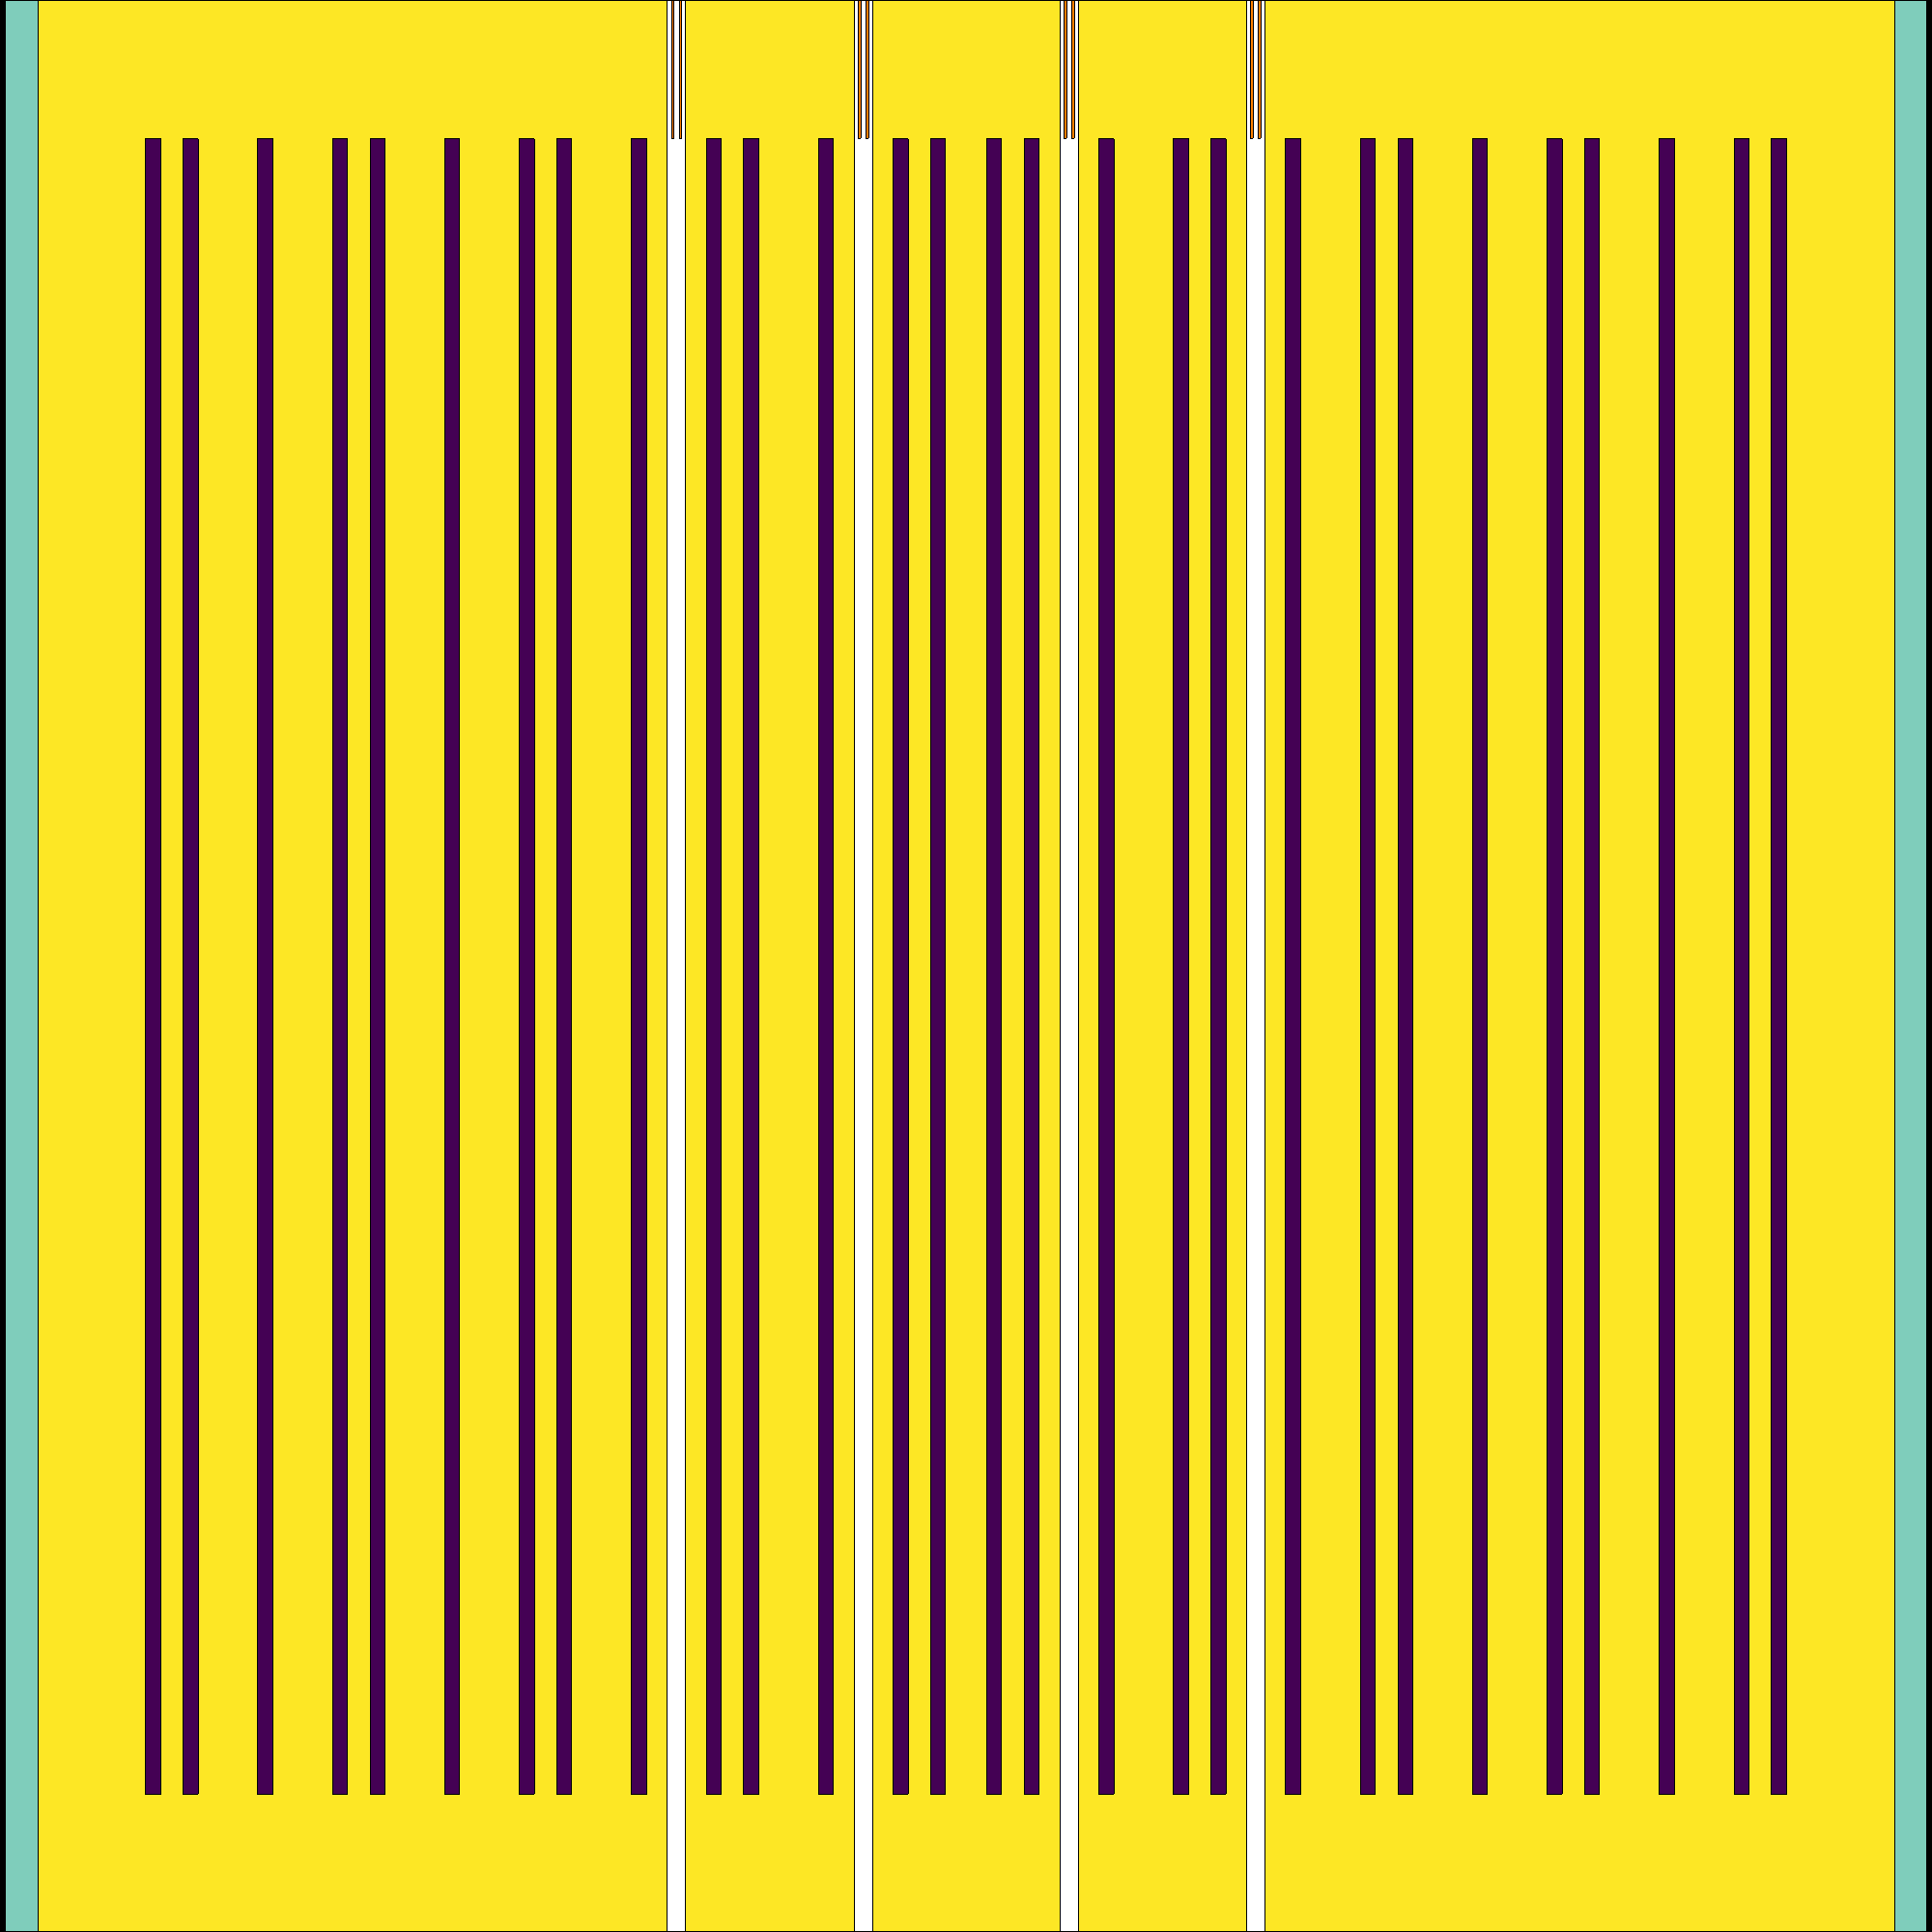
\includegraphics[width=\textwidth]{tap_elev_view.png}
	\caption{An $XZ$ section of the \gls{TAP} model.}
	\label{fig:tap-serpent-elev}
\end{figure}
\begin{figure}[htp!] % replace 't' with 'b' to 
	\centering
	\includegraphics[width=0.4\textwidth]{tap_elev_view_zoomed.png}
	\caption{Zoomed $XZ$ section of the top of the moderator rods and guide 
	tubes for \gls{TAP} model. The orange color shows 70-30\%  
	Gd$_2$O$_3$-Al$_2$O$_3$ ceramic absorbers used for control rods.}
	\label{fig:tap-serpent-elev-zoom}
\end{figure}

To represent reactivity control system, the model has: (1) control rod guide 
tubes made of nickel-based alloy; (2) control rods represented as hollow 
70-30\% Gd$_2$O$_3$-Al$_2$O$_3$ cylinders with a thin Hastelloy-N coating 
\cite{betzler_assessment_2017}; (3) air inside guide tubes and control rods. 
Control rods design has yielded a cluster of 25 rods that provide a total 
reactivity worth of $1121\pm26$pcm\footnote{ 1 pcm = 10$^{-5}\Delta 
k_{eff}/k_{eff}$.}.
%%%%%%%%%%%%%%%%%%%%%%%%%%%%%%%%%%%%%%%%%%%%%%%%%%
\begin{table}[hb!]
		\vspace{-0.2in}
	\caption{Geometric parameters for the full-core 3D model of the 
		\gls{TAP} (reproduced from Betzler \emph{et al.} 
		\cite{betzler_assessment_2017}). }
	\centering
	\begin{tabularx}{0.9\textwidth}{s s x p{0.14\textwidth}}
		\hline
		\textbf{Component} & \textbf{Parameter} & Value      		& 
		Unit		             \\ \hline
		\multirow{4}{*}{\begin{tabular}[c]{@{}l@{}}Moderator\\ 
				rod\end{tabular}} 
		& Cladding thickness      	  			    & 0.10 & cm				 
		\\  
		& Radius 				      	  			& 1.15 & cm				 
		\\  
		& Length				      	  			& 3.0  & m				 
		\\  
		& Pitch				      	  			& 3.0  & cm  			 \\ 
		\hline 
		
		\multirow{2}{*}{\begin{tabular}[c]{@{}l@{}}Moderator\\ 
				assembly\end{tabular}} 
		& Array				      	  			& 5 $\times$ 5 & 
		rods$\times$rods \\  
		& Pitch				      	  			& 15.0 & cm    				 
		\\  \hline
		
		\multirow{4}{*}{\begin{tabular}[c]{@{}l@{}}Core\end{tabular}}          
		& Assemblies  				   	  			& 268  & assemblies/core 
		\\  
		& Inner radius			      	  			& 1.5  & 
		m    				 \\  
		& Plenum height			   	  			& 25.0 & cm    				 
		\\  
		& Vessel wall thickness     	  			& 5.0 & 
		cm    				 \\ \hline            
	\end{tabularx}
	\label{tab:tap_model_param}
\end{table}
%%%%%%%%%%%%%%%%%%%%%%%%%%%%%%%%%%%%%%%%%%%%%%%%

The control rod cluster is modeled using the \textbf{TRANS} Serpent 2 feature, 
which allows easily to change the control rods position during the simulation. 
Herein I assumed that all control rods are fully withdrawn from the core 
(figure~\ref{fig:tap-serpent-elev-zoom}), but for future investigation control 
rods position may vary. In this report, all figures of the core were 
generated using the built-in Serpent plotter.

\section{TAP fuel salt reprocessing system}
The \gls{TAP} nuclear island contains \gls{FP} removal system. Gaseous  
\glspl{FP} are continuously removed using an off-gas system while liquid and 
solid \glspl{FP} are extracted via a chemical processing system. As these 
byproducts are gradually removed, a small quantity of fresh fuel salt is 
regularly added to the primary loop. This process conserves a constant fuel 
salt mass and keeps the reactor critical. In contrast with the \gls{MSBR} 
reprocessing system, the \gls{TAP} does not need a protactinium separation and 
isolation system because it operates in a uranium-based single-stage fuel 
cycle. The authors of the \gls{TAP} concept suggested three distinct fission 
product removal methods \cite{transatomic_power_corporation_neutronics_2016}:
\paragraph{Off-Gas System:} Removes gaseous fission products such as krypton 
and xenon, which are then compressed and stored temporarily until they have 
decayed to the background radiation level. Trace amounts of tritium are also 
removed and bottled in a liquid form via the same process. Also, the off-gas 
system directly removes a small fraction of the noble metals.
\paragraph{Metal Plate-Out/Filtration:} Removes noble and semi-noble metal 
solid fission products as they plate out onto a nickel mesh filter located in 
a side stream in the primary loop.
\paragraph{Liquid Metal Extraction:} Lanthanides and other non-noble metals 
stay dissolved in the fuel salt. They generally have a lower capture cross 
section and thus absorb fewer neutrons than $^{135}$Xe, but their extraction 
is essential to ensure normal operation. In the \gls{TAP} reactor, lanthanides 
removal is accomplished via a liquid-metal/molten salt extraction process 
similar to that developed for \gls{MSBR} by \gls{ORNL}  
\cite{robertson_conceptual_1971}. The process converts the dissolved 
lanthanides into a well-understood oxide waste form, similar to that of 
\gls{LWR} \gls{SNF}. This oxide waste comes out of the \gls{TAP} reprocessing 
plant in ceramic granules and can be sintered into another convenient form for 
storage.

Figure~\ref{fig:tap-reproc} shows a principal design of the \gls{TAP} primary 
loop, including an off-gas system, nickel mesh filter, and lanthanide chemical 
extraction facility. Similarly to \gls{MSBR}, an off-gas system is also based 
on a simple process of helium sparging through fuel salt with consequent gas 
bubbles removed before returning the fuel salt to the core. Nevertheless, 
one crucial difference must be noted: the \gls{MSBR} gas separation system 
suggested helium injection and subsequent transport of the voids throughout 
the primary loop, including the core for at least ten full loops 
\cite{robertson_conceptual_1971}. It is a significant concern to safe, stable 
operation because the increase of void fraction in the fuel salt when it 
enters back to the core would cause unpredictable reactivity change. This 
drawback can be overcome by using an effective gas separator for stripping 
helium/xenon bubbles before returning the salt to a primary loop 
(Figure~\ref{fig:tap-reproc}, blue block). 
\begin{figure}[htp!] % replace 't' with 'b' to 
	\centering
	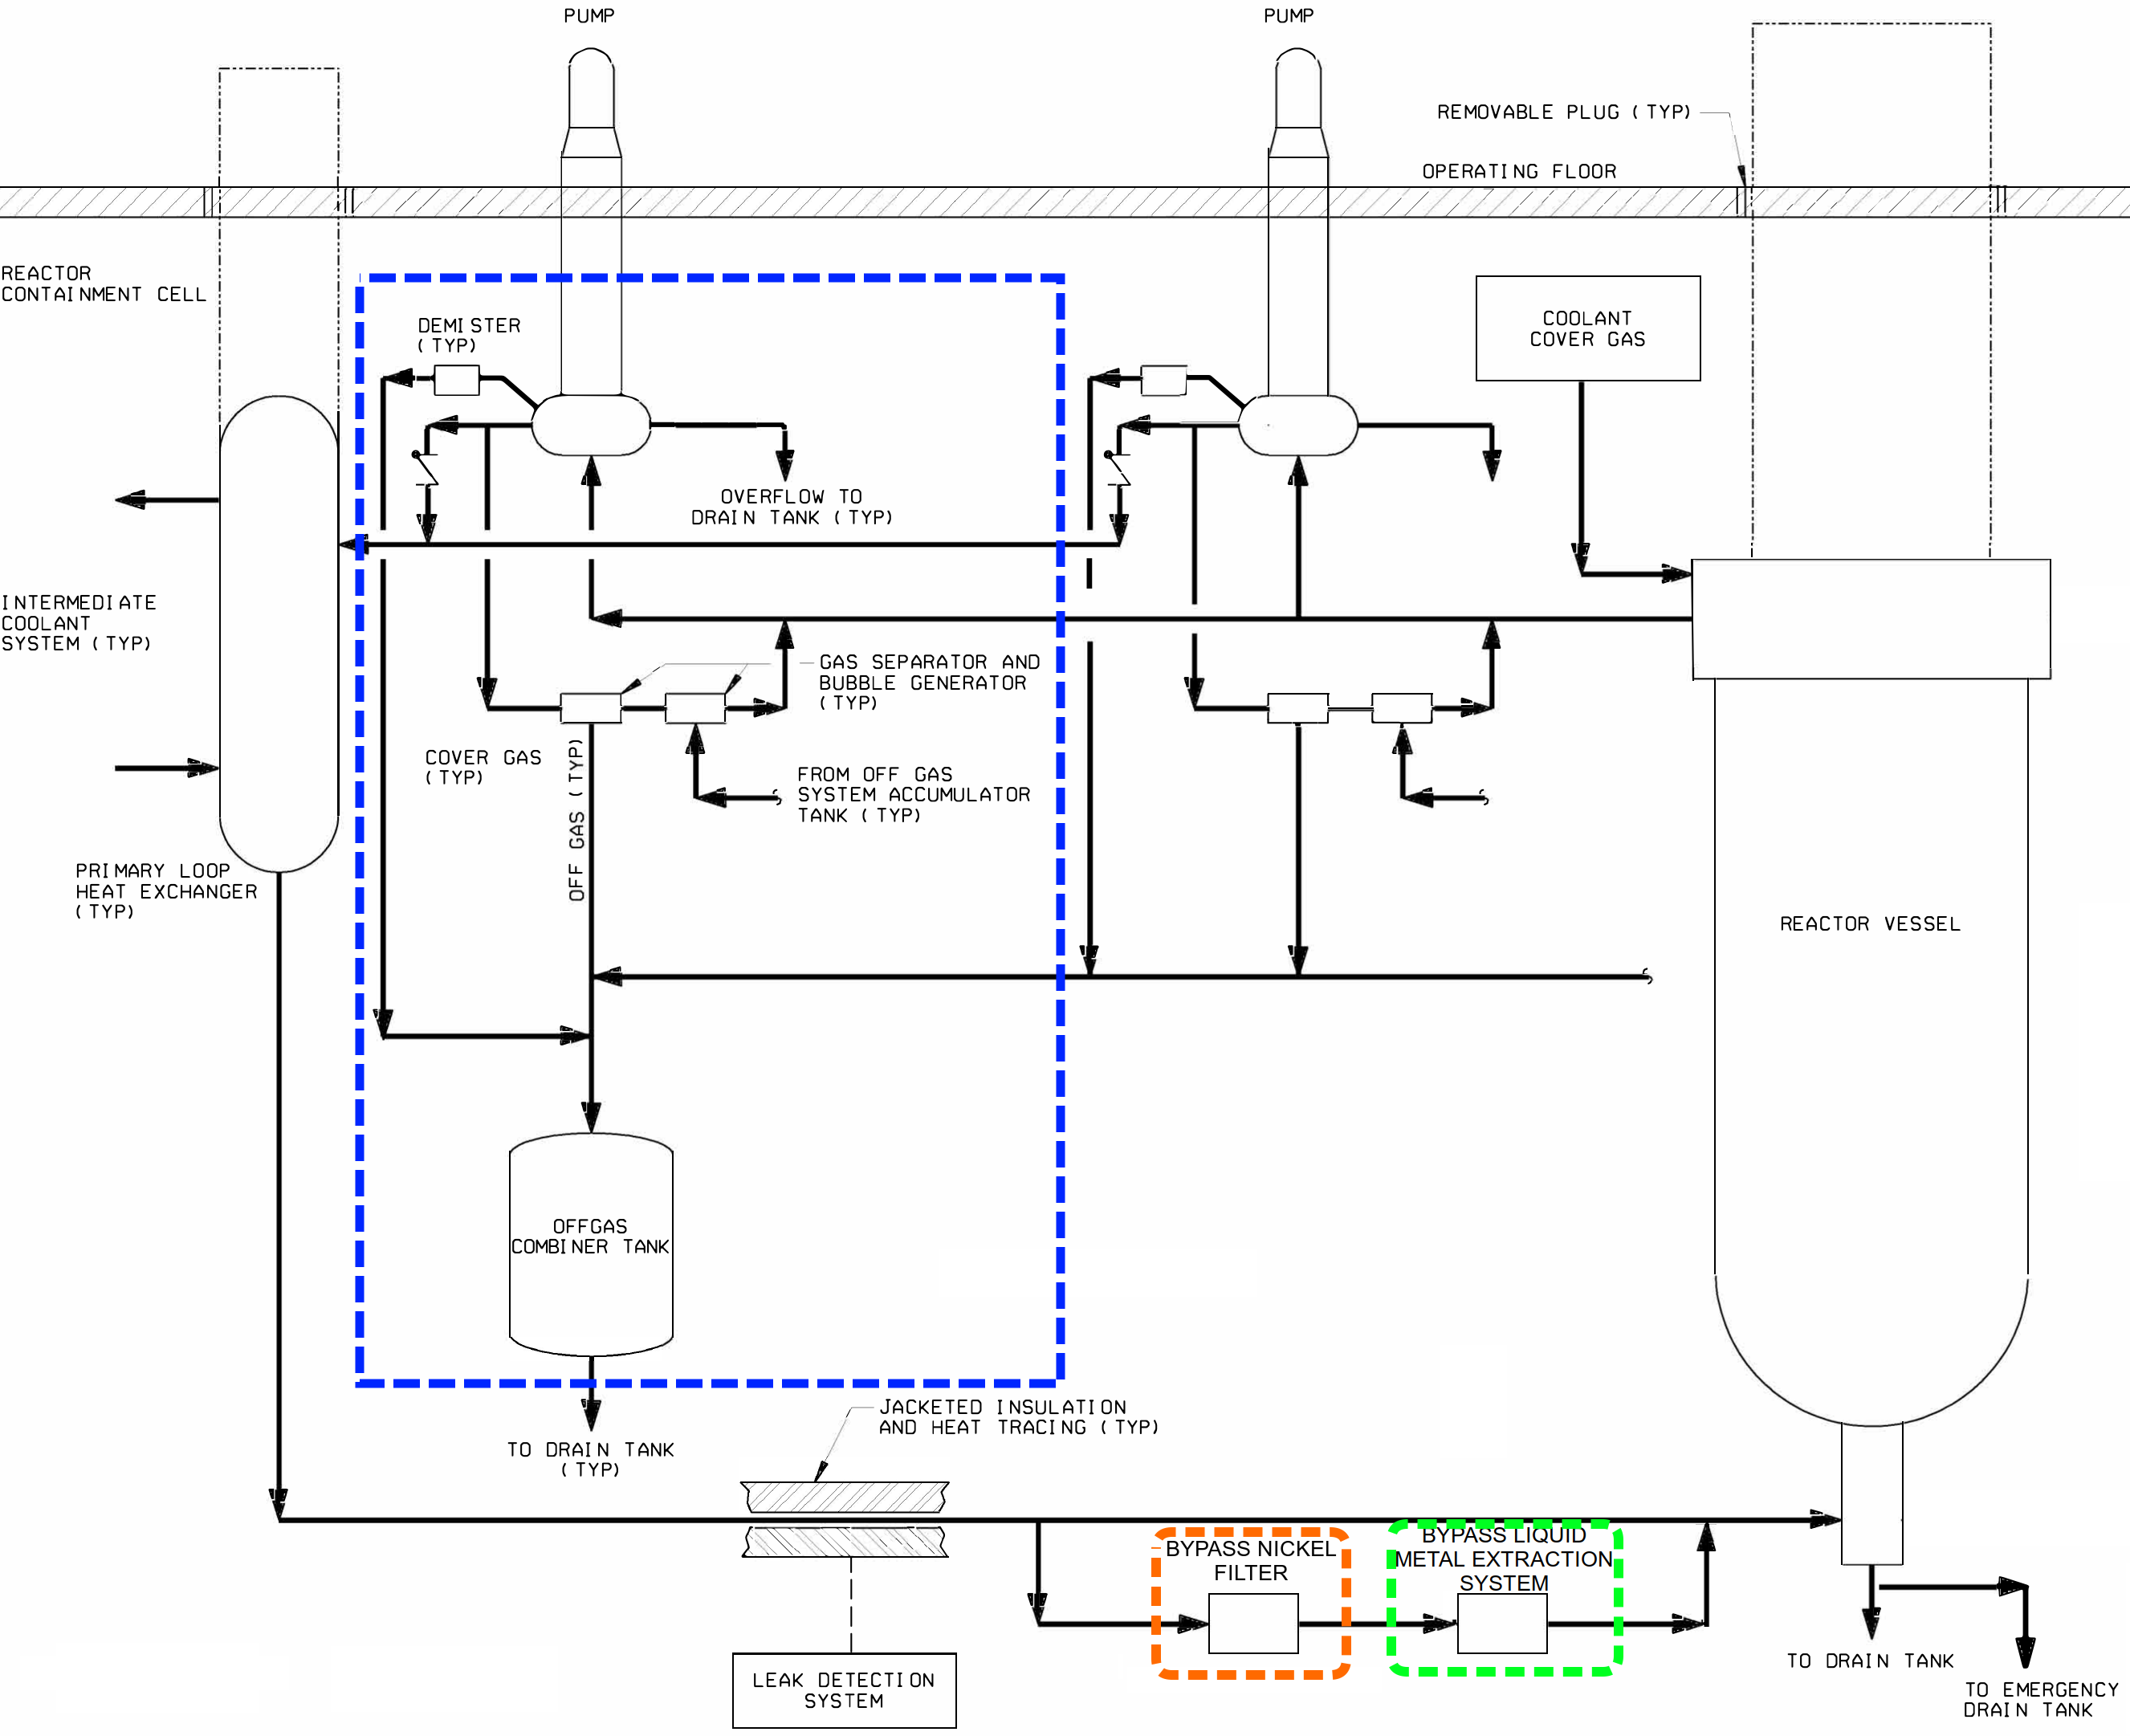
\includegraphics[width=\textwidth]{tap_primary_loop.png}
	\caption{Simplified \gls{TAP} primary loop design including off-gas system 
	(blue), 
		nickel filter (orange) and liquid metal extraction system (green) 
		(reproduced from \cite{transatomic_power_transatomic_2019}).}
	\label{fig:tap-reproc}
\end{figure}

Noble and semi-noble metal solid fission products tend to plate out onto metal 
surfaces including piping, heat exchanger tubes, reactor vessel inner surface, 
etc. Previous research by \gls{ORNL} \cite{robertson_conceptual_1971} reported 
that about 50\% of noble and semi-noble metals would plate out inside 
\gls{MSBR} systems without any special treatment. To improve the extraction 
efficiency of these fission products, the \gls{TAP} concept suggested 
employing a nickel mesh filter located in a bypass stream in the primary loop 
(Figure~\ref{fig:tap-reproc}, orange block). The main idea of this filter is 
to create a maze with large metal (nickel) surface area. The fuel salt is  
flowing throughout the filter and noble metals plate-out on the internal  
filter surface. 

This Liquid Metal Extraction process for the \gls{TAP} concept has been 
adopted from the \gls{MSBR}. The \gls{MSRE} demonstrated a liquid-liquid 
extraction process for removing rare earths and lanthanides from fuel salt and 
estimated efficiency of this process. Removal efficiency ($\epsilon_{RE}$) of  
this process is the function of salt mass flow rate, liquid bismuth mass 
flow rate, interfacial areas between salt and metal, and mass transfer 
coefficient for each noble metal species. The most recent research for LiF 
salt (for the \gls{MSFR} concept) reported the following form of extraction 
efficiency correlation \cite{rodrigues_actinide/lanthanide_2015}:
\begin{align} 
\epsilon_{RE} &= \frac{1}{1+10^{\lambda}} \nonumber \\
&= \frac{1}{1+10^{f(A, \dot{m}_{Bi}, \dot{m}_{salt}, N, K)}} \label{eq:re_eff}
\intertext{where}
A&= \mbox{metal-to-salt interface area} \nonumber \\
\dot{m}_{Bi}&= \mbox{bismuth mass flow rate} \nonumber \\
\dot{m}_{salt}&= \mbox{salt mass flow rate} \nonumber \\
N&= \mbox{number of stages} \nonumber \\
K&= \mbox{liquid phase mass transfer coe cient} \nonumber 
\end{align}
Correlations are different for various lanthanides and can be determined from 
experimental data and/or existing analytical models 
\cite{mcneese_engineering_1971, delpech_possible_2012, 
rodrigues_actinide/lanthanide_2015}.

In fact, due to similarities in reprocessing schemes, the \gls{TAP} project 
reported almost the same set of elements for removal and similar effective 
cycle times as suggested for \gls{MSBR} (Table~\ref{tab:reprocessing_list}). 
The \gls{TAP} neutronics whitepaper specifies additional low-probability 
fission products and gases that should be removed during operation. These 
elements are categorized into the previously defined processing groups, but 
the removal rates of most of these elements (i.e., all except for hydrogen) 
are very low.
%%%%%%%%%%%%%%%%%%%%%%%%%%%%%%%%%%%%%%%%
\begin{table}[ht!]
	\centering
	\caption{The effective cycle times for fission products removal  from the 
	\gls{TAP} reactor (reproduced from \cite{betzler_implementation_2017} and 
	\cite{transatomic_power_corporation_neutronics_2016}).}
	\begin{tabular}{p{0.2\textwidth} p{0.42\textwidth} p{0.12\textwidth} 
	p{0.16\textwidth}}
		\hline 
		%\begin{tabularx}{\linewidth}{l X} \toprule 
		Processing group & \qquad\qquad\qquad Nuclides & Removal Rate 
		(s$^{-1}$) & Cycle time (at full power) \\ [5pt] \hline 
		\multicolumn{3}{c}{\textit{Elements removed in \gls{MSBR} concept and 
		adopted for the \gls{TAP}} \cite{robertson_conceptual_1971}} \\
		Volatile gases & Xe, Kr								  & 5.00E-2 & 20 
		sec \\ [5pt]
		Noble metals & Se, Nb, Mo, Tc, Ru, Rh, Pd, Ag, Sb, Te & 5.00E-2 & 20 
		sec \\ [5pt]
		Seminoble metals & Zr, Cd, In, Sn	  				  & 5.79E-8 & 200 
		days \\ [5pt]
		Volatile fluorides & Br, I 							  & 1.93E-7 & 60 
		days \\ [5pt]
		Rare earths & Y, La, Ce, Pr, Nd, Pm, Sm, Gd           & 2.31E-7 & 50 
		days \\ [5pt]
		\qquad & Eu & 2.32E-8 & 500 days \\ [5pt]
		Discard & Rb, Sr, Cs, Ba & 3.37E-9 & 3435 days \\ [5pt] 
		\hline
		
		\multicolumn{3}{c}{\textit{Additional elements removed} 
		\cite{transatomic_power_corporation_neutronics_2016, 
		betzler_implementation_2017}  } \\
		Volatile gases & H								  	& 5.00E-2 & 20 
		sec    \\ [5pt]
		Noble metals & Ti, V, Cr, Cu						& 3.37E-9 & 3435 
		days \\ [5pt]
		Seminoble metals & Mn, Fe, Co, Ni, Zn, Ga, Ge, As   & 3.37E-9 & 3435 
		days \\ [5pt]
		Rare earths & Sc									& 3.37E-9 & 3435 
		days \\ [5pt]
		Discard & Ca										& 3.37E-9 & 3435 
		days \\ [5pt] 
		\hline
	\end{tabular}
	\label{tab:reprocessing_list}
	\vspace{-0.9em}
\end{table}
Details of gas removal and fuel reprocessing systems have historically 
been conceptual and liquid-fueled system designers including the \gls{TAP} 
usually assumed ideal (rather than realistically constrained) removal 
efficiencies for reactor performance simulations. For the  proposed work, the 
realistic online reprocessing system and reactor model will be created to 
capture the dynamics of fuel composition evolution during reactor operation. 
Gases removal efficiency will be represented in that model as a variable, 
described using mathematical correlation from Chapter 2 
(see Equation~\ref{eq:gas_eff}). For the other \glspl{FP}, a  
fixed\footnote{Published information about dynamics of extraction efficiency 
during reactor operation for seminoble metals, volatile fluorides, and rare 
earths is insufficient to inform a variable removal efficiency.}, non-ideal 
extraction efficiency based on cycle time from the  
table~\ref{tab:reprocessing_list} will be used in the fuel reprocessing model.

\section{Preliminary results} \label{sec:stage2-demo}
\subsection{TAP long-term demonstration case} 
I thoroughly analyzed the original \gls{TAP} reprocessing system design 
(figure~\ref{fig:tap-reproc}) and neutron poisons removal rates  
(table~\ref{tab:reprocessing_list}) to determine suitable reprocessing 
scheme for SaltProc v2.0+ demonstration (figure~\ref{fig:demo-repro-scheme}). 
That demonstration case assumed fixed, non-ideal ($<100$\%) removal 
efficiencies and static geometry with constant \gls{SVF} during 13 years of 
operation.
\begin{figure}[htp!] % replace 't' with 'b' to 
	\centering
	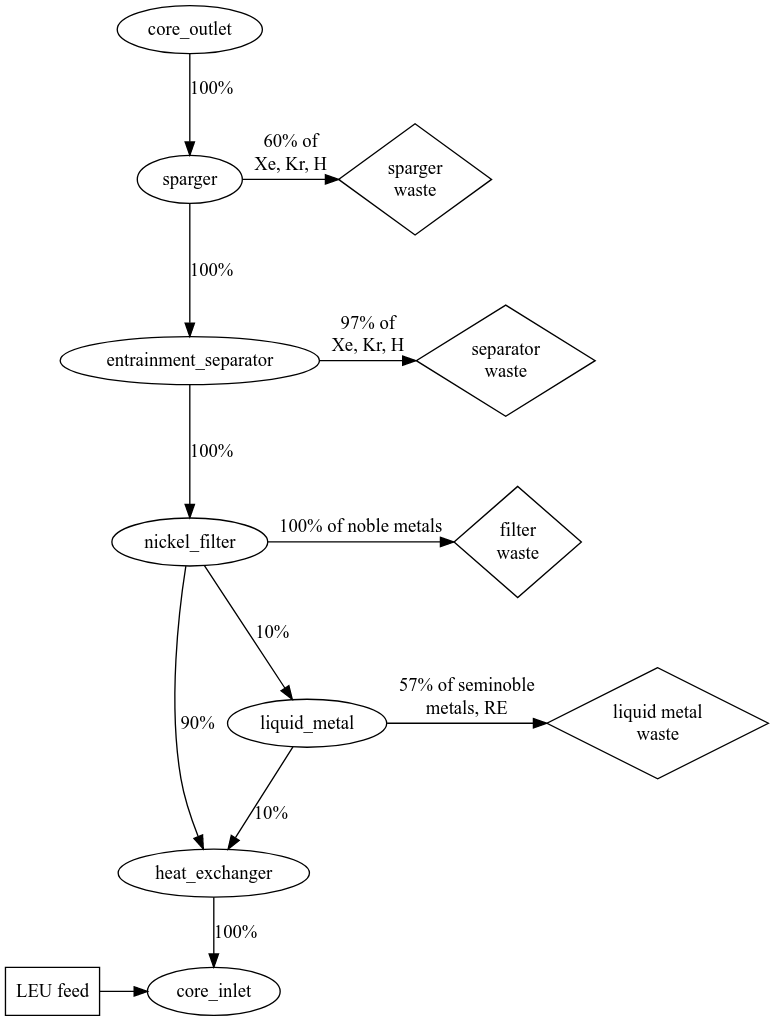
\includegraphics[width=0.93\textwidth]{demo_reprocessing_scheme.png}
	\caption{\gls{TAP} reprocessing scheme flowchart used for SaltProc v2.0+ 
		demonstration. Arrows represent material flows; percents - fraction of 
		total mass flow rate; ellipses - fuel reprocessing system components; 
		diamonds - waste streams; box shows refuel material flow.}
	\label{fig:demo-repro-scheme}
\end{figure}

The gas removal components (the sparger and entrainment separator) are located 
in-line because estimated full loop time for the fuel salt is about 
18 sec and approximately equal cycle time (table~\ref{tab:reprocessing_list}). 
To remove all volatile gases every 20 sec the fuel reprocessing system must 
operate with 100\% of the core throughout flow rate and exceptional 
efficiency. For the demonstration case herein to achieve required cycle time, 
I assumed that xenon, krypton, and hydrogen extraction efficiencies for the 
sparger and entrainment separator are equal to 60\% and 97\%, respectively.

The nickel filter in the \gls{TAP} concept is designed to extract noble metals 
and volatile fluorides. Similarly to volatile gases, noble metals must be 
removed every 20 sec and, hence, the filter should operate in-line also. The 
nickel filter removes a wide range of elements with various efficiencies 
(table~\ref{tab:reprocessing_list}).

Lanthanides and other non-noble metals generally have a lower capture  
cross-section and absorb fewer neutrons than gases and noble metals. These 
elements can be removed via a liquid-metal/molten salt extraction process with 
relatively low removal rates (cycle time $> 50$ days). This is accomplished 
using small fuel salt flow rate (10\% of the core throughout flow rate) via 
liquid-metal/molten salt component, where lanthanides are removed with 
specific extraction efficiency to match required cycle time  
(table~\ref{tab:reprocessing_list}). The rest 90\% of the flow is directed 
from the nickel filter to heat exchanger without performing any fuel salt 
treatment.

The removal rates vary among nuclides in this reactor concept, which dictate 
the necessary resolution of depletion calculations. To compromise, a 3-day 
time was selected based on Betzler \emph{et al.} timestep refinement study 
\cite{betzler_assessment_2017}.
\subsection{Effective multiplication factor}
Figures~\ref{fig:keff}, \ref{fig:keff-zoomed}, \ref{fig:keff-zoomed-2} 
demonstrate 
the effective 
multiplication factors  obtained using SaltProc v2.0+ and Serpent. I obtained 
the effective multiplication factors after removing fission products 
and adding feed material at the end of each depletion step (3 days for this 
work). The $k_{eff}$ fluctuates significantly as a result of the batch-wise 
nature of used online reprocessing strategy.
\begin{figure}[htp!] % replace 't' with 'b' to 
	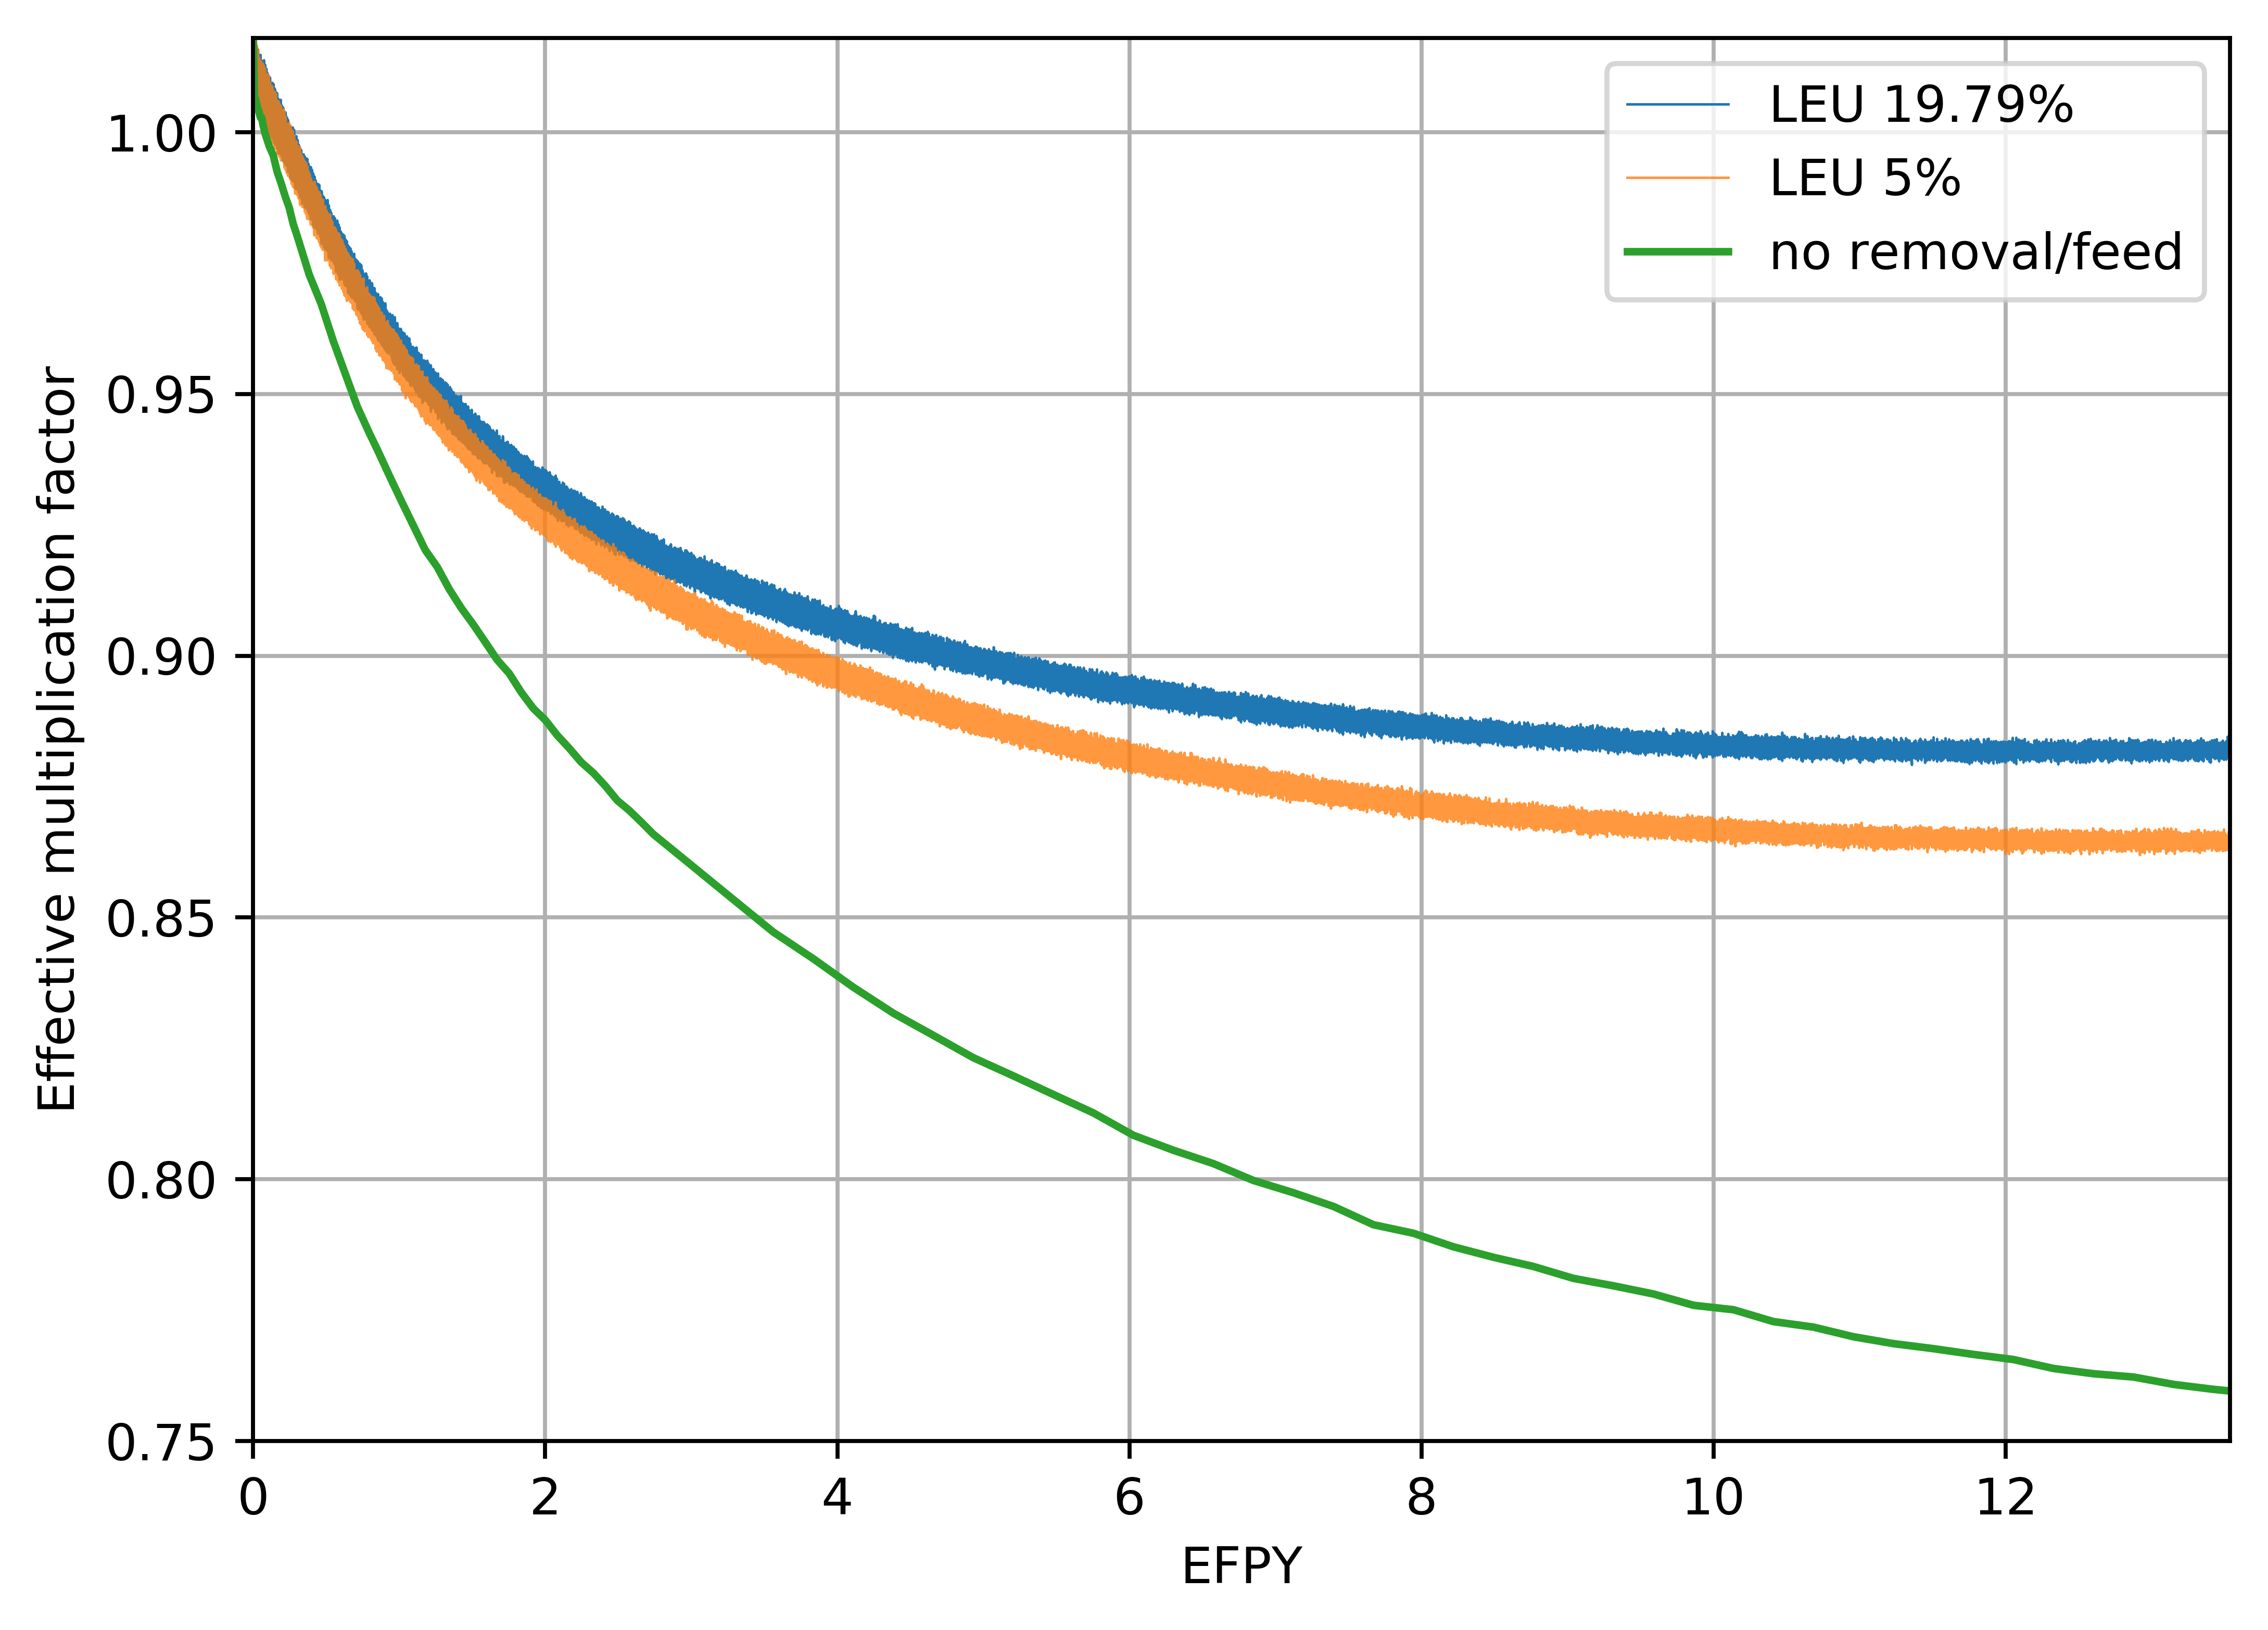
\includegraphics[width=\textwidth]{keff_3.png}
	\vspace{-0.2in}
	\caption{Effective multiplication factor dynamics for full-core
		\gls{TAP} model for different fueling scenarios over a 13-year reactor 
		operation. 
		Confidence interval $\pm\sigma=28pcm$ is shaded.}
	\label{fig:keff}
\end{figure}
\begin{figure}[htp!] % replace 't' with 'b' to 
	\centering
	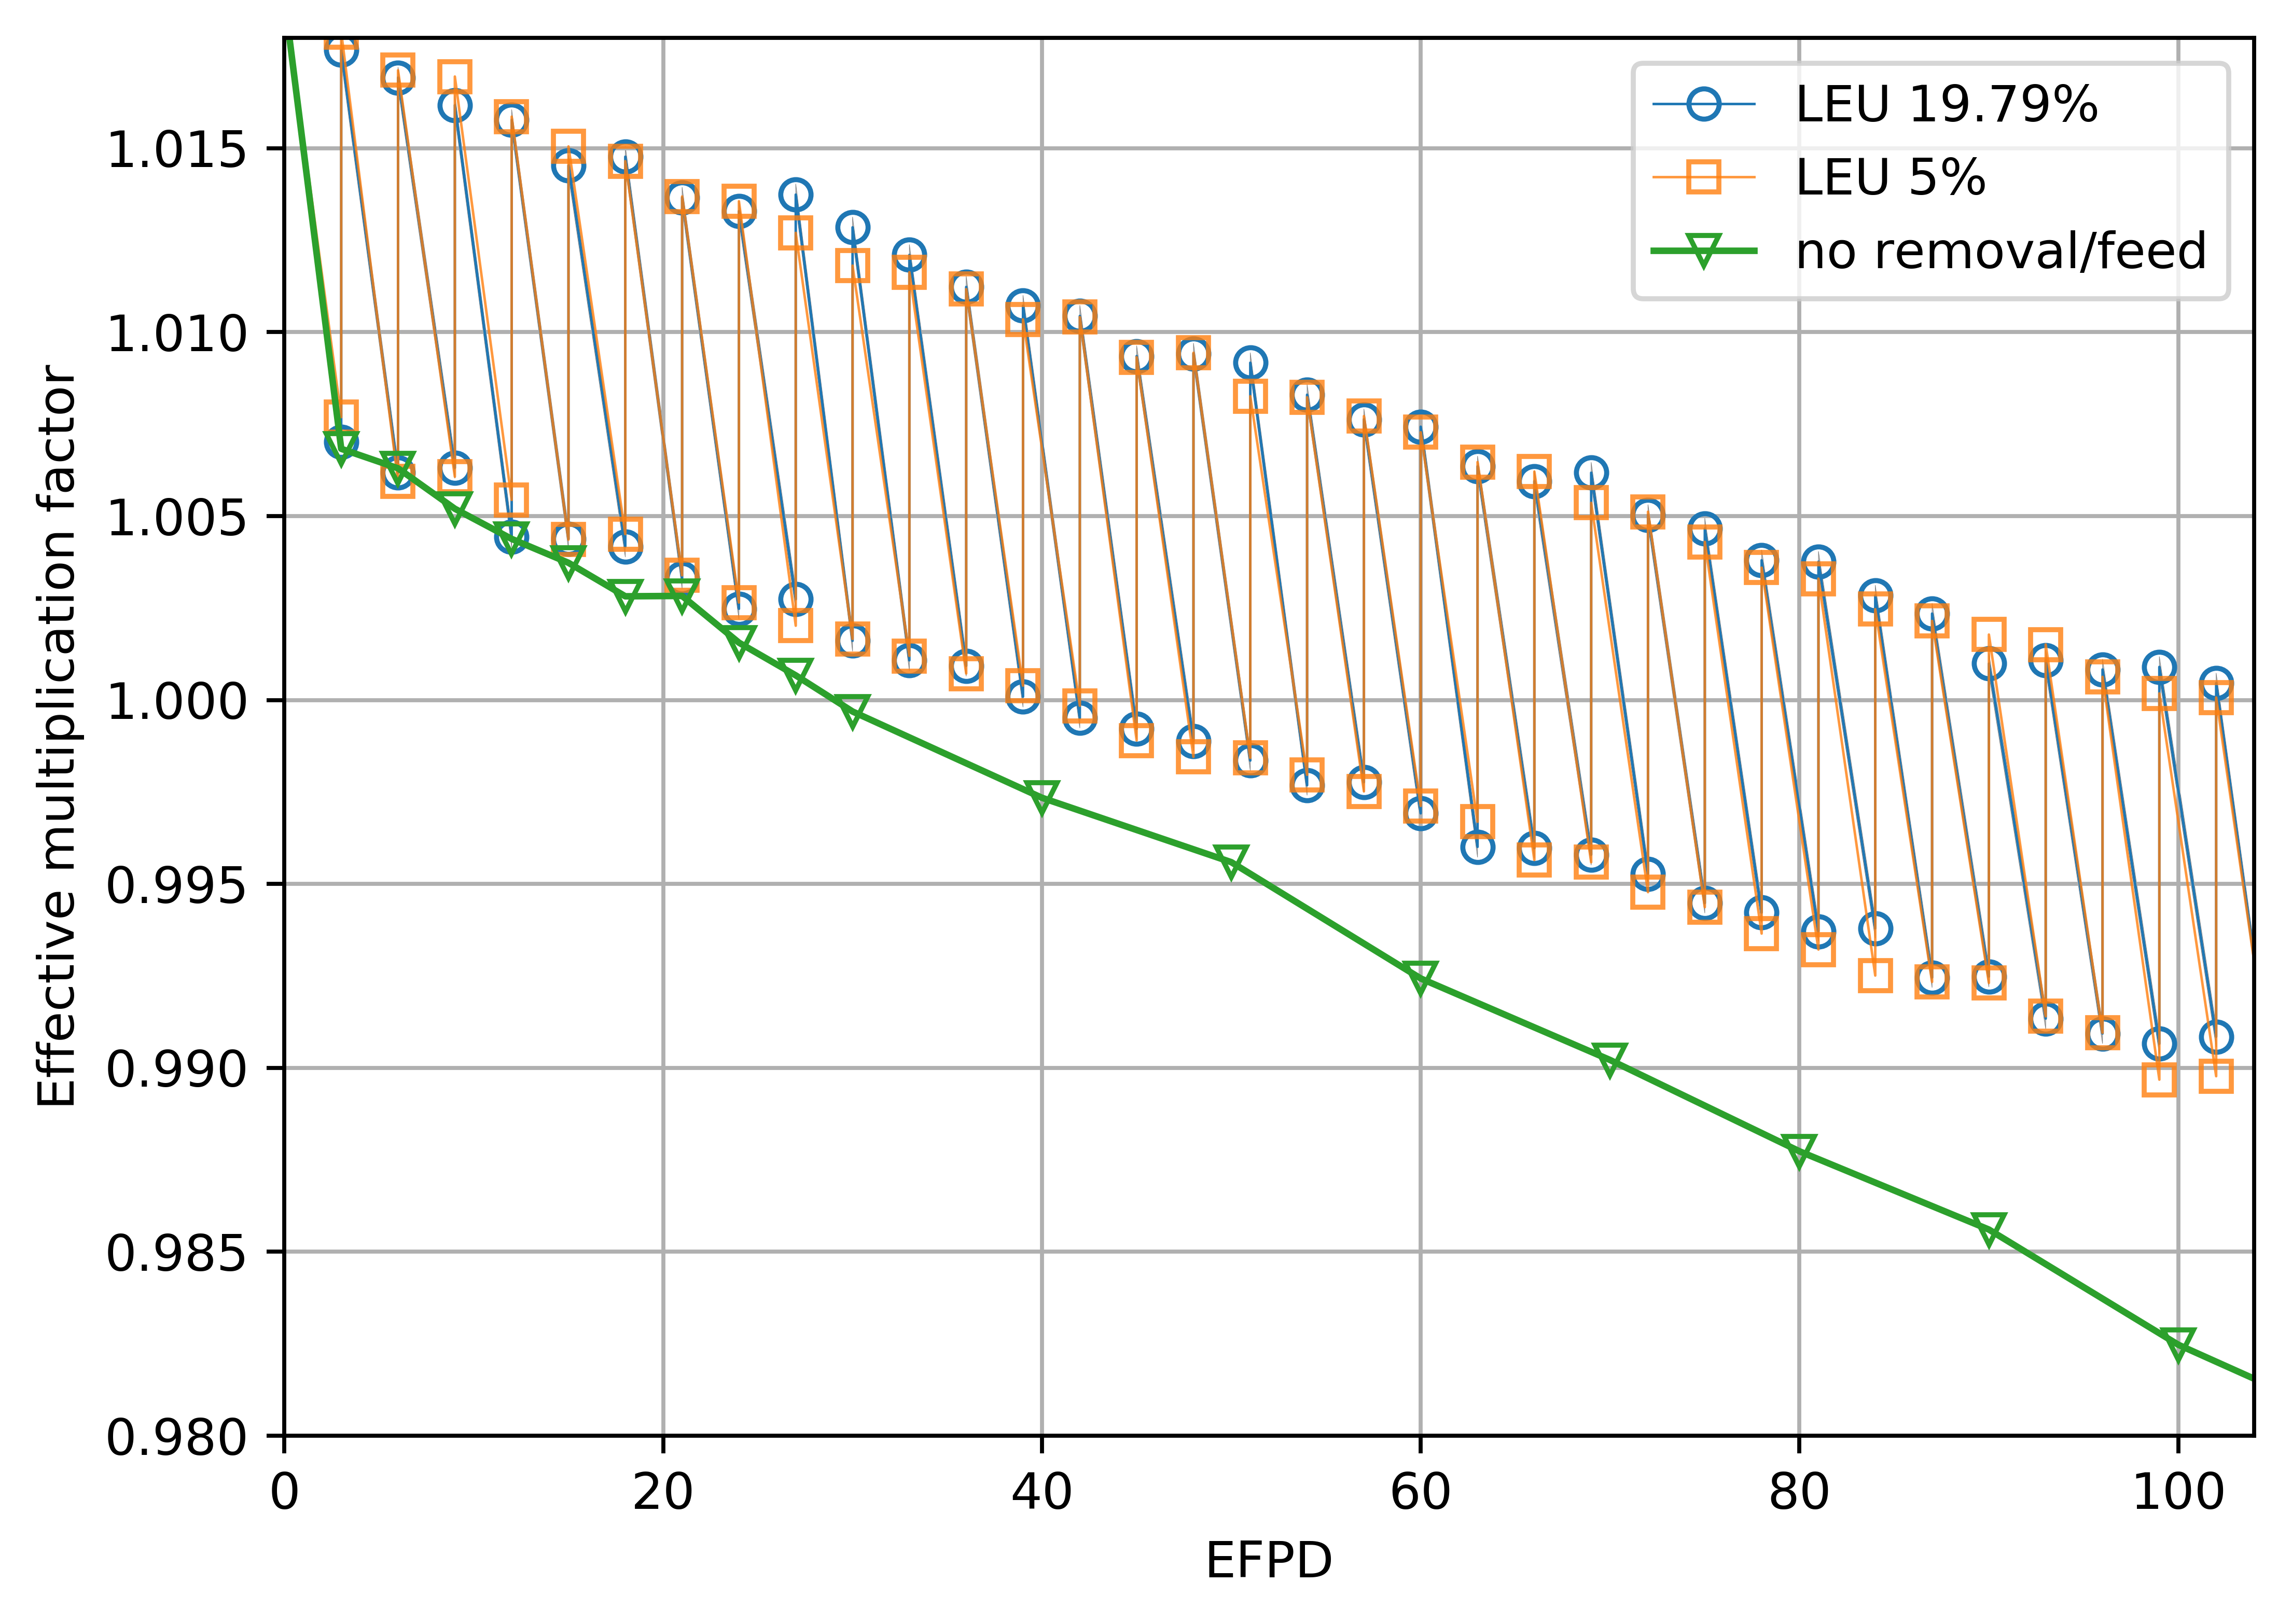
\includegraphics[width=0.85\textwidth]{keff_zoomed_1.png}
	\caption{Zoomed effective multiplication factor for the first 104 EFPD 
		after startup.}
	\label{fig:keff-zoomed}
\end{figure}
\begin{figure}[htp!] % replace 't' with 'b' to 
	\centering
	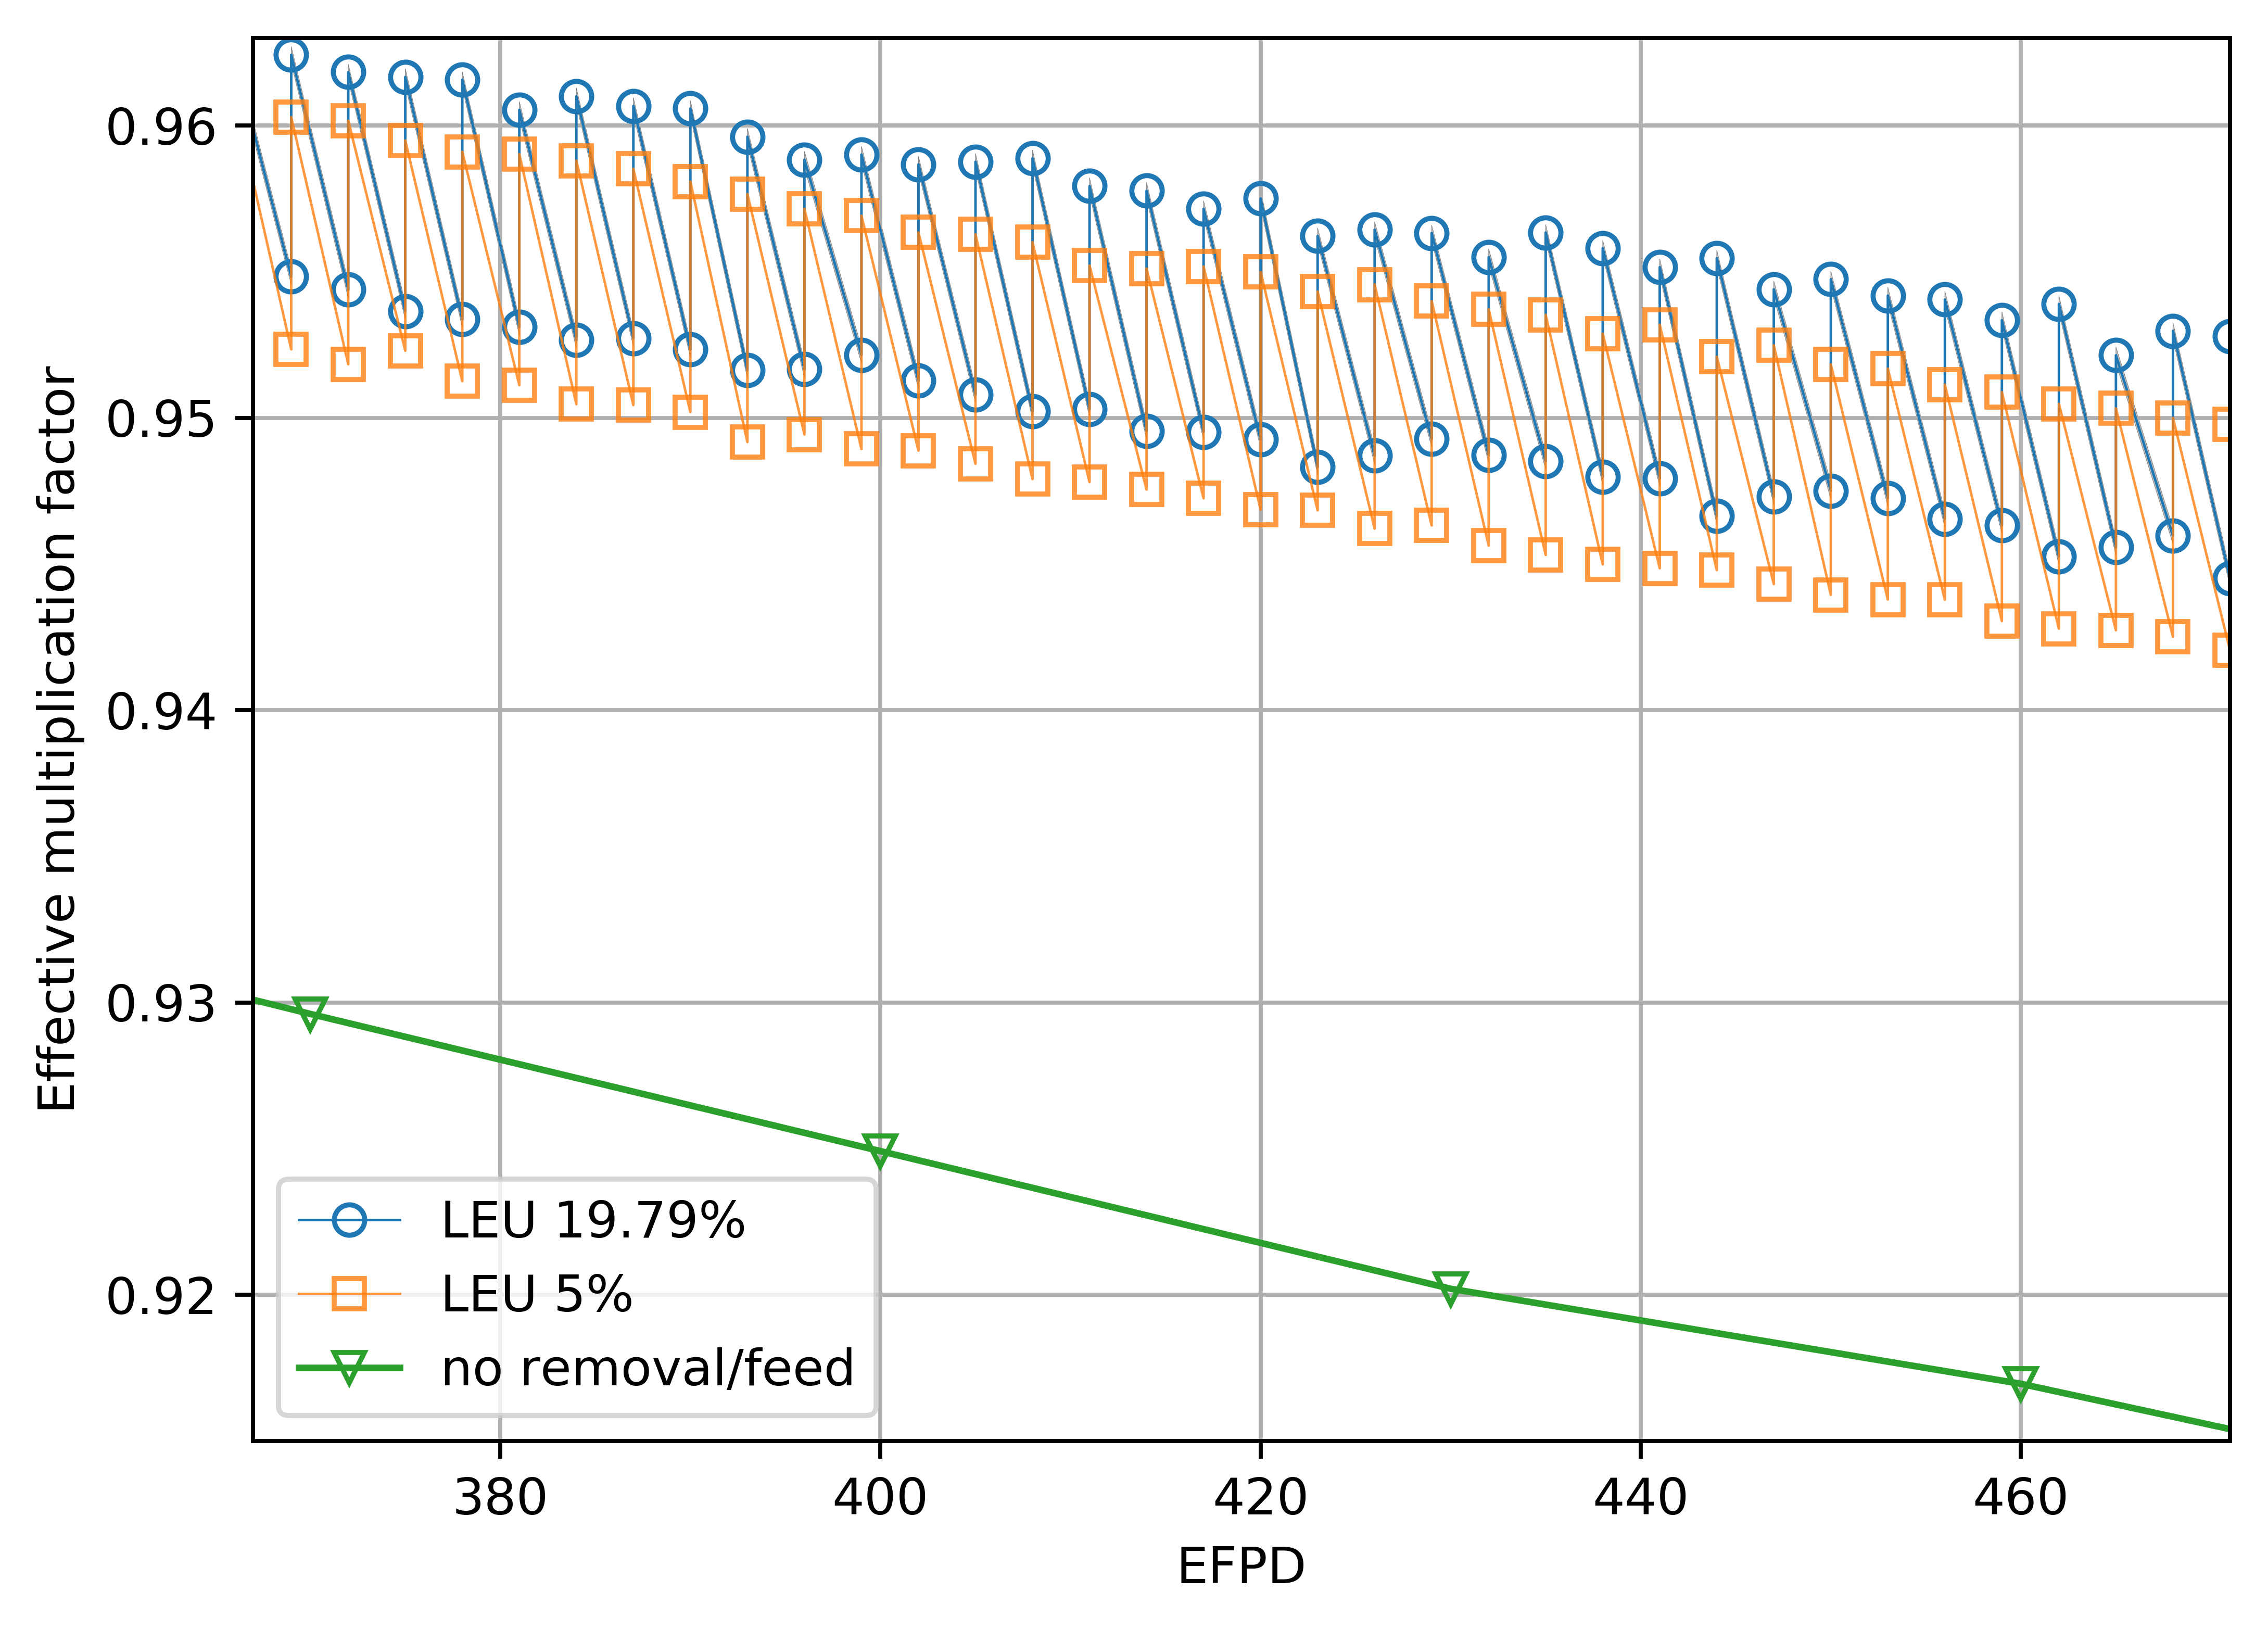
\includegraphics[width=0.85\textwidth]{keff_zoomed_2.png}
	\caption{Zoomed effective multiplication factor for the time interval 
		from 367 to 471 EFPD after startup.}
	\label{fig:keff-zoomed-2}
\end{figure}

Loading initial fuel salt composition with 5\% \gls{LEU} into the \gls{TAP} 
core leads to a supercritical configuration with an excess of reactivity about 
1900pcm (figure~\ref{fig:keff}). Without performing any fuel salt reprocessing 
the core became subcritical after 30 days of operation 
(figure~\ref{fig:keff-zoomed}). I obtained this result using naked Serpent 
without introducing any \gls{FP} extraction and refueling. For the beginning 
of the \gls{TAP} lifetime uranium enrichment in the feed has a minor effect 
because a tiny amount of poisons was produced ($<$1kg/day) and, hence, a small 
mass of fresh salt was injected. Notably, the core went subcritical after 42 
days of operation either with \gls{LEU} 5\% or \gls{LEU} 19.79\% feed.

The \gls{TAP} core is never reached equilibrium fuel salt composition without 
performing fuel salt reprocessing and refueling. For the fueling scenarios 
with 5\% and 19.79\% \gls{LEU} feed, the reactor achieved the equilibrium 
state after 10 years of operation. Overall, the effective multiplication 
factor gradually decreases from 1.018 to 0.88 for the 19.79\% \gls{LEU} feed 
and 0.86 for the 5\% \gls{LEU} feed, which indicates problems with operating 
this nuclear reactor design. I will try to overcome this issue by adding 
dynamic \gls{SVF} functionality to SaltProc v2.0+.

\subsection{Neutron spectrum}
Figure~\ref{fig:spectrum} shows the normalized neutron flux spectrum for the 
full-core \gls{TAP} core model in the energy range from 10$^{-8}$ to 15 MeV. 
The neutron energy spectrum at equilibrium is a little bit harder than at 
startup due to plutonium and other strong absorbers accumulating in the 
core during reactor operation. The \gls{TAP} spectrum is significantly 
harder than in a typical \gls{LWR} and is in a good agreement with 
\gls{ORNL} report \cite{betzler_assessment_2017}.
\begin{figure}[htp!] % replace 't' with 'b' to 
	\centering
	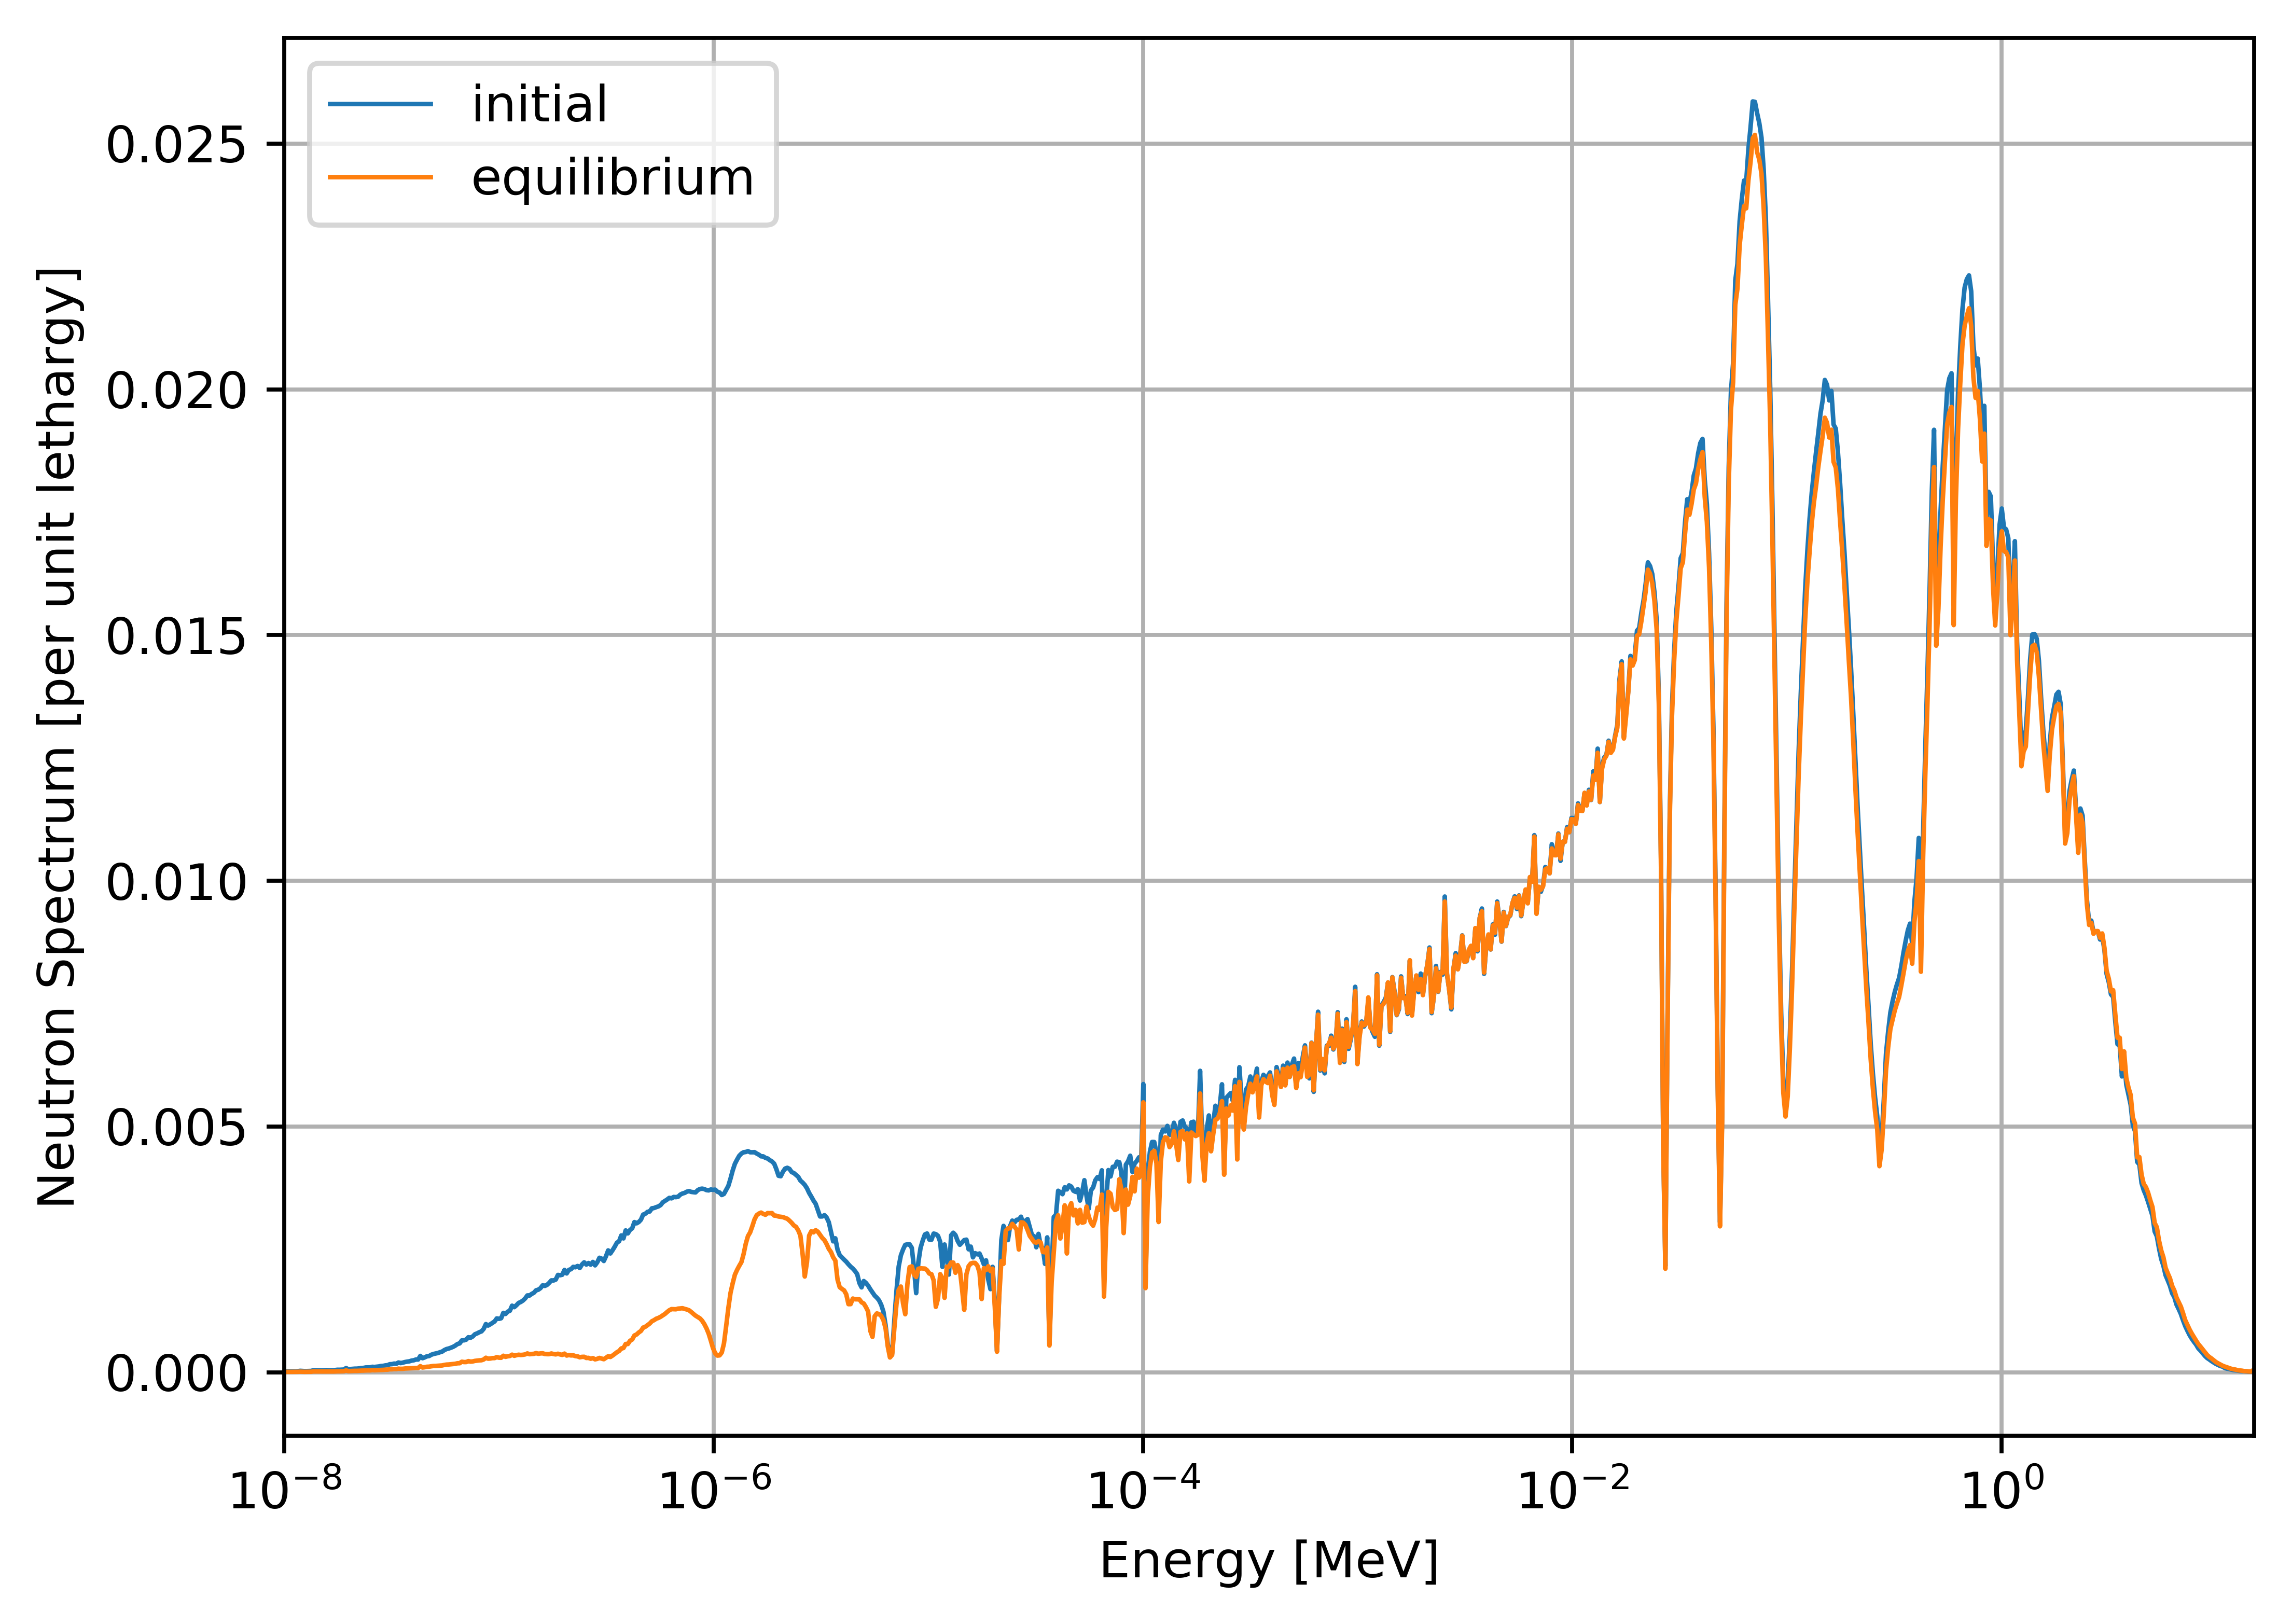
\includegraphics[width=\textwidth]{spectrum.png}
	\caption{The neutron flux energy spectrum normalized by unit lethargy 
		for initial and equilibrium fuel salt composition.}
	\label{fig:spectrum}
\end{figure}
\subsection{Fuel salt composition}
Figure~\ref{fig:u-pu} shows the absolute mass of major heavy isotopes 
which have a strong influence on the reactor core physics. The mass of 
$^{236}$U, $^{238}$U, $^{239}$Pu, $^{240}$Pu, and $^{241}$Pu in the 
fuel salt changes insignificantly after approximately 10 years of operation,
which matches stabilization time for effective multiplication factor. 
Hence, the quasi-equilibrium state was reached after 10 years of reactor 
operation. Moreover, the \gls{TAP} core bred approximately the same amount 
of fissile $^{239}$Pu ($\approx2$t) as was initial fissile material 
($^{235}$U) load. A significant amount of non-fissile plutonium builds 
up during operation and accounts for 50\% of the plutonium after 13 years 
of operation. Overall, rate of breeding fissile $^{239}$Pu from $^{238}$U 
even in relatively hard neutron spectrum is not large enough to compensate 
negative effects of strong absorbers accumulation and keep the reactor 
critical.
\begin{figure}[htp!] % replace 't' with 'b' to 
	\centering
	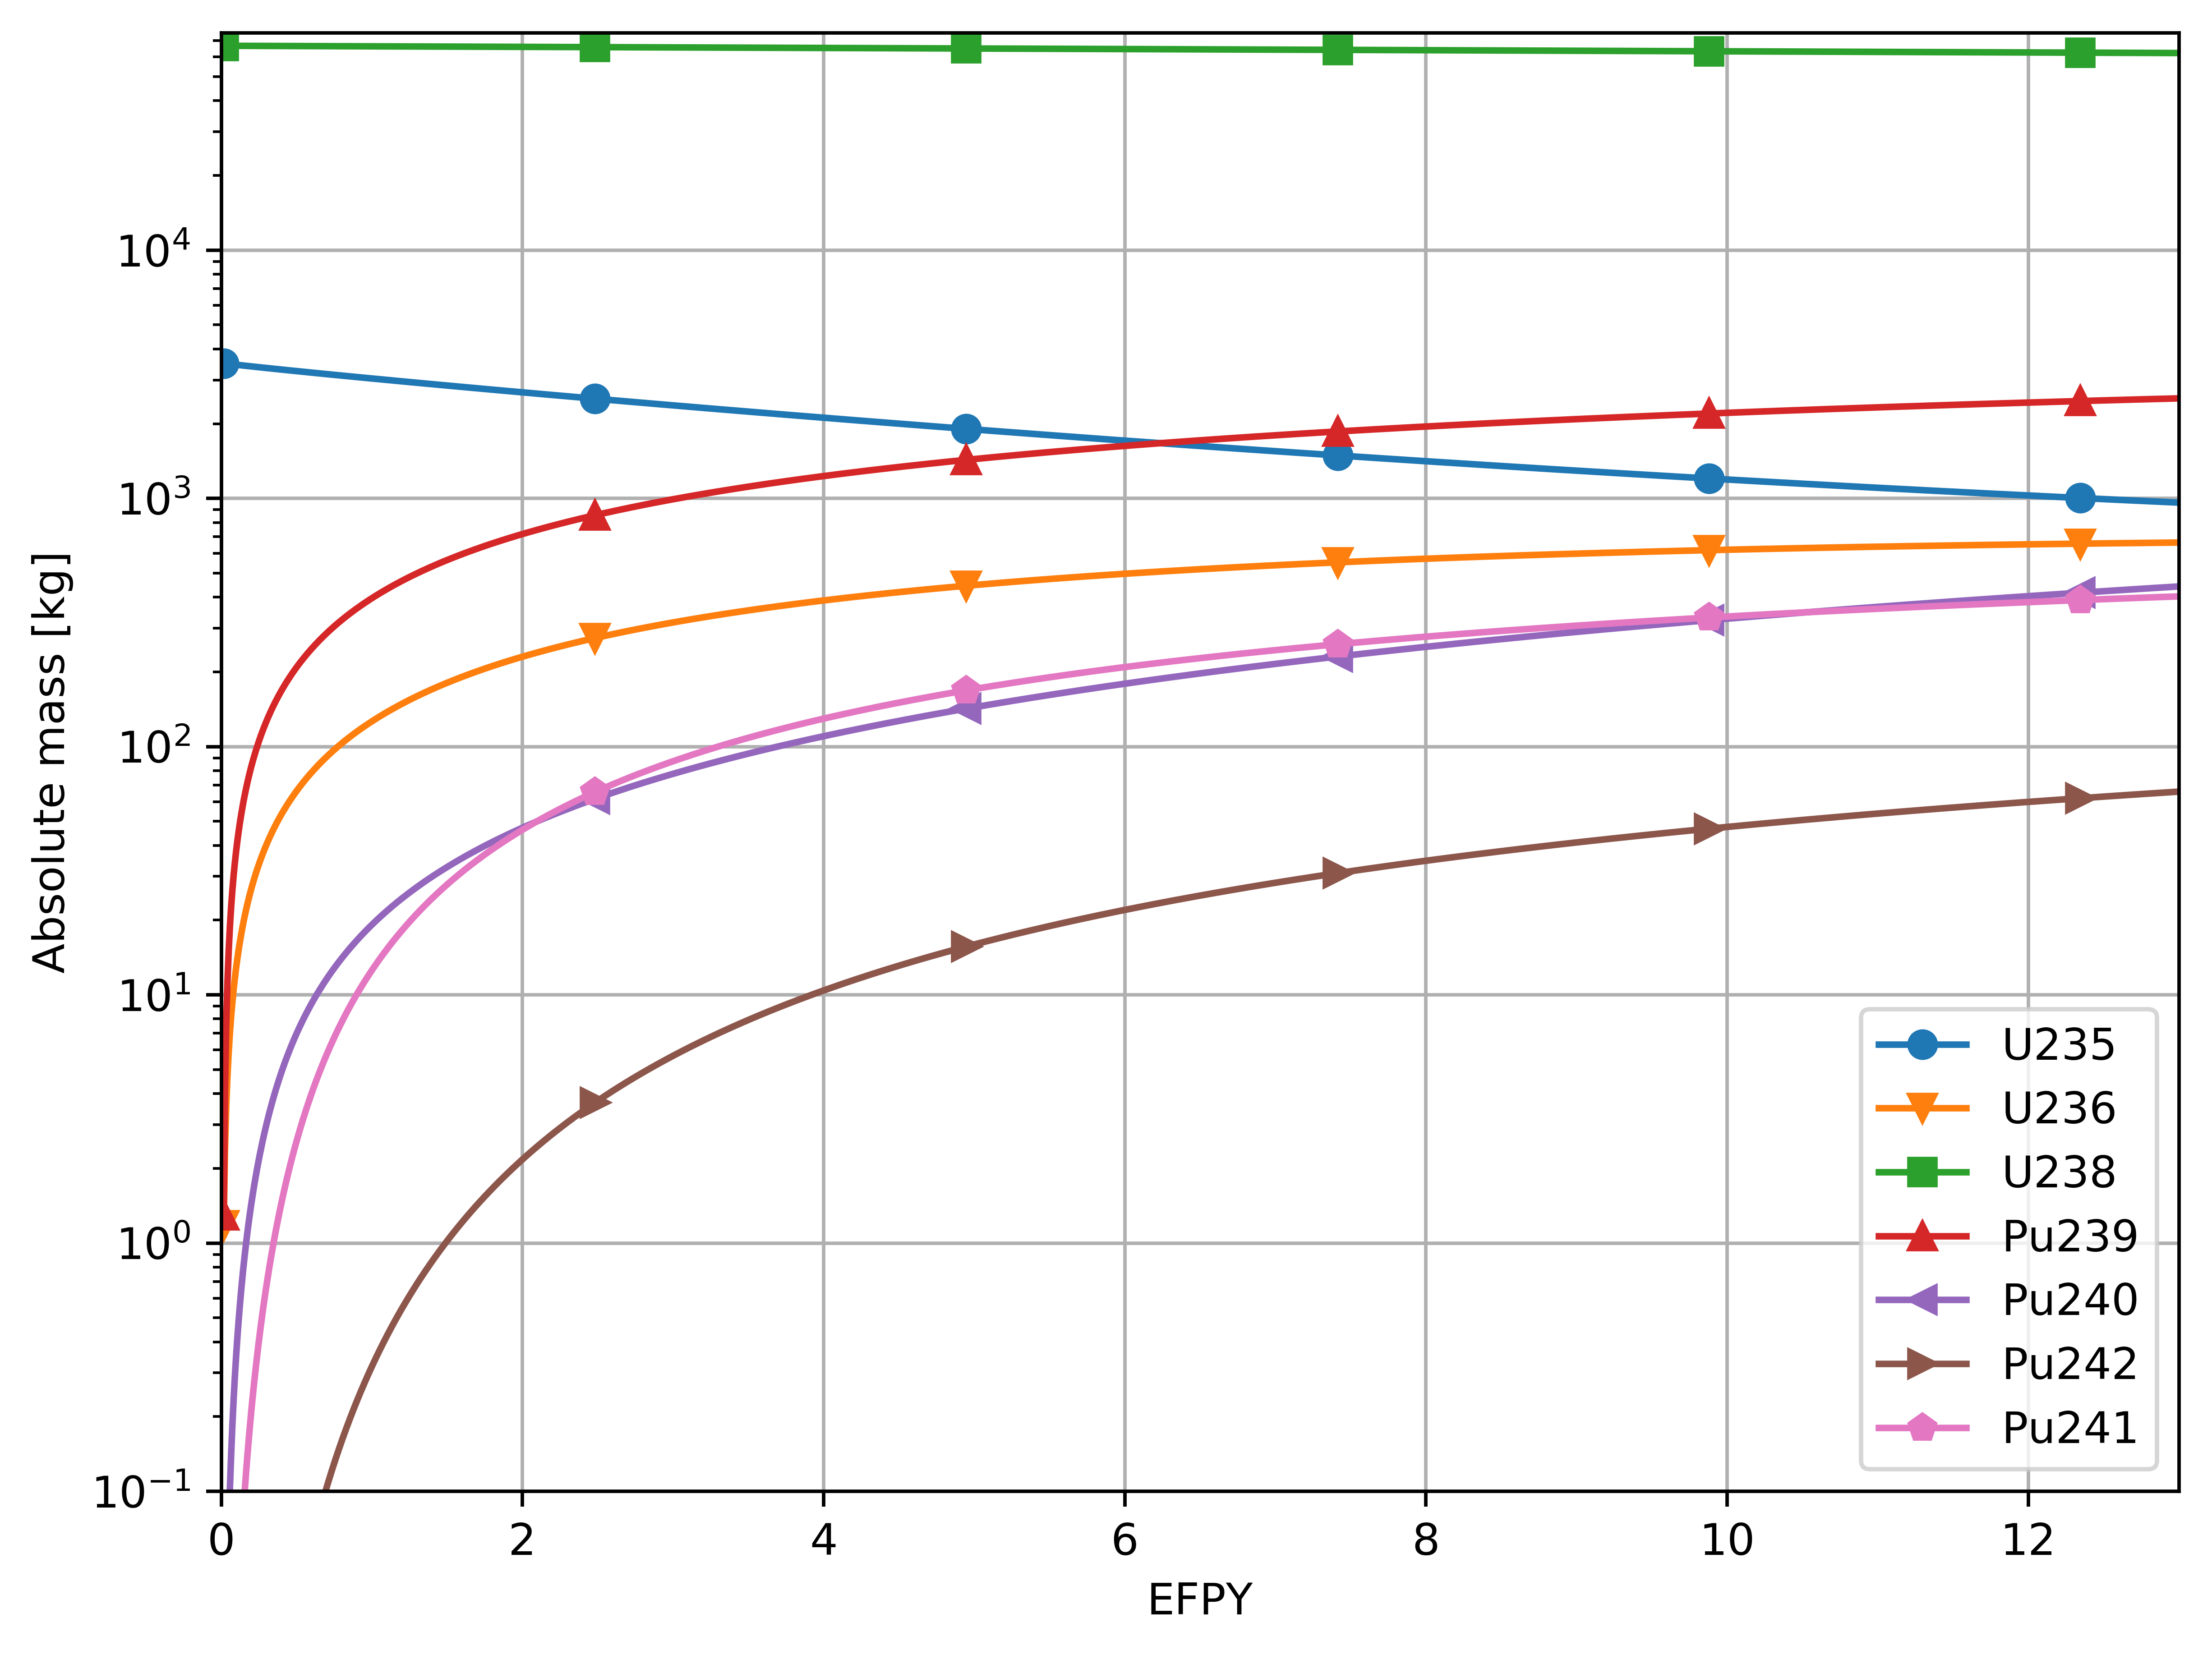
\includegraphics[width=\textwidth]{u_pu_mass.png}
	\caption{Mass of major nuclides during 13 years of reactor operation 
		with 19.79\% \gls{LEU} feed.}
	\label{fig:u-pu}
\end{figure}

I checked correctness of SaltProc v2.0+ by comparing mass of important 
for load-following operation isotopes ($^{135}$Xe, $^{135}$I) to expected 
mass after each depletion step (figure~\ref{fig:xe-i}). For $^{135}$Xe 
expected mass was calculated as follows:
\begin{align}
\qquad\qquad & m_{after\;reprocessing} = m_{before\;reprocessing} \times  
(1-\epsilon_{sparger}) \times (1-\epsilon_{es})
\intertext{where}
m_{after} &= \mbox{mass of the isotope after applying removals and feeds} 
\nonumber \\
m_{before} &= \mbox{mass of the isotope right before  reprocessing} 
\nonumber \\
\epsilon_{sparger} &= \mbox{sparger extraction efficiency} \nonumber \\
\epsilon_{es} &= \mbox{entrainment separator extraction efficiency} 
\nonumber
\end{align}
\begin{figure}[htp!] % replace 't' with 'b' to 
	\centering
	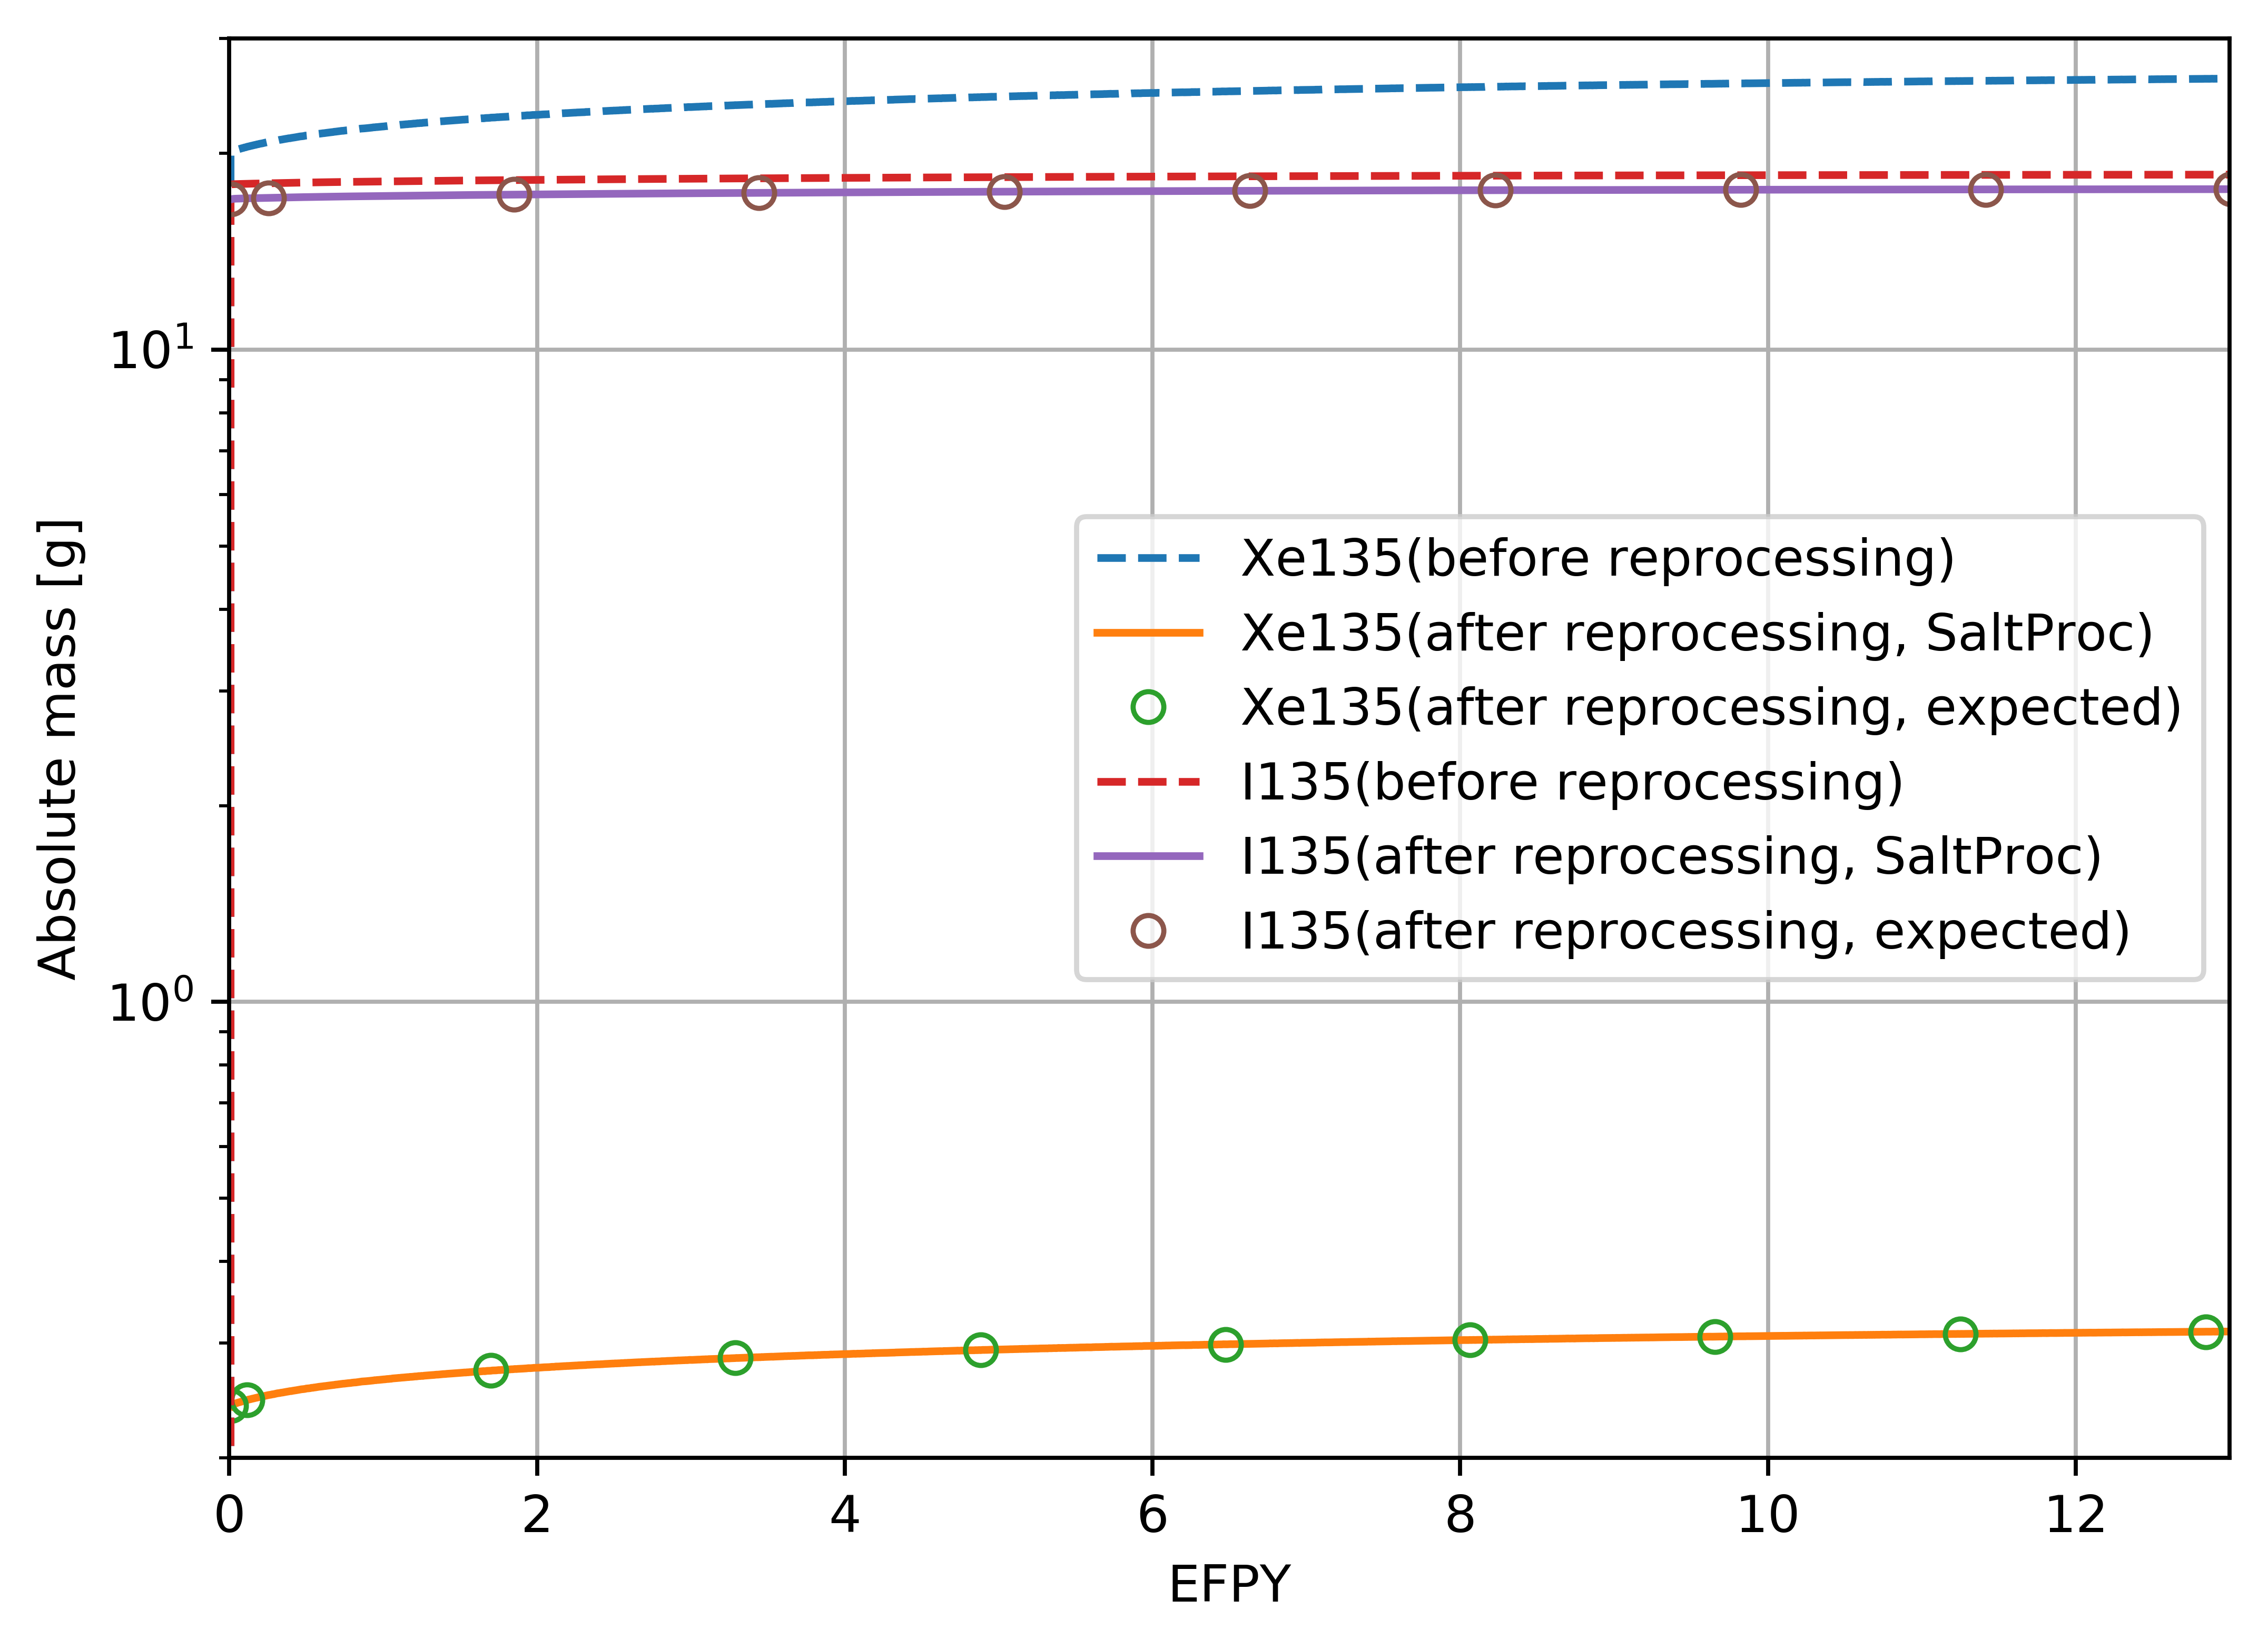
\includegraphics[width=\textwidth]{xe_i_mass.png}
	\caption{Mass of major neutron poison, $^{135}$Xe, and its main precursor, 
		$^{135}$I, during 13 years of reactor operation before and after 
		performing reprocessing in SaltProc v2.0+.}
	\label{fig:xe-i}
\end{figure}

For the iodine approach is similar, but the extraction efficiency of iodine in 
the nickel filter is only 5\%. Figure~\ref{fig:xe-i} shows that SaltProc v2.0+ 
extraction module correctly removes target isotopes with specified extraction 
efficiency: SaltProc and expected mass match. Notably, the \gls{TAP} fuel 
reprocessing system simulated with SaltProc v2.0+ allows keeping $^{135}$Xe 
inventory in the core during operation on 100\% power as low as 1g.
%\chapter[Safety analysis]{Safety analysis}

\section{Safety and operational parameters}

\subsection{Temperature coefficient of reactivity}
The main physical principle underlying the reactor temperature feedback is an 
expansion of heated material. When the fuel salt temperature increases, the 
density of the salt decreases, but at the same time, the total volume of fuel 
salt in the core remains constant because it is bounded by the vessel. When 
the moderator rods temperature increases, the density of zirconium hydride 
decreases, creating additional space for fuel salt. 

Chapter 2, equation~\ref{eq:feedback} defined Total or Isothermal Temperature 
Coefficient (ITC) which expresses the dependence of the core reactivity on the 
combined effects of fuel and moderator temperature. But fuel and moderator 
temperature are rarely equal because fuel heats up much faster than moderator; 
thus, the fuel temperature coefficient (FTC) and the moderator temperature 
coefficient (MTC) should be calculated separately. In the base 
case, the fuel salt and the moderator temperatures are fixed at 900K which is  
operational temperature in the core. To determine the fuel salt temperature 
coefficient (FTC), I will perturbing only the fuel salt temperature to 800K 
and 1000K while fixing the moderator temperature at 900K (base case).  
Likewise, the moderator temperature coefficient (MTC) would be found by 
perturbing the moderator temperature from 900K to 800K and 1000K, while the 
fuel temperature is fixed at 900K. 

The range of temperature perturbation for the TC calculation has been selected 
based on operational parameters. The \gls{TAP} \gls{MSR} operates between 773 
and 973K (500-700$^o$C), which is far below the salt boiling point of 
approximately 1473K. The salt freezes if temperature drops below 773K. At the 
other end of the temperature spectrum, temperature greater than 973K passively 
melt a freeze plug, which drains the fuel salt from the reactor vessel to the  
drain tanks. The drain tanks has subcritical configuration with a high free 
surface area to readily dissipate heat by passive cooling 
\cite{transatomic_power_corporation_technical_2016}. Thus, calculating 
temperature coefficients in temperature range from 800 to 1000K seems to be 
conservative enough to capture outcome most of the accident transients.

Fuel and Moderator Temperature Coefficients for the temperature in range 
from 800 to 900K would be useful for analyzing following transients 
related with sudden fuel salt cooling: 
\begin{itemize}
	\item increase in heat removal by the secondary system;
	\item increase in the fuel salt flow rate;
	\item planned reactor shutdown.
\end{itemize}
Temperature coefficients for the temperature in range from 900 to 1000K 
would be used for transients related with the salt overheat: 
\begin{itemize}
	\item loss-of-coolant accident (LOCA) ;
	\item loss-of-flow accident (LOFA);
	\item loss of ultimate heat sink;
	\item  station blackout (SBO).
\end{itemize}
Thus, temperature coefficients will be calculated separately for heating up 
and cooling. My dissertation will include following  cases: 
\begin{enumerate}
	\item FTC (moderator rods temperature is fixed at 900K):
		\begin{enumerate}[label=(\alph*)]
			\item temperature of the salt rising from 900 to 1000K;
			\item temperature of the salt decreasing from 900 to 800K.
		\end{enumerate}
	\item MTC (the fuel salt temperature is fixed at 900K): 
		\begin{enumerate}[label=(\alph*)]
			\item temperature of the moderator rising from 900 to 1000K;
			\item temperature of the fuel declining from 900 to 800K.
		\end{enumerate}
	\item ITC: 
		\begin{enumerate}[label=(\alph*)]
			\item whole reactor temperature increasing from 900 to 1000K;
			\item whole reactor temperature decreasing from 900 to 800K;
		\end{enumerate}
\end{enumerate}
In the first case, changes in the fuel temperature will impact cross section 
temperature (Doppler broadening) and fuel density but the geometry is 
unchanged because the fuel is a liquid. The density of fuel salt 
changes with respect to temperature as follows \cite{janz_molten_1974}:
\begin{align}\label{eq:salt-den}
\rho_{salt}(T[K]) &= 6.105 - 12.720\times10^4 T \quad [g/cm^3]
\end{align}
In contrast, when the moderator temperature changing, the density, cross 
section temperature, and the geometry are changing also due to thermal 
expansion of the solid zirconium hydride (ZrH$_{1.66}$) rods. Accordingly, the 
new moderator density and sizes will be calculated using a linear temperature 
expansion coefficient of $2.734\times10^{-5}$K$^{-1}$ 
\cite{yamanaka_thermal_1999}. A new geometry input for Serpent 2, which takes 
into account displacement of the moderator  surfaces, will be created based on 
this information. Finally, temperature coefficient for each case will be 
calculated separately as follows:
\begin{align}
\alpha &= \frac{k_{eff}(T_{i+1}) - k_{eff}(T_i)}{k_{eff}(T_{i+1}) 
k_{eff}(T_{i}) (T_{i+1} - T_i)}
\intertext{where}
k_{eff} &= \mbox{effective multiplication factor} \nonumber \\
T_i &= \mbox{fuel salt temperature in (800K, 1000K)} \nonumber
\end{align}
By propagating the $k_{eff}$ statistical error provided by Serpent 2, 
uncertainty for each temperature coefficient will be obtain using formula:
\begin{align}
\delta\alpha &= \abs{\frac{1}{T_{i+1} - T_i}} \sqrt{\frac{\delta 
k_{eff}^2(T_{i+1})}{k_{eff}^4(T_{i+1})}  
+ \frac{\delta k_{eff}^2(T_i)}{k_{eff}^4(T_i)}}
\intertext{where}
\delta k_{eff} &= \mbox{statistical error for $k_{eff}$ from Serpent output} 
\nonumber
\end{align}
Notably, other sources of uncertainty are neglected, such as cross section 
measurement error and approximations inherent in the equations of state 
providing both the salt and moderator density dependence on temperature. 

\subsection{Reactivity control system rod worth}
In the \gls{TAP} concept control rods perform two main functions: to shutdown 
the reactor at any point during operation by introducing sufficient negative 
reactivity, and to control excess of reactivity after moderator rod 
reconfiguration during regular maintenance. In an accident, the control rods 
would be dropped down into the core. The reactivity worth of the control rods  
will be calculated for various positions to separately estimate the worth of 
each control rod, and the whole reactivity control system. Finally, control 
rod with the maximum worth will be localized to conduct basic safety test: at 
\gls{BOL} the reactor should not startup if a single rod (maximum worth rod) 
is accidentally ejected from the \gls{TAP} core.

The reactivity worth of the single control rod is defined as:
\begin{align}
& \qquad\qquad\qquad CRW = (k_{eff}^W - k_{eff}^I)\times 10^5 \;\; [pcm]
\intertext{where}
k_{eff}^W &= \mbox{effective multiplication factor when control rod is fully 
withdrawn} \nonumber \\
k_{eff}^I &= \mbox{effective multiplication factor when control rod is fully 
inserted} \nonumber 
\end{align}
The statistical error of the  reactivity worth will be obtain using formula:
\begin{align}
\delta CRW &= \sqrt{(\delta k_{eff}^W)^2 + (\delta k_{eff}^I)^2}
\intertext{where}
\delta k_{eff}^{W}, \delta k_{eff}^{I}, &= \mbox{$k_{eff}$ statistical error 
from Serpent output} 
\nonumber
\end{align}

\subsection{Axial Offset} \label{sec:axial-offset}
\gls{AOA} refers to a neutron flux depression in the top of a nuclear reactor 
core, which complicates the reactor operation. This problem occurs in  
\gls{PWR} plants and leads to variety of problems: increased local power 
peaking factors, lower that expected burnup and decreased control rod worth.
The Axial Offset is defined as:
\begin{align}
& \qquad\qquad\qquad A/O  = \frac{p_{top} - p_{bottom}}{p_{top} + p_{bottom}}
	\intertext{where}
p_{top}, p_{bottom} &= \mbox{fraction of rated power in a top and bottom half 
of the core} \nonumber
\end{align}

For the case of the \gls{TAP} \gls{MSR}, off-gas system components (e.g., 
sparger, entrainment separator) are introducing small bubbles of an inert gas 
(helium) into the fuel salt during operation. These helium bubbles when enters 
into the core would introduce unpredictable reactivity. Moreover, the diameter 
of the bubbles would raise from the bottom to the top of the core because of 
approximately 140$^{o}$C temperature difference between the reactor inlet and 
outlet. To take into account effect of the gas presence in the fuel salt, I 
will split the reactor core model into few axial regions with different 
corresponding salt density (figure~\ref{fig:axial-offset}).
\begin{figure}[b!] % replace 't' with 'b' to 
	\includegraphics[width=\textwidth]{axial_offset.png}
	\caption{Preliminary schematic view showing the \gls{TAP} model divided to 
	multiple axial layers with different densities of the salt. Assumed linear 
	temperature growth from the bottom to the top.}
	\label{fig:axial-offset}
\end{figure}
The ideal gas law must be employed to find density of the fuel salt with gas 
bubbles\footnote{Assuming we know the bubble number and size from the 
component design.} 
in it:
\begin{align}
PV &= nRT 
\intertext{where}
P &= \mbox{pressure of the gas} \nonumber \\
V &= \mbox{volume of the gas} \nonumber \\
n &= \mbox{number of moles of the gas} \nonumber \\
R &= 8.31 \frac{J}{K\cdot mol} \nonumber \\
T &= \mbox{temperature of the gas} \nonumber
\end{align}
Assuming pressure in the vessel maintained fixed and number of moles of the 
helium is constant, the helium volume change related with temperature change  
can be defined as:
\begin{align}\label{eq:he-vol-change}
&\qquad\qquad\qquad V^{He}_i = \frac{V^{He}_0}{T_0} T_i
\intertext{where}
V^{He}_0, V^{He}_i &= \mbox{total He volume in the salt with temperature 
T$_0$, 
	T$_i$} \nonumber \\
T_0, T_i &= \mbox{temperature of the salt in a lower and i$^{th}$ axial layer} 
\nonumber
\end{align}

Using equations~\ref{eq:salt-den},\ref{eq:he-vol-change}, density of the  
salt/helium mixture in each axial layer ($\rho_i$) will be calculated. 
Finally, Serpent 2 calculation will be performed for the model with 
non-uniform axial density distribution in the fuel salt to determine axial 
neutron flux distribution and axial offset (A/O) in the \gls{TAP} core.

\section{Preliminary results}

\subsection{Temperature coefficients and rod worth at BOL}
Table~\ref{tab:tcoef} summarizes temperature effects on reactivity in the 
\gls{TAP} core calculated for initial fuel salt composition. The fuel 
temperature coefficient is $-0.693$ and $-0.116$ pcm $\Delta k/k\cdot K^{-1}$ 
when perturbing the salt temperature from 900K to 800K and from 900K to 1000K, 
respectively. The MTC and ITC is negative and relatively large for both 
cases. All three temperature coefficients when perturbing from 900K to 
1000K did not matched coefficients when perturbing from 900K to 800K because 
cross sections are nonlinear with respect to temperature.

%%%%%%%%%%%%%%%%%%%%%%%%%%%%%%%%%%%%%%%%
\begin{table}[ht!]
	\caption{Temperature coefficients for the \gls{TAP} reactor at startup for 
	different temperature perturbations.}
	\begin{tabularx}{\textwidth}{ X  r r } \hline
		Reactivity coefficient     & From 900 to 800K [pcm/K] & From 900 to 
		1000K [pcm/K]                  \tabularnewline  \hline
		Fuel salt Temperature Coefficient (FTC) &
		$-0.693\pm9.25\times10^{-2}$ & $-0.116\pm9.33\times10^{-2}$ 
		\tabularnewline \hline
		Moderator (ZrH$_{1.66}$) Temperature Coefficient (MTC) & 
		$-1.106\pm9.25\times10^{-2}$ & $-1.195\pm9.27\times10^{-2}$  
		\tabularnewline \hline
		Isothermal Temperature Coefficient (ITC)  & 
		$-1.768\pm9.17\times10^{-2}$ &  $-1.301\pm9.27\times10^{-2}$  
		\tabularnewline \hline
	\end{tabularx}
	\label{tab:tcoef}
\end{table}
%%%%%%%%%%%%%%%%%%%%%%%%%%%%%%%%%%%%%%%%%%%%%%%%%%%%%%%%%%%%%%%%%%%%%%%%%%%%%%%%
These reactivity coefficients will change most likely during operation due to 
changes in the neutron spectrum, \gls{SVF}, core geometry, amount of fuel in 
the core and fuel composition. The FTC would be expected to be more negative 
during operation as the spectrum thermalizes and additional, non-removing 
fission products and actinides build up in the fuel salt. Temperature 
coefficients should be repeated at middle-of-life and end-of-life to capture 
changes in these characteristics.

A configuration of 25 control rods (Figure~\ref{fig:tap-serpent-plan}) 
provides a reactivity worth of $1110\pm9.7$ pcm (1.1\%) at \gls{BOL}. The 
control rods worth would be expected to become more negative during operation 
because spectrum thermalizes and absorbing material (gadolinium) absorption 
cross section is larger in a thermal energy range. At the same time, that 
effect would be counteracted by the actinides (particularly, plutonium) 
accumulation in the core. Thus, control rod worth change during the reactor 
operation must be estimated.

%\chapter[Future work and Proposed simulations]{Future work and Proposed 
simulations}

\section{Summary}
The need for this work has been shown by a summary of the current state of the 
art of \gls{MSR} depletion simulator capabilities. The literature review in 
Chapter 1 concluded that most \gls{MSR} depletion simulators typically assume 
ideal (rather than realistically constrained) poison removal rates for the 
nuclear system performance modeling. Moreover, most of the simulators assumed 
constant extraction efficiency vectors, which must be determined by the user 
in the input file and cannot be a function of other parameters. The Python 
toolkit, SaltProc v1.0, will directly couple with the Serpent 2 Monte Carlo 
depletion code for liquid-fueled \gls{MSR} depletion simulation to enable 
realistic online reprocessing system modeling. The SaltProc v1.0 seeks to be a 
universal tool for fuel composition evolution analysis in \glspl{MSR} with 
taking into account the complex fuel salt reprocessing system. Such 
reprocessing systems may consist of multiple components with variable removal 
efficiencies and rates. Moreover, these components can be connected in series, 
parallel, or a combination, which will be accurately treated in the SaltProc 
v1.0. Section~\ref{sec:reproc-plant} details the generic design of \gls{MSR}  
fuel salt reprocessing systems. Section~\ref{sec:tool_design} describes the  
SaltProc v1.0 architecture and design that is required to successfully model 
comprehensive liquid-fueled \glspl{MSR} with online fuel reprocessing systems. 

Figure~\ref{fig:workflow} shows an outline of this work. The current chapter 
details each Stage of the proposed work.
 \begin{sidewaysfigure}[ht!] % replace 't' with 'b' to force it to 
 	\centering
 	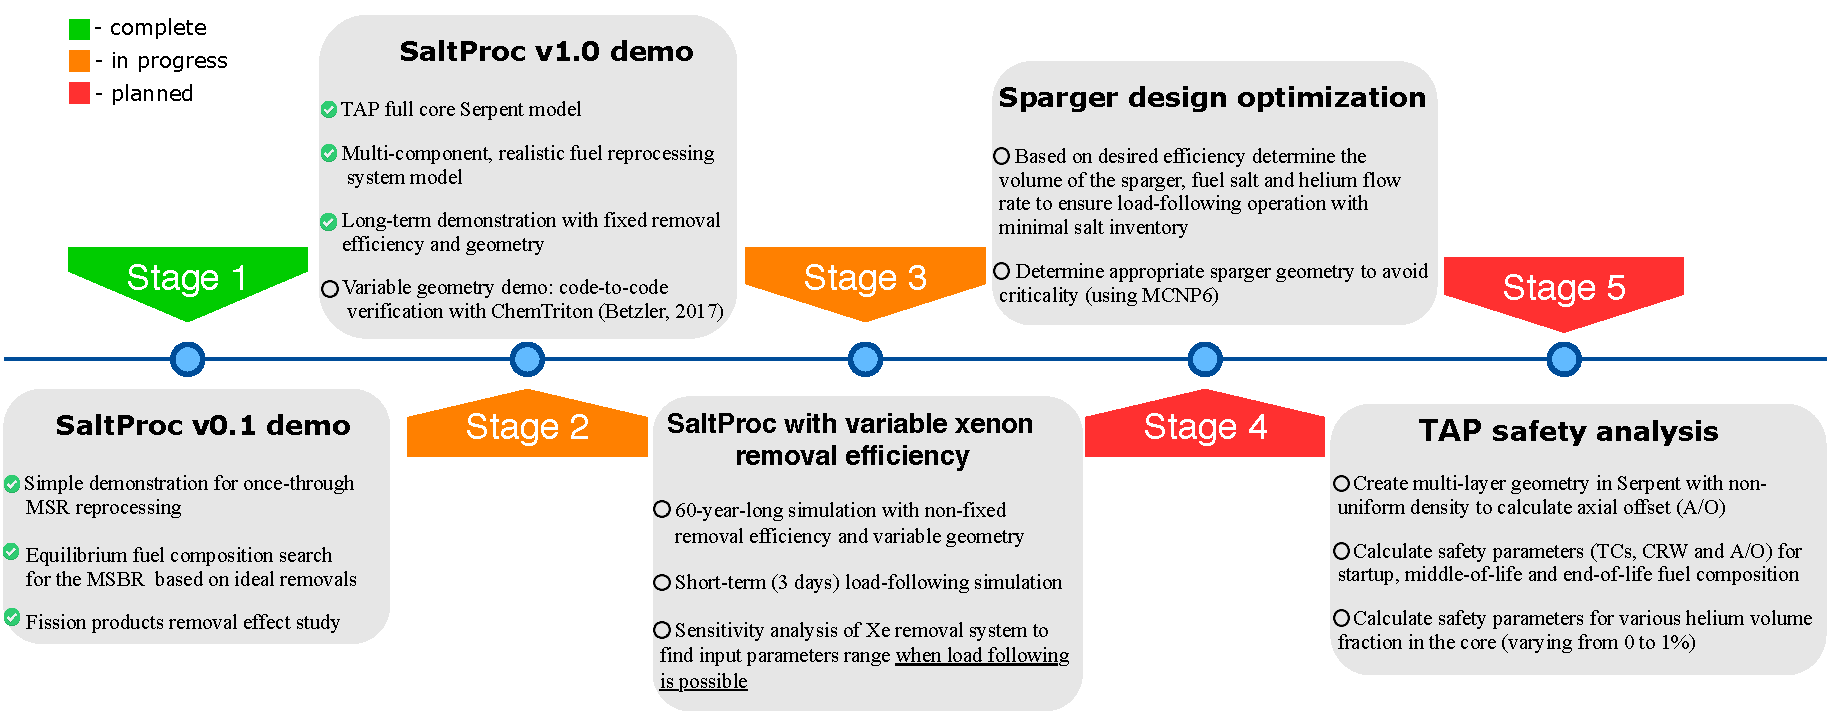
\includegraphics[width=1.06\textwidth]{progress_chart.pdf} 
 	\caption{Workflow for the simulations proposed in this work.}
 	\label{fig:workflow}
 \end{sidewaysfigure}
 \FloatBarrier
 
 
\section{Stage 1: Basic online reprocessing demonstration}
In Stage 1, \gls{MSR} online reprocessing simulation capabilities have been 
reviewed and summarized (Chapter 1). SaltProc v0.1 was demonstrated for 
simplified burnup calculation for the \gls{MSBR} as a part of my M.Sc. thesis  
\cite{rykhlevskii_advanced_2018} and published paper  
\cite{rykhlevskii_modeling_2019}. These efforts illuminated depletion of the 
fuel salt in the \gls{MSBR} for 60 years of operation and took into account 
the following processes:
\begin{enumerate}
	\item \gls{FP} removal from the salt with fixed, ideal extraction 
	efficiencies (the fuel reprocessing system removed 100\% of target 
	poisons).
	\item $^{233}$Pa removal (100\%) and feed of an equal mass of $^{233}$U 
	into the core (instantaneous $^{233}$Pa decay to $^{233}$U was assumed).
	\item Fresh fertile material ($^{232}$Th) feed to maintain the constant 
	fuel salt inventory.
\end{enumerate}
Additionally, the effect of removing fission products from the fuel salt was 
investigated separately for a different group of \glspl{FP} (noble gases, 
noble and seminoble metals, rare earth elements). As expected, removing  
fission products provides significant neutronic benefit and enables a longer 
core lifetime. Section~\ref{sec:pre-results-msbr} described key findings after 
completing Stage 1.

\section{Stage 2: SaltProc v1.0 demonstration and validation for the TAP}
Simulating a realistic multi-component fuel reprocessing system is important 
for calculating an accurate fuel salt composition. SaltProc v0.1 was 
completely refactored for modeling a complicated salt reprocessing system. To 
demonstrate SaltProc v1.0 capabilities, we have created a full-core \gls{TAP} 
\gls{MSR} model in Serpent 2 \cite{chaube_tap_2019} which was described in 
detail in Section~\ref{sec:tap_model}. Moreover, the multi-component fuel 
reprocessing system of the \gls{TAP} was developed on this stage 
(Section~\ref{sec:stage2-demo}). Section~\ref{sec:stage2-demo} also presented 
preliminary results of Stage 2. The Stage 2 demonstration case has following 
advantages over Stage 1:
\begin{itemize}
	\item SaltProc v0.1 (Stage 1) approximated the fuel salt reprocessing 
	system 
	as a single ``black'' box, which removes the entire mass (100\% removal 
	efficiency) of processed elements at once. In contrast, SaltProc v1.0 
	treats the fuel reprocessing system as a complex structure of components, 
	each removing a specific set of elements with specific extraction 
	efficiency. 
	\item SaltProc v1.0 inherently checks mass conservation at each depletion 
	step and dynamically calculates feed stream to maintain the fuel salt 
	inventory constant.
	\item SaltProc v1.0 tracks the waste stream from each component.
\end{itemize}

The foremost future effort in this stage is to enable switching between 
multiple Serpent geometries during simulation. For the \gls{TAP} concept, the 
number of moderator rods in the core varies from 1332 at the startup to 6700 
at the \gls{EOL}. The user will have an option to choose when SaltProc v1.0 
should switch to next geometry: (1) after a specific depletion  time (e.g., 18 
months which is a common maintenance/refueling shutdown interval for 
\glspl{LWR}); or (2) when the effective multiplication factor reaches a 
specific value (e.g., $1.00<k_{eff} < 1.002$). Additionally, SaltProc v1.0 
will correct the total fuel salt inventory in the primary loop to compensate 
for the core geometry change. Overall, the adjustable geometry capability will 
realistically simulate long-term (60 year) operation of the \gls{TAP} reactor 
to obtain accurate fuel salt composition at different moments during operation.

Results obtained in Stage 2 will be used for code-to-code verification with  
ChemTriton/Shift results for full-core \gls{TAP} core geometry from the most 
recent \gls{ORNL} technical report TM-2017/475 \cite{betzler_assessment_2017}. 
Notably, the fuel salt composition evolution during the \gls{TAP} reactor 
operation and corresponding core geometry are determinative for all next 
stages.

This work is developed with a test-driven development paradigm. Specifically, 
before any new functionality is implemented, a suite of tests is written, 
which as carefully define its expected behavior as possible. The code is then 
written to pass the test suite. In this way, the tool developed in this work 
is expected to be comprehensively tested in parallel with its development. 
Thus, after code-to-code verification with ChemTriton/Shift multiple-component 
integration tests will be added to the test harness to make sure that future 
changes in the code will not break previous functionality.

Test problems will help comprehensively define and confirm each unit of the 
demonstration functionality. These problems will include fundamental, 
information-passing tests as well as more challenging multiple-component 
integration tests. Every unit of functionality within the toolkit will be 
tested as an integral part of development.

This milestone will result in a processing system model capable of simulating
various liquid-fueled \glspl{MSR} with multi-component fuel reprocessing 
systems but with constant separation efficiencies, defined at runtime. 
Additionally, this stage will demonstrate a key feature of the \gls{TAP} 
\gls{MSR} - adjusting the moderator rod configuration - which is necessary to 
maintain the reactor criticality during the 60-years lifetime. 

\section{Stage 3: Variable xenon extraction rate}
When Stage 2 is complete, a series of extensions to the Stage 2 model will 
be pursued. These will incorporate extraction efficiencies as a function of 
many physical system design parameters (e.g., void fraction in the salt, 
helium bubble size). Mathematical correlations for the efficiencies will be 
taken from relationships in the literature \cite{peebles_removal_1968, 
gabbard_development_1974} and CFD simulations currently being conducted 
at the University of Illinois at Urbana-Champaign \cite{huff_enabling_2018}. 
For demonstration proposes, just xenon removal efficiency will be defined as a 
function of many parameters (Section~\ref{sec:gas-separ}) due to 
limited data provided in the listed literature. For other fission products  
from the \gls{TAP} reprocessing scheme (table~\ref{tab:reprocessing_list}), 
removal efficiencies will be defined based on the removal rates from the 
table, assuming time-independent extraction efficiency. This milestone will 
result in a realistic online reprocessing system model capable of modeling 
\gls{MSR} systems with parameterized, realistically achievable process rates,  
and extraction efficiencies.

Another anticipated extension will test the \gls{TAP} reactor ability to 
operate in a load-following regime. Short-term (3 days) depletion using 
SaltProc v1.0 will be performed with the core power changing in the [0, 100\%] 
range with a ramp rate 10\%/min (to be competitive with natural gas peaking 
plants, which ramp at or above 10\% of their capacity) 
\cite{huff_enabling_2018}. 
Figure~\ref{fig:load} shows the load curve selected to demonstrate the 
worst-case scenario of load-following:
\begin{enumerate}
	\item Startup with fresh fuel and operating on 100\% of \gls{HFP}
level 
	for 40 hours to reach $^{135}$Xe/$^{135}$I equilibrium;
	\item Load-following power drop (0.1 \gls{HFP}/min), from \gls{HFP} 
	to \gls{HZP};
	\item Shutdown for 8 hours\footnote{At startup. Time after shutdown when 
	$^{135}$Xe concentration would reach maximum value greatly depends on 
	neutron energy spectrum which for the \gls{TAP} concept changes 
	significantly during operation.} to reach the $^{135}$Xe peak;
	\item Load-following power rise (0.1 \gls{HFP}/min), from \gls{HZP} 
	to \gls{HFP}.
\end{enumerate}
This scenario can be considered as backing up solar power with
nuclear on a 
high-solar penetration grid (e.g., in California).
\begin{figure}[bth!] % replace 't' with 'b' to 
	\centering
	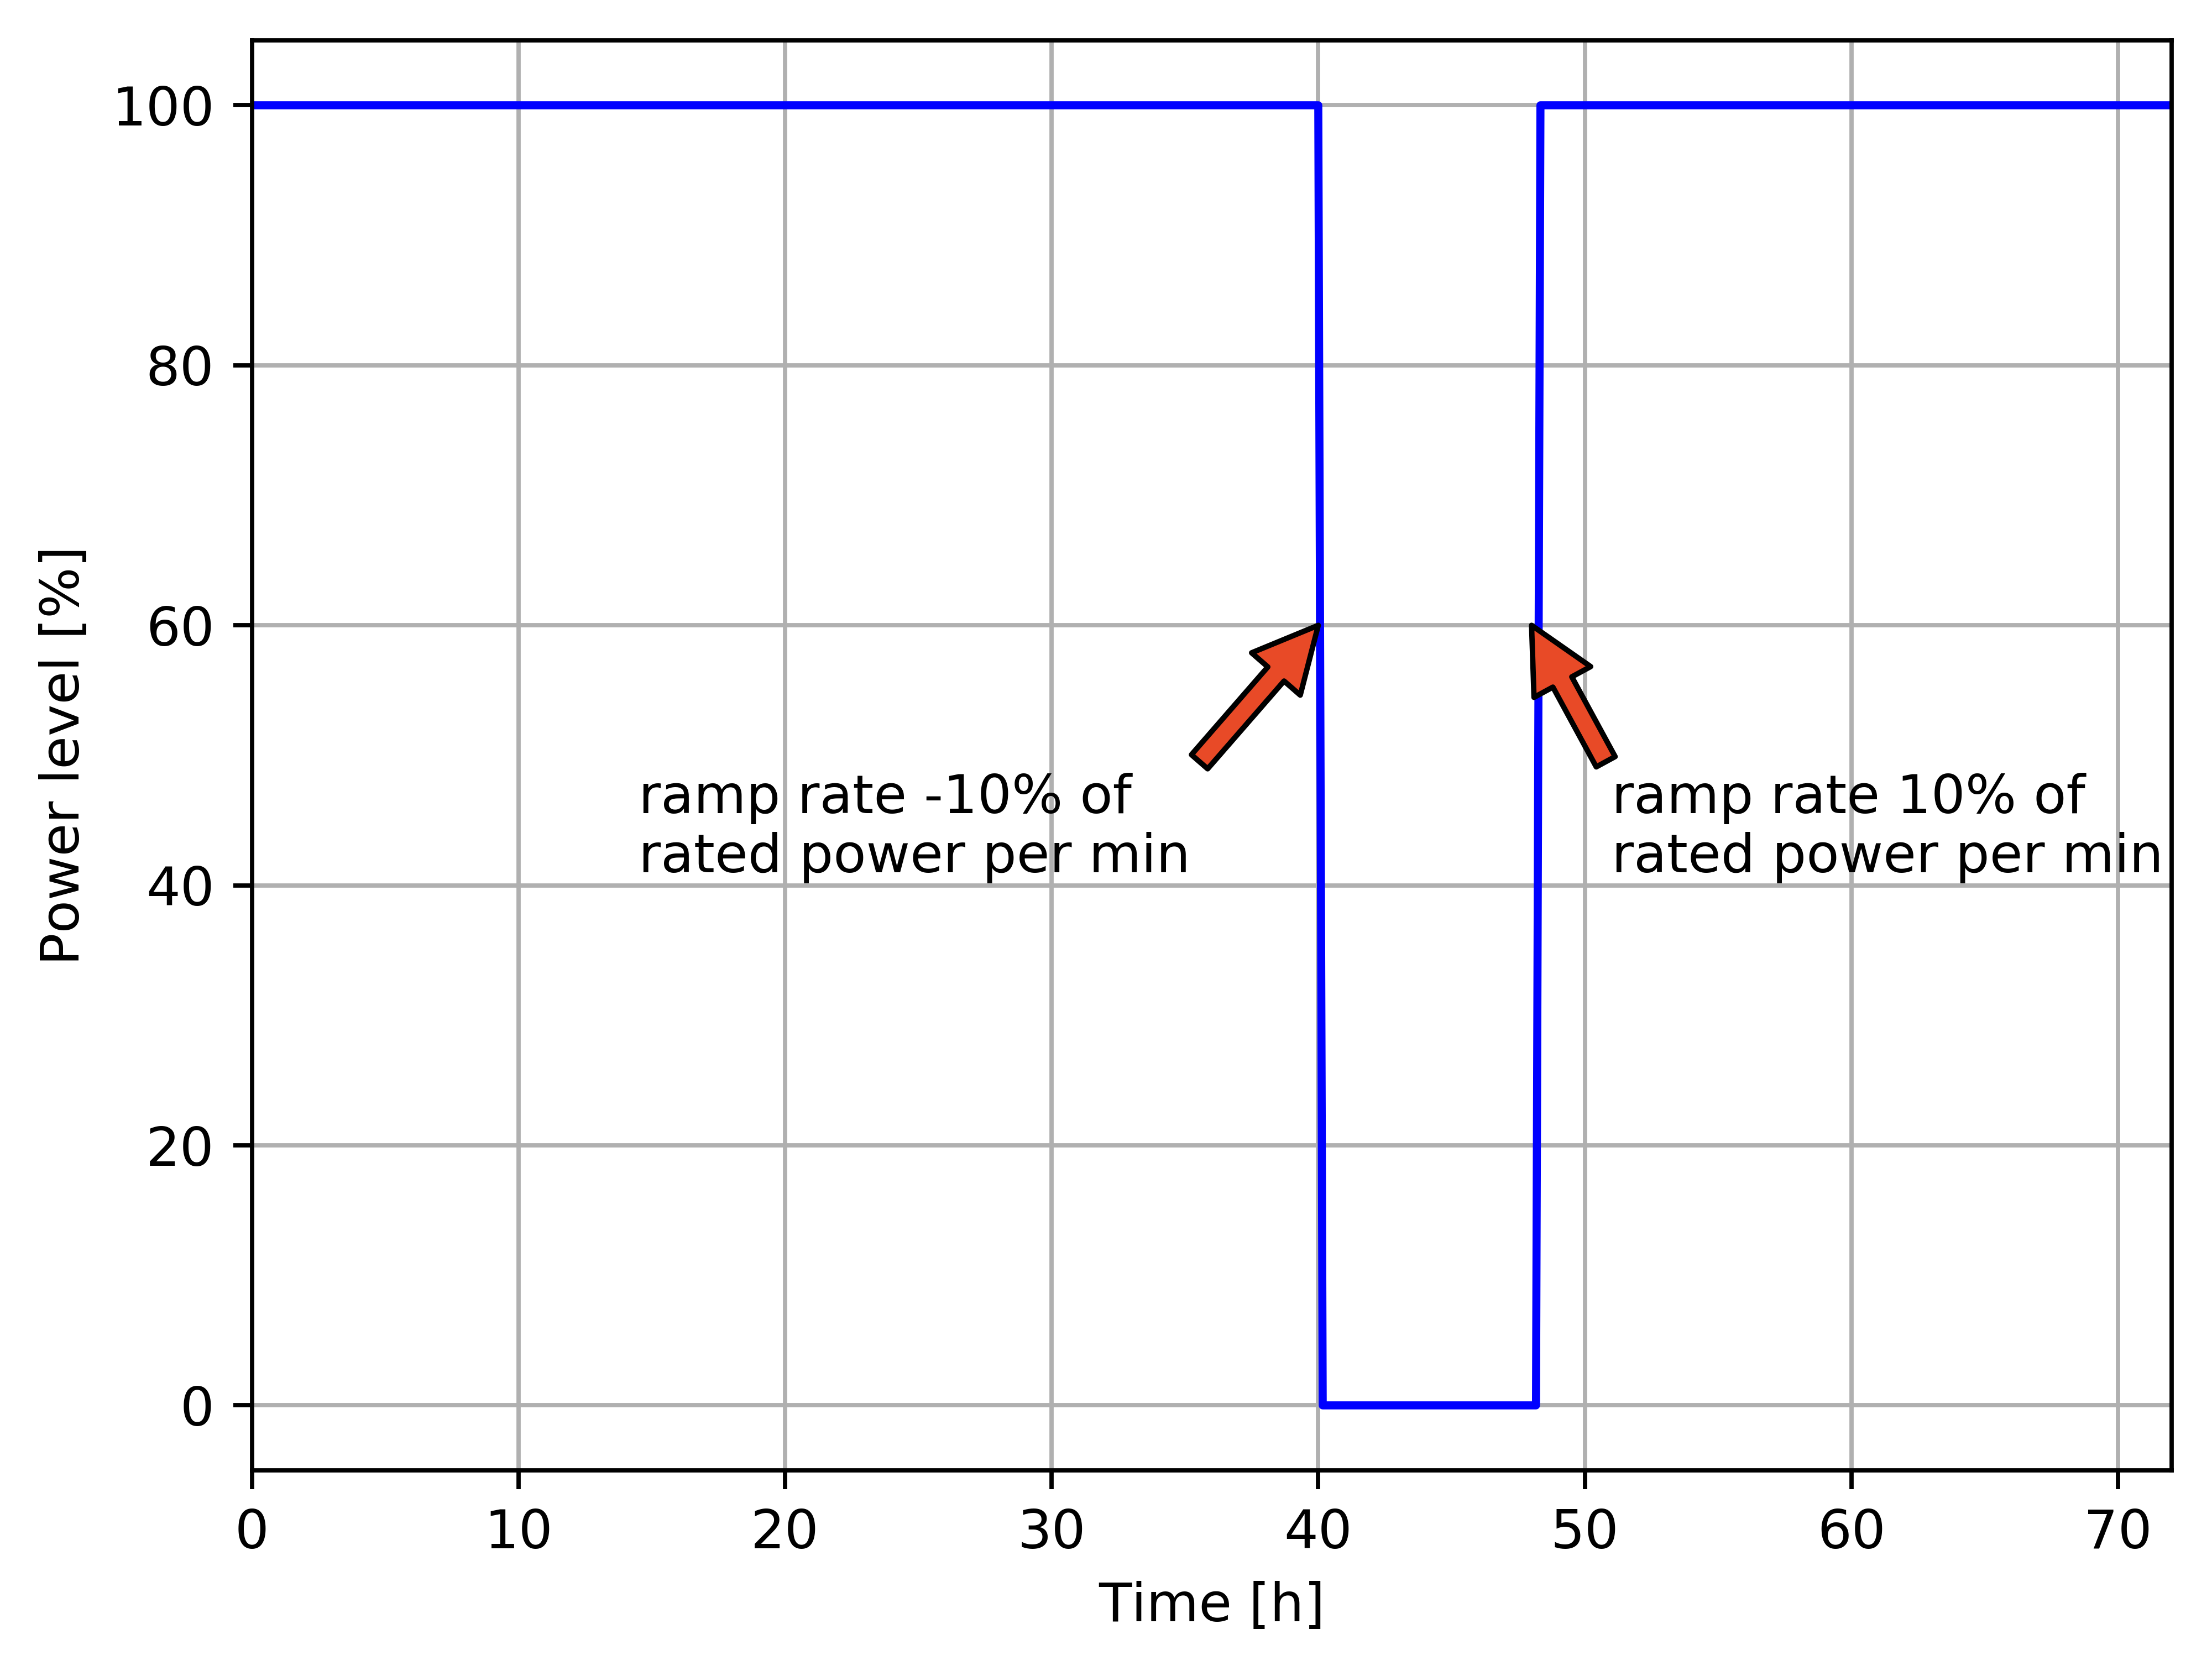
\includegraphics[width=0.8\textwidth]{load_curve.png}
	\caption{Tentative load curve for short-term load-following depletion 
	simulation for the \gls{TAP} reactor using SaltProc v1.0.}
	\label{fig:load}
\end{figure}

The depletion step time for short-term simulation will be varied in a range 
from 1 to 60 min to find a compromise between accuracy and computational cost. 
It is expected that load-following performance will be better at the \gls{BOL} 
because the neutron energy spectrum thermalizes during the reactor operation. 
Thus, the short-term load-following simulation will be repeated for the 
\gls{BOL}, the middle of life, and the \gls{EOL} to assess the \gls{TAP} 
concept performance in a load-following regime during the whole reactor 
lifetime.

Additionally, sensitivity analysis of input parameters in the xenon extraction 
correlation will be conducted to determine the range of key parameters (e.g., 
mass transfer coefficient, helium sparging rate, gas-liquid interfacial area, 
temperature) when load-following is possible for the \gls{TAP} reactor in a 
worst-case power demand scenario. These multiple system configurations  
incorporating user-parametrized components in the fuel salt processing system 
will be collected and published in a \textit{.json}-compatible database for 
use with the SaltProc v1.0 to encourage further research in this area.

\section{Stage 4: Prototype design for the Xe removal system}
As the model becomes capable of incorporating user-parametrized components 
with correlation-based extraction efficiency for the helium sparging 
component, constraints bounding a suitable sparger design will be determined 
and described. These design ranges (i.e., helium sparging rate) obtained from 
the previous Stage. The ultimate objective of the design is to ensure 
load-following operation during most of the operation period when 
minimizing the fuel salt inventory. That is, constrained optimization problem 
must be solved to minimize total fuel salt volume outside of the core. The 
target design parameters for the sparger include: the volume of sparger, 
helium flow rate, salt flow rate, and geometry.

Additionally, nuclear criticality safety analysis will be performed using 
MCNP6 \cite{werner_mcnp6._2018} to confirm that the selected sparger design 
has a subcritical configuration. If the sparger geometry obtained during the 
optimization process is supercritical, the fission gas removal system would 
contain multiple spargers of smaller size connected in parallel. Total fuel 
salt volume and sparger size are expected to be smaller at the \gls{BOL} and 
increase steadily as the neutron energy spectrum becomes softer.

\section{Stage 5: \gls{TAP} Safety Analysis}
The objective of this Stage is to characterize neutronics limits related to 
load following. High-fidelity simulations will achieve this goal with the 
Serpent 2 Monte Carlo code. Specifically, changes in safety parameters 
(Section~\ref{sec:safety-param}) will be evaluated for two time frames:
\begin{enumerate}
	\item Long-time-scale changes in safety parameters should not compromise 
	\gls{TAP} \gls{MSR} safety.
	\item Load-following operation at key moments in the reactor lifetime 
	(e.g., at startup, at the middle of life, at the end of life) must not 
	result in significant changes in safety parameters.
\end{enumerate}
Section~\ref{sec:safety-param-res} showed preliminary calculations of  
temperature coefficients and reactivity control system worth for the \gls{TAP} 
at startup. The next step will develop a axially discretized core geometry in 
Serpent with non-uniform axial density distribution to estimate the axial 
power offset. Afterward, safety parameters will be calculated at the 
\gls{BOL}, the middle of life, and the \gls{EOL} to capture safety parameter  
variation over long time scales. Validation against previous work in a 
collaboration between Transatomic Power and ORNL 
\cite{betzler_assessment_2017, betzler_fuel_2018} will also be 
performed for confidence building. Additionally, analysis for different xenon 
removal efficiencies (i.e., in the range from 0 to 100\%) will be performed to 
capture the effect of $^{135}$Xe concentration on safety.

To analyze the impact of the load-following operation on \gls{TAP} concept 
safety, safety parameter calculations will be repeated for the load-following 
transient. The combination of fuel and moderator temperature coefficients must 
remain strongly negative, and the reactivity worth of control rods must be 
sufficient to shut down the reactor for all times during load-following 
operation. 

\section{Conclusions}
Details of gas removal and fuel salt processing systems in liquid-fueled 
\glspl{MSR} have historically been conceptual rather than concrete. Usually, 
researchers assume ideal rather than realistically constrained poison 
extraction efficiency for reactor performance calculations. This work will 
more realistically model an online molten salt processing system with a focus 
on the gas removal system of the prospective \gls{TAP} \gls{MSR}. SaltProc, a 
Python toolkit was developed as a part of this work. SaltProc couple directly 
with the Serpent 2 Monte Carlo burnup software to capture the evolution of 
fuel salt composition during reactor operation in the context of an online 
fuel processing system.

Modeling and simulation of the online reprocessing system in the \gls{MSR} 
has shown promise in past research. Our work on simulating online fuel  
reprocessing for the thorium-fueled \gls{MSBR} yielded interesting results: 
notable neutron energy spectrum shift and corresponding changes in safety 
parameters during operation. Additional preliminary work also showed promise 
results in modeling a simplified fuel processing system for the \gls{TAP} 
\gls{MSR}. These simulations motivate future work in modeling advanced 
liquid-fueled \gls{MSR} plant designs.

To establish a feasible system design for molten salt fuel reprocessing, a 
more advanced model of the \gls{TAP} \gls{MSR} system with adjustable core 
geometry and realistically achievable extraction efficiencies will be 
developed. Extended SaltProc v1.0 will realistically capture the dynamics of 
fuels salt composition changes with higher accuracy. SaltProc v1.0 will also 
be employed to simulate the \gls{TAP} \gls{MSR} behavior in short-term 
transients to determine the feasibility of load following. Additionally, input 
parameters such as flow rates, bubble size, and the void fraction will be 
varied to determine the range of these parameters when the load following is 
possible for the \gls{TAP} concept.

In addition to these simulations, several extensions are suggested to 
advance our preliminary work. First, the feasible design parameters of the 
sparger, critical component of the \gls{TAP} gas removal system, will be 
optimized through sensitivity analysis of geometry and system conditions. To 
guarantee criticality safety,an MCNP6 simulation will be performed to define 
an appropriate sparger geometry. Further effort will focus on safety  
parameter evolution in the \gls{TAP} reactor during lifetime (60 years),  
when the moderator rod configuration discretely changes. Finally, dynamics of 
the safety parameters will be investigated for a short-term case: load 
following for three days with fixed moderator configuration and worst-case 
scenario of the power level change. 



%%%%%%%%%%%%%%%%%%%%%%%%%%%%%%%%%%%%%%%%%%%%%%%%%%%%%%%%%%%%%%%%%%%%%%%%%%%%%%%
% APPENDIX
%
%\appendix
%\include{apx}

\backmatter

%%%%%%%%%%%%%%%%%%%%%%%%%%%%%%%%%%%%%%%%%%%%%%%%%%%%%%%%%%%%%%%%%%%%%%%%%%%%%%%
% BIBLIOGRAPHY
%
%\bibliographystyle{IEEE_ECE}
\bibliographystyle{unsrt}
% Put references in BibTeX format in thesisrefs.bib.
\bibliography{thesisrefs}

\end{document}
\endinput
